\documentclass[twoside]{book}

% Packages required by doxygen
\usepackage{fixltx2e}
\usepackage{calc}
\usepackage{doxygen}
\usepackage[export]{adjustbox} % also loads graphicx
\usepackage{graphicx}
\usepackage[utf8]{inputenc}
\usepackage{makeidx}
\usepackage{multicol}
\usepackage{multirow}
\PassOptionsToPackage{warn}{textcomp}
\usepackage{textcomp}
\usepackage[nointegrals]{wasysym}
\usepackage[table]{xcolor}

% Font selection
\usepackage[T1]{fontenc}
\usepackage[scaled=.90]{helvet}
\usepackage{courier}
\usepackage{amssymb}
\usepackage{sectsty}
\renewcommand{\familydefault}{\sfdefault}
\allsectionsfont{%
  \fontseries{bc}\selectfont%
  \color{darkgray}%
}
\renewcommand{\DoxyLabelFont}{%
  \fontseries{bc}\selectfont%
  \color{darkgray}%
}
\newcommand{\+}{\discretionary{\mbox{\scriptsize$\hookleftarrow$}}{}{}}

% Page & text layout
\usepackage{geometry}
\geometry{%
  a4paper,%
  top=2.5cm,%
  bottom=2.5cm,%
  left=2.5cm,%
  right=2.5cm%
}
\tolerance=750
\hfuzz=15pt
\hbadness=750
\setlength{\emergencystretch}{15pt}
\setlength{\parindent}{0cm}
\setlength{\parskip}{0.2cm}
\makeatletter
\renewcommand{\paragraph}{%
  \@startsection{paragraph}{4}{0ex}{-1.0ex}{1.0ex}{%
    \normalfont\normalsize\bfseries\SS@parafont%
  }%
}
\renewcommand{\subparagraph}{%
  \@startsection{subparagraph}{5}{0ex}{-1.0ex}{1.0ex}{%
    \normalfont\normalsize\bfseries\SS@subparafont%
  }%
}
\makeatother

% Headers & footers
\usepackage{fancyhdr}
\pagestyle{fancyplain}
\fancyhead[LE]{\fancyplain{}{\bfseries\thepage}}
\fancyhead[CE]{\fancyplain{}{}}
\fancyhead[RE]{\fancyplain{}{\bfseries\leftmark}}
\fancyhead[LO]{\fancyplain{}{\bfseries\rightmark}}
\fancyhead[CO]{\fancyplain{}{}}
\fancyhead[RO]{\fancyplain{}{\bfseries\thepage}}
\fancyfoot[LE]{\fancyplain{}{}}
\fancyfoot[CE]{\fancyplain{}{}}
\fancyfoot[RE]{\fancyplain{}{\bfseries\scriptsize Generated on Fri Apr 1 2016 06\+:41\+:44 for Introduction\+\_\+to\+\_\+\+Algorithms by Doxygen }}
\fancyfoot[LO]{\fancyplain{}{\bfseries\scriptsize Generated on Fri Apr 1 2016 06\+:41\+:44 for Introduction\+\_\+to\+\_\+\+Algorithms by Doxygen }}
\fancyfoot[CO]{\fancyplain{}{}}
\fancyfoot[RO]{\fancyplain{}{}}
\renewcommand{\footrulewidth}{0.4pt}
\renewcommand{\chaptermark}[1]{%
  \markboth{#1}{}%
}
\renewcommand{\sectionmark}[1]{%
  \markright{\thesection\ #1}%
}

% Indices & bibliography
\usepackage{natbib}
\usepackage[titles]{tocloft}
\setcounter{tocdepth}{3}
\setcounter{secnumdepth}{5}
\makeindex

% Hyperlinks (required, but should be loaded last)
\usepackage{ifpdf}
\ifpdf
  \usepackage[pdftex,pagebackref=true]{hyperref}
\else
  \usepackage[ps2pdf,pagebackref=true]{hyperref}
\fi
\hypersetup{%
  colorlinks=true,%
  linkcolor=blue,%
  citecolor=blue,%
  unicode%
}

% Custom commands
\newcommand{\clearemptydoublepage}{%
  \newpage{\pagestyle{empty}\cleardoublepage}%
}


%===== C O N T E N T S =====

\begin{document}

% Titlepage & ToC
\hypersetup{pageanchor=false,
             bookmarks=true,
             bookmarksnumbered=true,
             pdfencoding=unicode
            }
\pagenumbering{roman}
\begin{titlepage}
\vspace*{7cm}
\begin{center}%
{\Large Introduction\+\_\+to\+\_\+\+Algorithms }\\
\vspace*{1cm}
{\large Generated by Doxygen 1.8.10}\\
\vspace*{0.5cm}
{\small Fri Apr 1 2016 06:41:44}\\
\end{center}
\end{titlepage}
\clearemptydoublepage
\tableofcontents
\clearemptydoublepage
\pagenumbering{arabic}
\hypersetup{pageanchor=true}

%--- Begin generated contents ---
\chapter{Namespace Index}
\section{Namespace List}
Here is a list of all namespaces with brief descriptions\+:\begin{DoxyCompactList}
\item\contentsline{section}{\hyperlink{namespace_introdunction_to_algorithm}{Introdunction\+To\+Algorithm} \\*Namespace of \hyperlink{namespace_introdunction_to_algorithm}{Introdunction\+To\+Algorithm} }{\pageref{namespace_introdunction_to_algorithm}}{}
\item\contentsline{section}{\hyperlink{namespace_introdunction_to_algorithm_1_1_select_algorithm}{Introdunction\+To\+Algorithm\+::\+Select\+Algorithm} \\*Namespace of \hyperlink{namespace_introdunction_to_algorithm_1_1_select_algorithm}{Select\+Algorithm} }{\pageref{namespace_introdunction_to_algorithm_1_1_select_algorithm}}{}
\item\contentsline{section}{\hyperlink{namespace_introdunction_to_algorithm_1_1_sort_algorithm}{Introdunction\+To\+Algorithm\+::\+Sort\+Algorithm} \\*Namespace of \hyperlink{namespace_introdunction_to_algorithm_1_1_sort_algorithm}{Sort\+Algorithm} }{\pageref{namespace_introdunction_to_algorithm_1_1_sort_algorithm}}{}
\end{DoxyCompactList}

\chapter{Hierarchical Index}
\section{Class Hierarchy}
This inheritance list is sorted roughly, but not completely, alphabetically\+:\begin{DoxyCompactList}
\item \contentsline{section}{Introdunction\+To\+Algorithm\+:\+:Tree\+Algorithm\+:\+:Binary\+Tree$<$ Node\+Type $>$}{\pageref{struct_introdunction_to_algorithm_1_1_tree_algorithm_1_1_binary_tree}}{}
\begin{DoxyCompactList}
\item \contentsline{section}{Introdunction\+To\+Algorithm\+:\+:Tree\+Algorithm\+:\+:Search\+Tree$<$ Node\+Type $>$}{\pageref{class_introdunction_to_algorithm_1_1_tree_algorithm_1_1_search_tree}}{}
\end{DoxyCompactList}
\item \contentsline{section}{Introdunction\+To\+Algorithm\+:\+:Tree\+Algorithm\+:\+:Binary\+Tree$<$ Node $>$}{\pageref{struct_introdunction_to_algorithm_1_1_tree_algorithm_1_1_binary_tree}}{}
\begin{DoxyCompactList}
\item \contentsline{section}{Introdunction\+To\+Algorithm\+:\+:Tree\+Algorithm\+:\+:Search\+Tree$<$ Node $>$}{\pageref{class_introdunction_to_algorithm_1_1_tree_algorithm_1_1_search_tree}}{}
\end{DoxyCompactList}
\item \contentsline{section}{Introdunction\+To\+Algorithm\+:\+:Tree\+Algorithm\+:\+:Binary\+Tree\+Node$<$ T $>$}{\pageref{struct_introdunction_to_algorithm_1_1_tree_algorithm_1_1_binary_tree_node}}{}
\item \contentsline{section}{Introdunction\+To\+Algorithm\+:\+:Sort\+Algorithm\+:\+:Sort\+\_\+\+Heap$<$ Iterator, Compare $>$}{\pageref{class_introdunction_to_algorithm_1_1_sort_algorithm_1_1_sort___heap}}{}
\item Test\begin{DoxyCompactList}
\item \contentsline{section}{Binary\+Tree\+Test}{\pageref{class_binary_tree_test}}{}
\item \contentsline{section}{Search\+Tree\+Test}{\pageref{class_search_tree_test}}{}
\end{DoxyCompactList}
\end{DoxyCompactList}

\chapter{Class Index}
\section{Class List}
Here are the classes, structs, unions and interfaces with brief descriptions\+:\begin{DoxyCompactList}
\item\contentsline{section}{\hyperlink{class_introdunction_to_algorithm_1_1_sort_algorithm_1_1_sort___heap}{Introdunction\+To\+Algorithm\+::\+Sort\+Algorithm\+::\+Sort\+\_\+\+Heap$<$ Iterator, Compare $>$} \\*Heap\+\_\+sort:算法导论第6章 }{\pageref{class_introdunction_to_algorithm_1_1_sort_algorithm_1_1_sort___heap}}{}
\end{DoxyCompactList}

\chapter{File Index}
\section{File List}
Here is a list of all files with brief descriptions\+:\begin{DoxyCompactList}
\item\contentsline{section}{src/\hyperlink{algorithms_8h}{algorithms.\+h} }{\pageref{algorithms_8h}}{}
\item\contentsline{section}{src/select\+\_\+algorithms/good\+\_\+select/\hyperlink{goodselect_8h}{goodselect.\+h} }{\pageref{goodselect_8h}}{}
\item\contentsline{section}{src/select\+\_\+algorithms/good\+\_\+select/\hyperlink{goodselect__test_8h}{goodselect\+\_\+test.\+h} }{\pageref{goodselect__test_8h}}{}
\item\contentsline{section}{src/select\+\_\+algorithms/randomized\+\_\+select/\hyperlink{randomizedselect_8h}{randomizedselect.\+h} }{\pageref{randomizedselect_8h}}{}
\item\contentsline{section}{src/select\+\_\+algorithms/randomized\+\_\+select/\hyperlink{randomizedselect__test_8h}{randomizedselect\+\_\+test.\+h} }{\pageref{randomizedselect__test_8h}}{}
\item\contentsline{section}{src/sort\+\_\+algorithms/bucket\+\_\+sort/\hyperlink{bucketsort_8h}{bucketsort.\+h} }{\pageref{bucketsort_8h}}{}
\item\contentsline{section}{src/sort\+\_\+algorithms/bucket\+\_\+sort/\hyperlink{bucketsort__test_8h}{bucketsort\+\_\+test.\+h} }{\pageref{bucketsort__test_8h}}{}
\item\contentsline{section}{src/sort\+\_\+algorithms/count\+\_\+sort/\hyperlink{countsort_8h}{countsort.\+h} }{\pageref{countsort_8h}}{}
\item\contentsline{section}{src/sort\+\_\+algorithms/count\+\_\+sort/\hyperlink{countsort__test_8h}{countsort\+\_\+test.\+h} }{\pageref{countsort__test_8h}}{}
\item\contentsline{section}{src/sort\+\_\+algorithms/heap\+\_\+sort/\hyperlink{heapsort_8h}{heapsort.\+h} }{\pageref{heapsort_8h}}{}
\item\contentsline{section}{src/sort\+\_\+algorithms/heap\+\_\+sort/\hyperlink{heapsort__test_8h}{heapsort\+\_\+test.\+h} }{\pageref{heapsort__test_8h}}{}
\item\contentsline{section}{src/sort\+\_\+algorithms/insert\+\_\+sort/\hyperlink{insertsort_8h}{insertsort.\+h} }{\pageref{insertsort_8h}}{}
\item\contentsline{section}{src/sort\+\_\+algorithms/insert\+\_\+sort/\hyperlink{insertsort__test_8h}{insertsort\+\_\+test.\+h} }{\pageref{insertsort__test_8h}}{}
\item\contentsline{section}{src/sort\+\_\+algorithms/merge\+\_\+sort/\hyperlink{mergesort_8h}{mergesort.\+h} }{\pageref{mergesort_8h}}{}
\item\contentsline{section}{src/sort\+\_\+algorithms/merge\+\_\+sort/\hyperlink{mergesort__test_8h}{mergesort\+\_\+test.\+h} }{\pageref{mergesort__test_8h}}{}
\item\contentsline{section}{src/sort\+\_\+algorithms/quick\+\_\+sort/\hyperlink{quicksort_8h}{quicksort.\+h} }{\pageref{quicksort_8h}}{}
\item\contentsline{section}{src/sort\+\_\+algorithms/quick\+\_\+sort/\hyperlink{quicksort__test_8h}{quicksort\+\_\+test.\+h} }{\pageref{quicksort__test_8h}}{}
\item\contentsline{section}{src/sort\+\_\+algorithms/radix\+\_\+sort/\hyperlink{radixsort_8h}{radixsort.\+h} }{\pageref{radixsort_8h}}{}
\item\contentsline{section}{src/sort\+\_\+algorithms/radix\+\_\+sort/\hyperlink{radixsort__test_8h}{radixsort\+\_\+test.\+h} }{\pageref{radixsort__test_8h}}{}
\end{DoxyCompactList}

\chapter{Namespace Documentation}
\hypertarget{namespace_introdunction_to_algorithm}{}\section{Introdunction\+To\+Algorithm Namespace Reference}
\label{namespace_introdunction_to_algorithm}\index{Introdunction\+To\+Algorithm@{Introdunction\+To\+Algorithm}}


Namespace of \hyperlink{namespace_introdunction_to_algorithm}{Introdunction\+To\+Algorithm}.  


\subsection*{Namespaces}
\begin{DoxyCompactItemize}
\item 
 \hyperlink{namespace_introdunction_to_algorithm_1_1_dynamic_programming_algorithm}{Dynamic\+Programming\+Algorithm}
\begin{DoxyCompactList}\small\item\em Namespace of \hyperlink{namespace_introdunction_to_algorithm_1_1_dynamic_programming_algorithm}{Dynamic\+Programming\+Algorithm}. \end{DoxyCompactList}\item 
 \hyperlink{namespace_introdunction_to_algorithm_1_1_select_algorithm}{Select\+Algorithm}
\begin{DoxyCompactList}\small\item\em Namespace of \hyperlink{namespace_introdunction_to_algorithm_1_1_select_algorithm}{Select\+Algorithm}. \end{DoxyCompactList}\item 
 \hyperlink{namespace_introdunction_to_algorithm_1_1_sort_algorithm}{Sort\+Algorithm}
\begin{DoxyCompactList}\small\item\em Namespace of \hyperlink{namespace_introdunction_to_algorithm_1_1_sort_algorithm}{Sort\+Algorithm}. \end{DoxyCompactList}\item 
 \hyperlink{namespace_introdunction_to_algorithm_1_1_tree_algorithm}{Tree\+Algorithm}
\begin{DoxyCompactList}\small\item\em Namespace of \hyperlink{namespace_introdunction_to_algorithm_1_1_tree_algorithm}{Tree\+Algorithm}. \end{DoxyCompactList}\end{DoxyCompactItemize}


\subsection{Detailed Description}
Namespace of \hyperlink{namespace_introdunction_to_algorithm}{Introdunction\+To\+Algorithm}. 

该命名空间内包含所有算法导论中的算法 
\hypertarget{namespace_introdunction_to_algorithm_1_1_dynamic_programming_algorithm}{}\section{Introdunction\+To\+Algorithm\+:\+:Dynamic\+Programming\+Algorithm Namespace Reference}
\label{namespace_introdunction_to_algorithm_1_1_dynamic_programming_algorithm}\index{Introdunction\+To\+Algorithm\+::\+Dynamic\+Programming\+Algorithm@{Introdunction\+To\+Algorithm\+::\+Dynamic\+Programming\+Algorithm}}


Namespace of \hyperlink{namespace_introdunction_to_algorithm_1_1_dynamic_programming_algorithm}{Dynamic\+Programming\+Algorithm}.  


\subsection*{Functions}
\begin{DoxyCompactItemize}
\item 
{\footnotesize template$<$typename Iterator , typename Out\+Iterator $>$ }\\std\+::size\+\_\+t \hyperlink{namespace_introdunction_to_algorithm_1_1_dynamic_programming_algorithm_a01cfb7cc6a668a29024f83a65481196b}{make\+\_\+\+L\+C\+S} (const Iterator begin, const Iterator end, const std\+::vector$<$ std\+::vector$<$ int $>$$>$ \&flag\+\_\+matrix, typename std\+::iterator\+\_\+traits$<$ Iterator $>$\+::difference\+\_\+type seq1\+\_\+index, typename std\+::iterator\+\_\+traits$<$ Iterator $>$\+::difference\+\_\+type seq2\+\_\+index, Out\+Iterator \&out\+\_\+begin)
\begin{DoxyCompactList}\small\item\em make\+\_\+\+L\+C\+S 最长公共子序列的子算法:已知标记矩阵,求最长公共子序列 \end{DoxyCompactList}\item 
{\footnotesize template$<$typename Iterator1 , typename Iterator2 , typename Out\+Iterator $>$ }\\std\+::size\+\_\+t \hyperlink{namespace_introdunction_to_algorithm_1_1_dynamic_programming_algorithm_a000f514133c72dd4c28127bc83e7bf02}{longest\+\_\+common\+\_\+subsequence} (const Iterator1 first\+\_\+begin, const Iterator1 first\+\_\+end, const Iterator2 second\+\_\+begin, const Iterator2 second\+\_\+end, Out\+Iterator out\+\_\+begin)
\begin{DoxyCompactList}\small\item\em longest\+\_\+common\+\_\+subsequence 算法导论第15章9.4 最长公共子序列 \end{DoxyCompactList}\end{DoxyCompactItemize}


\subsection{Detailed Description}
Namespace of \hyperlink{namespace_introdunction_to_algorithm_1_1_dynamic_programming_algorithm}{Dynamic\+Programming\+Algorithm}. 

该命名空间内包含所有动态规划算法.\+动态规划的原理:


\begin{DoxyItemize}
\item 最优子结构:即原问题的解依赖于子问题的解。
\item 子问题无关:即原问题的解锁依赖的那些子问题是无关的,解耦的。
\item 重叠子问题:即子问题的数量是有限的,即子问题的空间必须足够“小”。原问题的递归算法会反复求解相同的子问题,而不是一直生成新的字问题。 $>$对比分治法求解的情况:分治法通常在递归的每一步都生成一个全新的子问题。
\end{DoxyItemize}

动态规划算法通常利用重叠子问题的性质,对每一个子问题求解一次,将解存入一个表中,每当再次需要求解这个子问题时,直接查表。 

\subsection{Function Documentation}
\hypertarget{namespace_introdunction_to_algorithm_1_1_dynamic_programming_algorithm_a000f514133c72dd4c28127bc83e7bf02}{}\index{Introdunction\+To\+Algorithm\+::\+Dynamic\+Programming\+Algorithm@{Introdunction\+To\+Algorithm\+::\+Dynamic\+Programming\+Algorithm}!longest\+\_\+common\+\_\+subsequence@{longest\+\_\+common\+\_\+subsequence}}
\index{longest\+\_\+common\+\_\+subsequence@{longest\+\_\+common\+\_\+subsequence}!Introdunction\+To\+Algorithm\+::\+Dynamic\+Programming\+Algorithm@{Introdunction\+To\+Algorithm\+::\+Dynamic\+Programming\+Algorithm}}
\subsubsection[{longest\+\_\+common\+\_\+subsequence(const Iterator1 first\+\_\+begin, const Iterator1 first\+\_\+end, const Iterator2 second\+\_\+begin, const Iterator2 second\+\_\+end, Out\+Iterator out\+\_\+begin)}]{\setlength{\rightskip}{0pt plus 5cm}template$<$typename Iterator1 , typename Iterator2 , typename Out\+Iterator $>$ std\+::size\+\_\+t Introdunction\+To\+Algorithm\+::\+Dynamic\+Programming\+Algorithm\+::longest\+\_\+common\+\_\+subsequence (
\begin{DoxyParamCaption}
\item[{const Iterator1}]{first\+\_\+begin, }
\item[{const Iterator1}]{first\+\_\+end, }
\item[{const Iterator2}]{second\+\_\+begin, }
\item[{const Iterator2}]{second\+\_\+end, }
\item[{Out\+Iterator}]{out\+\_\+begin}
\end{DoxyParamCaption}
)}\label{namespace_introdunction_to_algorithm_1_1_dynamic_programming_algorithm_a000f514133c72dd4c28127bc83e7bf02}


longest\+\_\+common\+\_\+subsequence 算法导论第15章9.4 最长公共子序列 


\begin{DoxyParams}{Parameters}
{\em first\+\_\+begin} & \+: 第一个序列的起始迭代器 \\
\hline
{\em first\+\_\+end} & 第一个序列的终止迭代器 \\
\hline
{\em second\+\_\+begin} & \+: 第二个序列的起始迭代器 \\
\hline
{\em second\+\_\+end} & 第二个序列的终止迭代器 \\
\hline
{\em out\+\_\+begin} & 结果迭代器的起始位置(要求输出容器足够大可以存放结果) \\
\hline
\end{DoxyParams}
\begin{DoxyReturn}{Returns}
最长公共子序列的长度
\end{DoxyReturn}

\begin{DoxyItemize}
\item 最长公共子序列算法思想,令 X=$<$ x1,x2,...xm $>$ Y=$<$y1,y2,...yn$>$ 为两个序列, Z=$<$z1,z2,...zk$>$为\+X和\+Y的某一个最长公共子序列:
\begin{DoxyItemize}
\item 如果 xm=yn,则zk=xm=yn,且\+Z(k-\/1)是\+X(m-\/1)和\+Y(n-\/1)的一个最长公共子序列:
\item 如果 xm != yn, 则如果 zk!=xm,意味着 Z是 X(m-\/1) 和 Y的一个最长公共子序列
\item 如果 xm != yn, 则如果 zk!=yn,意味着 Z是 Xm 和 Y(n-\/1)的一个最长公共子序列
\end{DoxyItemize}

因此如果 xm=yn,我们递归求解 X(m-\/1)和\+Y(n-\/1)的最长公共子序列;如果xm != yn,我们求解\+X(m-\/1) 和 Y的一个最长公共子序列,以及\+Xm 和 Y(n-\/1)的一个最长公共子序列, 这两个之中的最大值即为\+X和\+Y的最长公共子序列
\end{DoxyItemize}

定义c\mbox{[}i,j\mbox{]}为\+Xi和\+Yj的最长公共子序列长度,则 c\mbox{[}i,j\mbox{]}= 0(若 i=0或j=0) ;c\mbox{[}i-\/1,j-\/1\mbox{]}+1 (若i,j$>$0,且xi=yj);max(c\mbox{[}i,j-\/1\mbox{]},c\mbox{[}i-\/1,j\mbox{]})(若x,j$>$0 且 xi!=yj), 通过动态规划方法从底向上计算


\begin{DoxyItemize}
\item 时间复杂度:\+O(m$\ast$n),空间复杂度\+O(m$\ast$n) 
\end{DoxyItemize}

Definition at line 95 of file longest\+\_\+common\+\_\+subsequence.\+h.

\hypertarget{namespace_introdunction_to_algorithm_1_1_dynamic_programming_algorithm_a01cfb7cc6a668a29024f83a65481196b}{}\index{Introdunction\+To\+Algorithm\+::\+Dynamic\+Programming\+Algorithm@{Introdunction\+To\+Algorithm\+::\+Dynamic\+Programming\+Algorithm}!make\+\_\+\+L\+C\+S@{make\+\_\+\+L\+C\+S}}
\index{make\+\_\+\+L\+C\+S@{make\+\_\+\+L\+C\+S}!Introdunction\+To\+Algorithm\+::\+Dynamic\+Programming\+Algorithm@{Introdunction\+To\+Algorithm\+::\+Dynamic\+Programming\+Algorithm}}
\subsubsection[{make\+\_\+\+L\+C\+S(const Iterator begin, const Iterator end, const std\+::vector$<$ std\+::vector$<$ int $>$$>$ \&flag\+\_\+matrix, typename std\+::iterator\+\_\+traits$<$ Iterator $>$\+::difference\+\_\+type seq1\+\_\+index, typename std\+::iterator\+\_\+traits$<$ Iterator $>$\+::difference\+\_\+type seq2\+\_\+index, Out\+Iterator \&out\+\_\+begin)}]{\setlength{\rightskip}{0pt plus 5cm}template$<$typename Iterator , typename Out\+Iterator $>$ std\+::size\+\_\+t Introdunction\+To\+Algorithm\+::\+Dynamic\+Programming\+Algorithm\+::make\+\_\+\+L\+C\+S (
\begin{DoxyParamCaption}
\item[{const Iterator}]{begin, }
\item[{const Iterator}]{end, }
\item[{const std\+::vector$<$ std\+::vector$<$ int $>$$>$ \&}]{flag\+\_\+matrix, }
\item[{typename std\+::iterator\+\_\+traits$<$ Iterator $>$\+::difference\+\_\+type}]{seq1\+\_\+index, }
\item[{typename std\+::iterator\+\_\+traits$<$ Iterator $>$\+::difference\+\_\+type}]{seq2\+\_\+index, }
\item[{Out\+Iterator \&}]{out\+\_\+begin}
\end{DoxyParamCaption}
)}\label{namespace_introdunction_to_algorithm_1_1_dynamic_programming_algorithm_a01cfb7cc6a668a29024f83a65481196b}


make\+\_\+\+L\+C\+S 最长公共子序列的子算法:已知标记矩阵,求最长公共子序列 


\begin{DoxyParams}{Parameters}
{\em begin} & \+: 第一个序列的起始迭代器 \\
\hline
{\em end} & 第一个序列的终止迭代器 \\
\hline
{\em flag\+\_\+matrix} & 标记矩阵 \\
\hline
{\em seq1\+\_\+index} & 第一个子序列为\+X\mbox{[}0..seq1\+\_\+index1\mbox{]}(从0计数) \\
\hline
{\em seq2\+\_\+index} & 第二个子序列为\+Y\mbox{[}0..seq1\+\_\+index2\mbox{]}(从0计数) \\
\hline
{\em out\+\_\+begin} & 存放最长公共子序列结果的起始迭代器(注意必须是引用类型) (要求输出容器足够大可以存放结果) \\
\hline
\end{DoxyParams}
\begin{DoxyReturn}{Returns}
最长公共子序列的长度
\end{DoxyReturn}

\begin{DoxyItemize}
\item 最长公共子序列算法思想,令 X=$<$ x1,x2,...xm $>$ Y=$<$y1,y2,...yn$>$ 为两个序列, Z=$<$z1,z2,...zk$>$为\+X和\+Y的某一个最长公共子序列:
\begin{DoxyItemize}
\item 如果 xm=yn,则zk=xm=yn,且\+Z(k-\/1)是\+X(m-\/1)和\+Y(n-\/1)的一个最长公共子序列:
\item 如果 xm != yn, 则如果 zk!=xm,意味着 Z是 X(m-\/1) 和 Y的一个最长公共子序列
\item 如果 xm != yn, 则如果 zk!=yn,意味着 Z是 Xm 和 Y(n-\/1)的一个最长公共子序列
\end{DoxyItemize}

在计算最长公共子序列过程中,顺便计算了标记矩阵。定义c\mbox{[}i,j\mbox{]}为\+Xi和\+Yj的最长公共子序列长度,则
\item c\mbox{[}i,j\mbox{]}= 0(若 i=0或j=0)
\item c\mbox{[}i,j\mbox{]}=c\mbox{[}i-\/1,j-\/1\mbox{]}+1 (若i,j$>$0,且xi=yj)
\item c\mbox{[}i,j\mbox{]}=max(c\mbox{[}i,j-\/1\mbox{]},c\mbox{[}i-\/1,j\mbox{]})(若x,j$>$0 且 xi!=yj)
\end{DoxyItemize}

其中:flag\+\_\+matrix表征的是如何从c\mbox{[}i-\/1,j-\/1\mbox{]}、c\mbox{[}i,j-\/1\mbox{]}、c\mbox{[}i-\/1,j\mbox{]}这三者之一到达c\mbox{[}i,j\mbox{]}。即flag\+\_\+matrix(i,j)对应的是矩阵:

\begin{TabularC}{1}
\hline
\rowcolor{lightgray}{\bf c\mbox{[}i\mbox{]}\mbox{[}j\mbox{]} c\mbox{[}i+1\mbox{]}\mbox{[}j\mbox{]}  }\\\cline{1-1}
c\mbox{[}i+1\mbox{]}\mbox{[}j\mbox{]} c\mbox{[}i+1\mbox{]}\mbox{[}j+1\mbox{]} \\\cline{1-1}
\end{TabularC}

\begin{DoxyItemize}
\item 如果 xi=yj,则标记flag\+\_\+matrix\mbox{[}i-\/1\mbox{]}\mbox{[}j-\/1\mbox{]}为 11,表示$<$x1...xi$>$与$<$y1...\+yj$>$的最长公共子序列也是$<$x1...x(i-\/1)$>$与$<$y1...y(j-\/1)$>$的最长公共子序。此时递归至\+X(i-\/1)和\+Y(j-\/1)
\item 如果 xi!=yj,且c\mbox{[}i-\/1,j\mbox{]}$>$ c\mbox{[}i,j-\/1\mbox{]}则标记flag\+\_\+matrix\mbox{[}i-\/1\mbox{]}\mbox{[}j-\/1\mbox{]} 为10,表示$<$x1...\+xi$>$与$<$y1...\+yj$>$的最长公共子序列也是$<$x1...x(i-\/1)$>$与$<$y1...\+yj$>$的最长公共子序。此时递归至\+X(i-\/1)和\+Yj
\item 如果 xi!=yj,且c\mbox{[}i,j-\/1\mbox{]}$>$ c\mbox{[}i-\/1,j\mbox{]}则标记flag\+\_\+matrix\mbox{[}i-\/1\mbox{]}\mbox{[}j-\/1\mbox{]} 为01,表示$<$x1...\+xi$>$与$<$y1...\+yj$>$的最长公共子序列也是$<$x1...\+x$>$与$<$y1...y(j-\/1)$>$的最长公共子序。此时递归至\+Xi和\+Y(j-\/1)
\end{DoxyItemize}

算法时间复杂度\+O(m+n) ,空间复杂度 O(m$\ast$n) 

Definition at line 44 of file longest\+\_\+common\+\_\+subsequence.\+h.


\hypertarget{namespace_introdunction_to_algorithm_1_1_select_algorithm}{}\section{Introdunction\+To\+Algorithm\+:\+:Select\+Algorithm Namespace Reference}
\label{namespace_introdunction_to_algorithm_1_1_select_algorithm}\index{Introdunction\+To\+Algorithm\+::\+Select\+Algorithm@{Introdunction\+To\+Algorithm\+::\+Select\+Algorithm}}


Namespace of \hyperlink{namespace_introdunction_to_algorithm_1_1_select_algorithm}{Select\+Algorithm}.  


\subsection*{Functions}
\begin{DoxyCompactItemize}
\item 
{\footnotesize template$<$typename Iterator , typename Compare  = std\+::less$<$typename std\+::iterator\+\_\+traits$<$\+Iterator$>$\+::value\+\_\+type$>$$>$ }\\std\+::iterator\+\_\+traits$<$ Iterator $>$\+::value\+\_\+type \hyperlink{namespace_introdunction_to_algorithm_1_1_select_algorithm_a1a12272ccfaf7b91916aed885085b86c}{good\+\_\+select} (const Iterator begin, const Iterator end, typename std\+::iterator\+\_\+traits$<$ Iterator $>$\+::difference\+\_\+type rank, Compare compare=Compare())
\begin{DoxyCompactList}\small\item\em good\+\_\+select: 算法导论第9章9.3 最坏时间为\+O(n)的顺序统计量选择算法 \end{DoxyCompactList}\item 
{\footnotesize template$<$typename Int\+Type $>$ }\\Int\+Type \hyperlink{namespace_introdunction_to_algorithm_1_1_select_algorithm_acb1b35e9cb2c25d81a69b5a1147504a4}{radom\+\_\+index} (Int\+Type begin, Int\+Type end)
\begin{DoxyCompactList}\small\item\em radom\+\_\+index: 生成随机整数 \end{DoxyCompactList}\item 
{\footnotesize template$<$typename Iterator , typename Compare  = std\+::less$<$typename std\+::iterator\+\_\+traits$<$\+Iterator$>$\+::value\+\_\+type$>$$>$ }\\std\+::iterator\+\_\+traits$<$ Iterator $>$\+::value\+\_\+type \hyperlink{namespace_introdunction_to_algorithm_1_1_select_algorithm_a08910fcecf3bf8711f109eec310f5a9b}{randomized\+\_\+select} (const Iterator begin, const Iterator end, typename std\+::iterator\+\_\+traits$<$ Iterator $>$\+::difference\+\_\+type rank, Compare compare=Compare())
\begin{DoxyCompactList}\small\item\em randomized\+\_\+select: 算法导论第9章9.2 顺序统计量的随机选择算法 \end{DoxyCompactList}\end{DoxyCompactItemize}


\subsection{Detailed Description}
Namespace of \hyperlink{namespace_introdunction_to_algorithm_1_1_select_algorithm}{Select\+Algorithm}. 

该命名空间内包含所有顺序统计量算法 

\subsection{Function Documentation}
\hypertarget{namespace_introdunction_to_algorithm_1_1_select_algorithm_a1a12272ccfaf7b91916aed885085b86c}{}\index{Introdunction\+To\+Algorithm\+::\+Select\+Algorithm@{Introdunction\+To\+Algorithm\+::\+Select\+Algorithm}!good\+\_\+select@{good\+\_\+select}}
\index{good\+\_\+select@{good\+\_\+select}!Introdunction\+To\+Algorithm\+::\+Select\+Algorithm@{Introdunction\+To\+Algorithm\+::\+Select\+Algorithm}}
\subsubsection[{good\+\_\+select(const Iterator begin, const Iterator end, typename std\+::iterator\+\_\+traits$<$ Iterator $>$\+::difference\+\_\+type rank, Compare compare=\+Compare())}]{\setlength{\rightskip}{0pt plus 5cm}template$<$typename Iterator , typename Compare  = std\+::less$<$typename std\+::iterator\+\_\+traits$<$\+Iterator$>$\+::value\+\_\+type$>$$>$ std\+::iterator\+\_\+traits$<$Iterator$>$\+::value\+\_\+type Introdunction\+To\+Algorithm\+::\+Select\+Algorithm\+::good\+\_\+select (
\begin{DoxyParamCaption}
\item[{const Iterator}]{begin, }
\item[{const Iterator}]{end, }
\item[{typename std\+::iterator\+\_\+traits$<$ Iterator $>$\+::difference\+\_\+type}]{rank, }
\item[{Compare}]{compare = {\ttfamily Compare()}}
\end{DoxyParamCaption}
)}\label{namespace_introdunction_to_algorithm_1_1_select_algorithm_a1a12272ccfaf7b91916aed885085b86c}


good\+\_\+select: 算法导论第9章9.3 最坏时间为\+O(n)的顺序统计量选择算法 


\begin{DoxyParams}{Parameters}
{\em begin} & \+: 待选取的序列的起始迭代器(也可以是指向数组中某元素的指针) \\
\hline
{\em end} & 待选取的序列的终止迭代器(也可以是指向数组中某元素的指针) \\
\hline
{\em rank} & 指定选取的顺序数,0为选取最小的元素,1为选取次小的元素....n表示选取排序为n的元素(从小排序) \\
\hline
{\em compare} & 一个可调用对象,可用于比较两个对象的小于比较,默认为std\+::less$<$\+T$>$ \\
\hline
\end{DoxyParams}
\begin{DoxyReturn}{Returns}
第rank小的元素值
\end{DoxyReturn}

\begin{DoxyItemize}
\item 选择算法思想,假设对数组\+A\mbox{[}p...r\mbox{]}选择,选择第k小的元素:
\begin{DoxyItemize}
\item 选择主元:
\begin{DoxyItemize}
\item 首先将序列从前往后,按照5个元素一组分组。其中最后一组可能为1~5个元素(也就是可能不是满的)
\item 然后将这些分组进行排序(我采用的是快速排序)
\item 然后将这些分组中的中位数(即最中间的数)取出
\item 针对这些分组的中位数构成的序列,递归调用 good\+\_\+select,找出中位数的中位数
\item 将这个中位数的中位数作为划分主元
\end{DoxyItemize}
\item 划分:根据找到的主元对原序列进行划分,假设划分完毕后,主元是第m小
\item 判定:
\begin{DoxyItemize}
\item 若m==k,则找到了这个元素,返回这个主元
\item 若m$<$k ,则说明指定的元素在 A\mbox{[}m+1...r\mbox{]}中,且位于这个新数组的第(k-\/m-\/1)小,此时递归调用good\+\_\+select(....)
\item 若m$>$k, 则说明指定的元素在 A\mbox{[}p...m-\/1\mbox{]}中,且位于这个新数组的第 k 小,此时递归调用good\+\_\+select(...)
\end{DoxyItemize}
\end{DoxyItemize}
\item 时间复杂度:最坏情况下时间为\+O(n)
\item 非原地操作:因为这里要把所有分组的中位数构造成一个序列,然后把找到该序列的中位数作为good\+\_\+select(...)的主元 
\end{DoxyItemize}

Definition at line 34 of file goodselect.\+h.

\hypertarget{namespace_introdunction_to_algorithm_1_1_select_algorithm_acb1b35e9cb2c25d81a69b5a1147504a4}{}\index{Introdunction\+To\+Algorithm\+::\+Select\+Algorithm@{Introdunction\+To\+Algorithm\+::\+Select\+Algorithm}!radom\+\_\+index@{radom\+\_\+index}}
\index{radom\+\_\+index@{radom\+\_\+index}!Introdunction\+To\+Algorithm\+::\+Select\+Algorithm@{Introdunction\+To\+Algorithm\+::\+Select\+Algorithm}}
\subsubsection[{radom\+\_\+index(\+Int\+Type begin, Int\+Type end)}]{\setlength{\rightskip}{0pt plus 5cm}template$<$typename Int\+Type $>$ Int\+Type Introdunction\+To\+Algorithm\+::\+Select\+Algorithm\+::radom\+\_\+index (
\begin{DoxyParamCaption}
\item[{Int\+Type}]{begin, }
\item[{Int\+Type}]{end}
\end{DoxyParamCaption}
)}\label{namespace_introdunction_to_algorithm_1_1_select_algorithm_acb1b35e9cb2c25d81a69b5a1147504a4}


radom\+\_\+index: 生成随机整数 


\begin{DoxyParams}{Parameters}
{\em begin} & 整数范围的开始数(生成的随机数在闭区间\mbox{[}begin,end\mbox{]}中) \\
\hline
{\em end} & 整数范围的截止数(生成的随机数在闭区间\mbox{[}begin,end\mbox{]}中) \\
\hline
\end{DoxyParams}
\begin{DoxyReturn}{Returns}
生成的随机数
\end{DoxyReturn}
这里采用\mbox{[}begin,end\mbox{]}之间的均匀分布 

Definition at line 18 of file randomizedselect.\+h.

\hypertarget{namespace_introdunction_to_algorithm_1_1_select_algorithm_a08910fcecf3bf8711f109eec310f5a9b}{}\index{Introdunction\+To\+Algorithm\+::\+Select\+Algorithm@{Introdunction\+To\+Algorithm\+::\+Select\+Algorithm}!randomized\+\_\+select@{randomized\+\_\+select}}
\index{randomized\+\_\+select@{randomized\+\_\+select}!Introdunction\+To\+Algorithm\+::\+Select\+Algorithm@{Introdunction\+To\+Algorithm\+::\+Select\+Algorithm}}
\subsubsection[{randomized\+\_\+select(const Iterator begin, const Iterator end, typename std\+::iterator\+\_\+traits$<$ Iterator $>$\+::difference\+\_\+type rank, Compare compare=\+Compare())}]{\setlength{\rightskip}{0pt plus 5cm}template$<$typename Iterator , typename Compare  = std\+::less$<$typename std\+::iterator\+\_\+traits$<$\+Iterator$>$\+::value\+\_\+type$>$$>$ std\+::iterator\+\_\+traits$<$Iterator$>$\+::value\+\_\+type Introdunction\+To\+Algorithm\+::\+Select\+Algorithm\+::randomized\+\_\+select (
\begin{DoxyParamCaption}
\item[{const Iterator}]{begin, }
\item[{const Iterator}]{end, }
\item[{typename std\+::iterator\+\_\+traits$<$ Iterator $>$\+::difference\+\_\+type}]{rank, }
\item[{Compare}]{compare = {\ttfamily Compare()}}
\end{DoxyParamCaption}
)}\label{namespace_introdunction_to_algorithm_1_1_select_algorithm_a08910fcecf3bf8711f109eec310f5a9b}


randomized\+\_\+select: 算法导论第9章9.2 顺序统计量的随机选择算法 


\begin{DoxyParams}{Parameters}
{\em begin} & \+: 待选取的序列的起始迭代器(也可以是指向数组中某元素的指针) \\
\hline
{\em end} & 待选取的序列的终止迭代器(也可以是指向数组中某元素的指针) \\
\hline
{\em rank} & 指定选取的顺序数,0为选取最小的元素,1为选取次小的元素....n表示选取排序为n的元素(从小排序) \\
\hline
{\em compare} & 一个可调用对象,可用于比较两个对象的小于比较,默认为std\+::less$<$\+T$>$ \\
\hline
\end{DoxyParams}
\begin{DoxyReturn}{Returns}
第rank小的元素值
\end{DoxyReturn}

\begin{DoxyItemize}
\item 选择算法思想,假设对数组\+A\mbox{[}p...r\mbox{]}选择,选择第k小的元素:
\begin{DoxyItemize}
\item 随机选择主元:随机选取数组的一个下标q,A\mbox{[}q\mbox{]}作为划分元素
\item 划分:利用\+A\mbox{[}q\mbox{]}划分数组,获得\+A\mbox{[}q\mbox{]}在序列中是第 m 小
\item 判定:
\begin{DoxyItemize}
\item 若m==k,则找到了这个元素,返回 A\mbox{[}q\mbox{]}
\item 若m$<$k ,则说明指定的元素在 A\mbox{[}q+1...r\mbox{]}中,且位于这个新数组的第(k-\/m-\/1)小,此时递归调用randomized\+\_\+select(q+1,end,k-\/m-\/1)
\item 若m$>$k, 则说明指定的元素在 A\mbox{[}p...q-\/1\mbox{]}中,且位于这个新数组的第 k 小,此时递归调用randomized\+\_\+select(begin,q,k)
\end{DoxyItemize}
\end{DoxyItemize}
\item 时间复杂度:最坏情况下为\+O(n$^\wedge$2),期望时间为\+O(n)
\item 原地操作 
\end{DoxyItemize}

Definition at line 47 of file randomizedselect.\+h.


\hypertarget{namespace_introdunction_to_algorithm_1_1_sort_algorithm}{}\section{Introdunction\+To\+Algorithm\+:\+:Sort\+Algorithm Namespace Reference}
\label{namespace_introdunction_to_algorithm_1_1_sort_algorithm}\index{Introdunction\+To\+Algorithm\+::\+Sort\+Algorithm@{Introdunction\+To\+Algorithm\+::\+Sort\+Algorithm}}


Namespace of \hyperlink{namespace_introdunction_to_algorithm_1_1_sort_algorithm}{Sort\+Algorithm}.  


\subsection*{Classes}
\begin{DoxyCompactItemize}
\item 
class \hyperlink{class_introdunction_to_algorithm_1_1_sort_algorithm_1_1_sort___heap}{Sort\+\_\+\+Heap}
\begin{DoxyCompactList}\small\item\em heap\+\_\+sort:算法导论第6章 \end{DoxyCompactList}\end{DoxyCompactItemize}
\subsection*{Functions}
\begin{DoxyCompactItemize}
\item 
{\footnotesize template$<$typename Iterator $>$ }\\void \hyperlink{namespace_introdunction_to_algorithm_1_1_sort_algorithm_a3f2eccf64da97706fbd1025d54c5bfb3}{bucket\+\_\+sort} (const Iterator begin, const Iterator end, const typename std\+::iterator\+\_\+traits$<$ Iterator $>$\+::value\+\_\+type \&min\+\_\+val, const typename std\+::iterator\+\_\+traits$<$ Iterator $>$\+::value\+\_\+type \&max\+\_\+val)
\begin{DoxyCompactList}\small\item\em bucket\+\_\+sort:算法导论第8章 8.\+4 \end{DoxyCompactList}\item 
{\footnotesize template$<$typename Iterator $>$ }\\void \hyperlink{namespace_introdunction_to_algorithm_1_1_sort_algorithm_a46002ebd64c9fcd98f3bb77713e8bdd3}{count\+\_\+sort} (const Iterator begin, const Iterator end, const typename std\+::iterator\+\_\+traits$<$ Iterator $>$\+::value\+\_\+type \&max\+\_\+val)
\begin{DoxyCompactList}\small\item\em count\+\_\+sort:算法导论第8章 8.\+2 \end{DoxyCompactList}\item 
{\footnotesize template$<$typename Iterator , typename Compare  = std\+::less$<$typename std\+::iterator\+\_\+traits$<$\+Iterator$>$\+::value\+\_\+type$>$$>$ }\\void \hyperlink{namespace_introdunction_to_algorithm_1_1_sort_algorithm_a244ca5a48266ea48f1d52e5436eaee84}{insert\+\_\+sort} (const Iterator begin, const Iterator end, Compare compare=Compare())
\begin{DoxyCompactList}\small\item\em insert\+\_\+sort:算法导论第二章 2.\+1 \end{DoxyCompactList}\item 
{\footnotesize template$<$typename Iterator , typename Compare  = std\+::less$<$typename std\+::iterator\+\_\+traits$<$\+Iterator$>$\+::value\+\_\+type$>$$>$ }\\void \hyperlink{namespace_introdunction_to_algorithm_1_1_sort_algorithm_a907f7aca2cde6c79983673ce07167278}{merge} (const Iterator begin, const Iterator end, const Iterator middle, Compare compare=Compare())
\begin{DoxyCompactList}\small\item\em merge:算法导论第二章 2.\+3.\+1 \end{DoxyCompactList}\item 
{\footnotesize template$<$typename Iterator , typename Compare  = std\+::less$<$typename std\+::iterator\+\_\+traits$<$\+Iterator$>$\+::value\+\_\+type$>$$>$ }\\void \hyperlink{namespace_introdunction_to_algorithm_1_1_sort_algorithm_ab72ad89c389207e4b58443f9f57119af}{merge\+\_\+sort} (const Iterator begin, const Iterator end, Compare compare=Compare())
\begin{DoxyCompactList}\small\item\em merge\+\_\+sort:算法导论第二章 2.\+3.\+1 \end{DoxyCompactList}\item 
{\footnotesize template$<$typename Iterator , typename Compare  = std\+::less$<$typename std\+::iterator\+\_\+traits$<$\+Iterator$>$\+::value\+\_\+type$>$$>$ }\\Iterator \hyperlink{namespace_introdunction_to_algorithm_1_1_sort_algorithm_ab8cd83d08fe92b89e749c3fcef28ae55}{partition} (const Iterator begin, const Iterator end, const Iterator partition\+\_\+iter, Compare compare=Compare())
\begin{DoxyCompactList}\small\item\em partition: 算法导论第7章快速排序中的划分算法 \end{DoxyCompactList}\item 
{\footnotesize template$<$typename Iterator , typename Compare  = std\+::less$<$typename std\+::iterator\+\_\+traits$<$\+Iterator$>$\+::value\+\_\+type$>$$>$ }\\void \hyperlink{namespace_introdunction_to_algorithm_1_1_sort_algorithm_a223dc6a022f56f3de9c9e40e4a0497ff}{quick\+\_\+sort} (const Iterator begin, const Iterator end, Compare compare=Compare())
\begin{DoxyCompactList}\small\item\em quick\+\_\+sort: 算法导论第7章 \end{DoxyCompactList}\item 
{\footnotesize template$<$typename T $>$ }\\T \hyperlink{namespace_introdunction_to_algorithm_1_1_sort_algorithm_a4e56c4fee6bd1c903ef6cfc14719d99c}{digi\+\_\+on\+\_\+\+N} (T num, std\+::size\+\_\+t n)
\begin{DoxyCompactList}\small\item\em digi\+\_\+on\+\_\+\+N : 获取正整数指定位数上的数字 \end{DoxyCompactList}\item 
{\footnotesize template$<$typename Iterator $>$ }\\void \hyperlink{namespace_introdunction_to_algorithm_1_1_sort_algorithm_ad92e747a0c67fba3b9380d448591d33c}{radix\+\_\+sort} (const Iterator begin, const Iterator end, std\+::size\+\_\+t radix\+\_\+width)
\begin{DoxyCompactList}\small\item\em radix\+\_\+sort:算法导论第8章 8.\+3 \end{DoxyCompactList}\end{DoxyCompactItemize}


\subsection{Detailed Description}
Namespace of \hyperlink{namespace_introdunction_to_algorithm_1_1_sort_algorithm}{Sort\+Algorithm}. 

该命名空间内包含所有排序算法 

\subsection{Function Documentation}
\hypertarget{namespace_introdunction_to_algorithm_1_1_sort_algorithm_a3f2eccf64da97706fbd1025d54c5bfb3}{}\index{Introdunction\+To\+Algorithm\+::\+Sort\+Algorithm@{Introdunction\+To\+Algorithm\+::\+Sort\+Algorithm}!bucket\+\_\+sort@{bucket\+\_\+sort}}
\index{bucket\+\_\+sort@{bucket\+\_\+sort}!Introdunction\+To\+Algorithm\+::\+Sort\+Algorithm@{Introdunction\+To\+Algorithm\+::\+Sort\+Algorithm}}
\subsubsection[{bucket\+\_\+sort(const Iterator begin, const Iterator end, const typename std\+::iterator\+\_\+traits$<$ Iterator $>$\+::value\+\_\+type \&min\+\_\+val, const typename std\+::iterator\+\_\+traits$<$ Iterator $>$\+::value\+\_\+type \&max\+\_\+val)}]{\setlength{\rightskip}{0pt plus 5cm}template$<$typename Iterator $>$ void Introdunction\+To\+Algorithm\+::\+Sort\+Algorithm\+::bucket\+\_\+sort (
\begin{DoxyParamCaption}
\item[{const Iterator}]{begin, }
\item[{const Iterator}]{end, }
\item[{const typename std\+::iterator\+\_\+traits$<$ Iterator $>$\+::value\+\_\+type \&}]{min\+\_\+val, }
\item[{const typename std\+::iterator\+\_\+traits$<$ Iterator $>$\+::value\+\_\+type \&}]{max\+\_\+val}
\end{DoxyParamCaption}
)}\label{namespace_introdunction_to_algorithm_1_1_sort_algorithm_a3f2eccf64da97706fbd1025d54c5bfb3}


bucket\+\_\+sort:算法导论第8章 8.\+4 


\begin{DoxyParams}{Parameters}
{\em begin} & \+: 待排序序列的起始迭代器(也可以是指向数组中某元素的指针) \\
\hline
{\em end} & 待排序序列的终止迭代器(也可以是指向数组中某元素的指针) \\
\hline
{\em min\+\_\+val\+:待排序序列元素的下界(不一定是最紧下界)} & \\
\hline
{\em max\+\_\+val\+:待排序序列元素的上界(不一定是最紧上界)} & \\
\hline
\end{DoxyParams}
\begin{DoxyReturn}{Returns}
void
\end{DoxyReturn}

\begin{DoxyItemize}
\item 桶排序思想,假设对数组\+A\mbox{[}p...r\mbox{]}排序,首先将这些元素进行hash运算,根据其hash值放入桶的对应区间中;然后对每一个区间中的元素进行排序;最后合并桶中各区间排序好的结果得到排序的数据:
\begin{DoxyItemize}
\item hash算法必须满足:若 a$<$b ,则hash(a)$<$hash(b)
\item 要求 hash的结果尽量好,使得各数据平均分布在各区间内
\end{DoxyItemize}
\item 期望时间复杂度 O(n)
\item 非原地排序 
\end{DoxyItemize}

Definition at line 25 of file bucketsort.\+h.

\hypertarget{namespace_introdunction_to_algorithm_1_1_sort_algorithm_a46002ebd64c9fcd98f3bb77713e8bdd3}{}\index{Introdunction\+To\+Algorithm\+::\+Sort\+Algorithm@{Introdunction\+To\+Algorithm\+::\+Sort\+Algorithm}!count\+\_\+sort@{count\+\_\+sort}}
\index{count\+\_\+sort@{count\+\_\+sort}!Introdunction\+To\+Algorithm\+::\+Sort\+Algorithm@{Introdunction\+To\+Algorithm\+::\+Sort\+Algorithm}}
\subsubsection[{count\+\_\+sort(const Iterator begin, const Iterator end, const typename std\+::iterator\+\_\+traits$<$ Iterator $>$\+::value\+\_\+type \&max\+\_\+val)}]{\setlength{\rightskip}{0pt plus 5cm}template$<$typename Iterator $>$ void Introdunction\+To\+Algorithm\+::\+Sort\+Algorithm\+::count\+\_\+sort (
\begin{DoxyParamCaption}
\item[{const Iterator}]{begin, }
\item[{const Iterator}]{end, }
\item[{const typename std\+::iterator\+\_\+traits$<$ Iterator $>$\+::value\+\_\+type \&}]{max\+\_\+val}
\end{DoxyParamCaption}
)}\label{namespace_introdunction_to_algorithm_1_1_sort_algorithm_a46002ebd64c9fcd98f3bb77713e8bdd3}


count\+\_\+sort:算法导论第8章 8.\+2 


\begin{DoxyParams}{Parameters}
{\em begin} & \+: 待排序序列的起始迭代器(也可以是指向数组中某元素的指针) \\
\hline
{\em end} & 待排序序列的终止迭代器(也可以是指向数组中某元素的指针) \\
\hline
{\em max\+\_\+val\+:待排序序列的元素值的上界(不一定是最紧的上界)} & \\
\hline
\end{DoxyParams}
\begin{DoxyReturn}{Returns}
void
\end{DoxyReturn}

\begin{DoxyItemize}
\item 计数排序思想,假设对数组\+A\mbox{[}p...r\mbox{]}排序,其中数组中所有元素都为正整数,并且都是小于max\+\_\+val:
\begin{DoxyItemize}
\item 首先对\+A进行计数。对每一个元素\+A\mbox{[}i\mbox{]},将它出现的次数存放在\+Counter\+Array\mbox{[}A\mbox{[}i\mbox{]}\mbox{]}中
\item 然后对\+Counter\+Array累加,得出\+A\mbox{[}i\mbox{]}应该在结果序列中排多少位
\item 最后在结果数组中直接放置\+A\mbox{[}i\mbox{]}(根据它的排位)
\end{DoxyItemize}
\item 时间复杂度 O(n)
\item 空间复杂度 O(n)
\end{DoxyItemize}

$>$这里必须对整数才能采取计数排序。由static\+\_\+assert(...,...)确保 

Definition at line 27 of file countsort.\+h.

\hypertarget{namespace_introdunction_to_algorithm_1_1_sort_algorithm_a4e56c4fee6bd1c903ef6cfc14719d99c}{}\index{Introdunction\+To\+Algorithm\+::\+Sort\+Algorithm@{Introdunction\+To\+Algorithm\+::\+Sort\+Algorithm}!digi\+\_\+on\+\_\+\+N@{digi\+\_\+on\+\_\+\+N}}
\index{digi\+\_\+on\+\_\+\+N@{digi\+\_\+on\+\_\+\+N}!Introdunction\+To\+Algorithm\+::\+Sort\+Algorithm@{Introdunction\+To\+Algorithm\+::\+Sort\+Algorithm}}
\subsubsection[{digi\+\_\+on\+\_\+\+N(\+T num, std\+::size\+\_\+t n)}]{\setlength{\rightskip}{0pt plus 5cm}template$<$typename T $>$ T Introdunction\+To\+Algorithm\+::\+Sort\+Algorithm\+::digi\+\_\+on\+\_\+\+N (
\begin{DoxyParamCaption}
\item[{T}]{num, }
\item[{std\+::size\+\_\+t}]{n}
\end{DoxyParamCaption}
)}\label{namespace_introdunction_to_algorithm_1_1_sort_algorithm_a4e56c4fee6bd1c903ef6cfc14719d99c}


digi\+\_\+on\+\_\+\+N : 获取正整数指定位数上的数字 


\begin{DoxyParams}{Parameters}
{\em num} & \+: 待抽取数字的正整数 \\
\hline
{\em n} & 指定的位数(0表示个位,1表示十位,...) \\
\hline
\end{DoxyParams}
\begin{DoxyReturn}{Returns}
指定正整数指定位数上的数字
\end{DoxyReturn}
这里采用的 T 必须为某个整数类型,由static\+\_\+assert(std\+::is\+\_\+integral$<$\+T$>$\+::value,\char`\"{}...\char`\"{}")确保 

Definition at line 21 of file radixsort.\+h.

\hypertarget{namespace_introdunction_to_algorithm_1_1_sort_algorithm_a244ca5a48266ea48f1d52e5436eaee84}{}\index{Introdunction\+To\+Algorithm\+::\+Sort\+Algorithm@{Introdunction\+To\+Algorithm\+::\+Sort\+Algorithm}!insert\+\_\+sort@{insert\+\_\+sort}}
\index{insert\+\_\+sort@{insert\+\_\+sort}!Introdunction\+To\+Algorithm\+::\+Sort\+Algorithm@{Introdunction\+To\+Algorithm\+::\+Sort\+Algorithm}}
\subsubsection[{insert\+\_\+sort(const Iterator begin, const Iterator end, Compare compare=\+Compare())}]{\setlength{\rightskip}{0pt plus 5cm}template$<$typename Iterator , typename Compare  = std\+::less$<$typename std\+::iterator\+\_\+traits$<$\+Iterator$>$\+::value\+\_\+type$>$$>$ void Introdunction\+To\+Algorithm\+::\+Sort\+Algorithm\+::insert\+\_\+sort (
\begin{DoxyParamCaption}
\item[{const Iterator}]{begin, }
\item[{const Iterator}]{end, }
\item[{Compare}]{compare = {\ttfamily Compare()}}
\end{DoxyParamCaption}
)}\label{namespace_introdunction_to_algorithm_1_1_sort_algorithm_a244ca5a48266ea48f1d52e5436eaee84}


insert\+\_\+sort:算法导论第二章 2.\+1 


\begin{DoxyParams}{Parameters}
{\em begin} & \+: 待排序序列的起始迭代器(也可以是指向数组中某元素的指针) \\
\hline
{\em end} & 待排序序列的终止迭代器(也可以是指向数组中某元素的指针) \\
\hline
{\em compare} & 一个可调用对象,可用于比较两个对象的小于比较,默认为std\+::less$<$\+T$>$ \\
\hline
\end{DoxyParams}
\begin{DoxyReturn}{Returns}
void
\end{DoxyReturn}

\begin{DoxyItemize}
\item 插入排序思想,假设对数组\+A\mbox{[}p...r\mbox{]}排序:
\begin{DoxyItemize}
\item 维持不变式:设当前排序的元素是 A\mbox{[}q\mbox{]},则保持\+A\mbox{[}p...q-\/1\mbox{]}为排好的,\+A\mbox{[}q\mbox{]}在\+A\mbox{[}p...q-\/1\mbox{]}中找到它的位置坐下
\end{DoxyItemize}
\item 时间复杂度 O(n$^\wedge$2)
\item 原地排序 
\end{DoxyItemize}

Definition at line 38 of file insertsort.\+h.

\hypertarget{namespace_introdunction_to_algorithm_1_1_sort_algorithm_a907f7aca2cde6c79983673ce07167278}{}\index{Introdunction\+To\+Algorithm\+::\+Sort\+Algorithm@{Introdunction\+To\+Algorithm\+::\+Sort\+Algorithm}!merge@{merge}}
\index{merge@{merge}!Introdunction\+To\+Algorithm\+::\+Sort\+Algorithm@{Introdunction\+To\+Algorithm\+::\+Sort\+Algorithm}}
\subsubsection[{merge(const Iterator begin, const Iterator end, const Iterator middle, Compare compare=\+Compare())}]{\setlength{\rightskip}{0pt plus 5cm}template$<$typename Iterator , typename Compare  = std\+::less$<$typename std\+::iterator\+\_\+traits$<$\+Iterator$>$\+::value\+\_\+type$>$$>$ void Introdunction\+To\+Algorithm\+::\+Sort\+Algorithm\+::merge (
\begin{DoxyParamCaption}
\item[{const Iterator}]{begin, }
\item[{const Iterator}]{end, }
\item[{const Iterator}]{middle, }
\item[{Compare}]{compare = {\ttfamily Compare()}}
\end{DoxyParamCaption}
)}\label{namespace_introdunction_to_algorithm_1_1_sort_algorithm_a907f7aca2cde6c79983673ce07167278}


merge:算法导论第二章 2.\+3.\+1 


\begin{DoxyParams}{Parameters}
{\em begin} & \+: begin...middle之间为已排好序列 \\
\hline
{\em end} & middle...end之间为已排好序列 \\
\hline
{\em middle} & begin...middle之间为已排好序列 \\
\hline
{\em compare} & 一个可调用对象,可用于比较两个对象的小于比较,默认为std\+::less$<$\+T$>$ \\
\hline
\end{DoxyParams}
\begin{DoxyReturn}{Returns}
void
\end{DoxyReturn}

\begin{DoxyItemize}
\item 归并思想,假设对数组\+A\mbox{[}p...q...r\mbox{]}归并:
\begin{DoxyItemize}
\item 拷贝:将数组\+A\mbox{[}p...q\mbox{]}拷贝到数组\+L,将数组\+A\mbox{[}q...r\mbox{]}拷贝到数组\+R,
\item 归并: 从左到右依次取\+L、\+R中的较小的元素,存放到\+A中(具体算法见代码)
\end{DoxyItemize}
\item 时间复杂度 O(n)
\item 归并时需要额外的空间 O(n) 
\end{DoxyItemize}

Definition at line 42 of file mergesort.\+h.

\hypertarget{namespace_introdunction_to_algorithm_1_1_sort_algorithm_ab72ad89c389207e4b58443f9f57119af}{}\index{Introdunction\+To\+Algorithm\+::\+Sort\+Algorithm@{Introdunction\+To\+Algorithm\+::\+Sort\+Algorithm}!merge\+\_\+sort@{merge\+\_\+sort}}
\index{merge\+\_\+sort@{merge\+\_\+sort}!Introdunction\+To\+Algorithm\+::\+Sort\+Algorithm@{Introdunction\+To\+Algorithm\+::\+Sort\+Algorithm}}
\subsubsection[{merge\+\_\+sort(const Iterator begin, const Iterator end, Compare compare=\+Compare())}]{\setlength{\rightskip}{0pt plus 5cm}template$<$typename Iterator , typename Compare  = std\+::less$<$typename std\+::iterator\+\_\+traits$<$\+Iterator$>$\+::value\+\_\+type$>$$>$ void Introdunction\+To\+Algorithm\+::\+Sort\+Algorithm\+::merge\+\_\+sort (
\begin{DoxyParamCaption}
\item[{const Iterator}]{begin, }
\item[{const Iterator}]{end, }
\item[{Compare}]{compare = {\ttfamily Compare()}}
\end{DoxyParamCaption}
)}\label{namespace_introdunction_to_algorithm_1_1_sort_algorithm_ab72ad89c389207e4b58443f9f57119af}


merge\+\_\+sort:算法导论第二章 2.\+3.\+1 


\begin{DoxyParams}{Parameters}
{\em begin} & \+: 待排序序列的起始迭代器(也可以是指向数组中某元素的指针) \\
\hline
{\em end} & 待排序序列的终止迭代器(也可以是指向数组中某元素的指针) \\
\hline
{\em compare} & 一个可调用对象,可用于比较两个对象的小于比较,默认为std\+::less$<$\+T$>$ \\
\hline
\end{DoxyParams}
\begin{DoxyReturn}{Returns}
void
\end{DoxyReturn}

\begin{DoxyItemize}
\item 归并排序思想,假设对数组\+A\mbox{[}p...r\mbox{]}排序:
\begin{DoxyItemize}
\item 分解:将数组\+A\mbox{[}p...r\mbox{]}平均划分为2子数组\+A\mbox{[}p...q-\/1\mbox{]}个\+A\mbox{[}q...r\mbox{]},一直划分直到每个子数组只有1个元素
\item 归并: 对 A\mbox{[}p...q-\/1\mbox{]}和\+A\mbox{[}q...r\mbox{]}这两个已排序好的数组进行合并
\end{DoxyItemize}
\item 时间复杂度 O(nlgn)
\item 非原地排序,归并时需要额外的空间 O(n) 
\end{DoxyItemize}

Definition at line 86 of file mergesort.\+h.

\hypertarget{namespace_introdunction_to_algorithm_1_1_sort_algorithm_ab8cd83d08fe92b89e749c3fcef28ae55}{}\index{Introdunction\+To\+Algorithm\+::\+Sort\+Algorithm@{Introdunction\+To\+Algorithm\+::\+Sort\+Algorithm}!partition@{partition}}
\index{partition@{partition}!Introdunction\+To\+Algorithm\+::\+Sort\+Algorithm@{Introdunction\+To\+Algorithm\+::\+Sort\+Algorithm}}
\subsubsection[{partition(const Iterator begin, const Iterator end, const Iterator partition\+\_\+iter, Compare compare=\+Compare())}]{\setlength{\rightskip}{0pt plus 5cm}template$<$typename Iterator , typename Compare  = std\+::less$<$typename std\+::iterator\+\_\+traits$<$\+Iterator$>$\+::value\+\_\+type$>$$>$ Iterator Introdunction\+To\+Algorithm\+::\+Sort\+Algorithm\+::partition (
\begin{DoxyParamCaption}
\item[{const Iterator}]{begin, }
\item[{const Iterator}]{end, }
\item[{const Iterator}]{partition\+\_\+iter, }
\item[{Compare}]{compare = {\ttfamily Compare()}}
\end{DoxyParamCaption}
)}\label{namespace_introdunction_to_algorithm_1_1_sort_algorithm_ab8cd83d08fe92b89e749c3fcef28ae55}


partition: 算法导论第7章快速排序中的划分算法 


\begin{DoxyParams}{Parameters}
{\em begin} & \+: 待划分序列的起始迭代器(也可以是指向数组中某元素的指针) \\
\hline
{\em end} & 待划分序列的终止迭代器(也可以是指向数组中某元素的指针) \\
\hline
{\em partition\+\_\+iter} & 指定划分元素的对应的迭代器(也可以是指向数组中某元素的指针) \\
\hline
{\em compare} & 一个可调用对象,可用于比较两个对象的小于比较,默认为std\+::less$<$\+T$>$ \\
\hline
\end{DoxyParams}
\begin{DoxyReturn}{Returns}
划分之后该划分元素值在序列中对应的新迭代器(也可以是指向数组中某元素的指针)
\end{DoxyReturn}

\begin{DoxyItemize}
\item 划分思想,假设对数组\+A\mbox{[}p...r\mbox{]}划分,划分主元为\+A\mbox{[}q\mbox{]}:
\begin{DoxyItemize}
\item 交换:首先将\+A\mbox{[}q\mbox{]}与\+A\mbox{[}r\mbox{]}交换,使得新的\+A\mbox{[}r\mbox{]}成为划分元素
\item 循环:维持循环不变式: A\mbox{[}p...smaller\+\_\+next-\/1\mbox{]}始终小于\+A\mbox{[}r\mbox{]},\+A\mbox{[}smaller\+\_\+next...current-\/1\mbox{]}始终大于\+A\mbox{[}r\mbox{]}。开始对\+A\mbox{[}current\mbox{]}进行判别:
\begin{DoxyItemize}
\item 若\+A\mbox{[}current\mbox{]}$<$A\mbox{[}r\mbox{]} 则交换 A\mbox{[}current\mbox{]}与 A\mbox{[}smaller\+\_\+next\mbox{]}, current右移(进行下一个元素的判断),smaller\+\_\+next右移(维持不变式)
\item 若\+A\mbox{[}current\mbox{]}$>$=A\mbox{[}r\mbox{]}, current右移(进行下一个元素的判断)
\end{DoxyItemize}
\end{DoxyItemize}
\item 时间复杂度 O(n)
\item 原地操作 
\end{DoxyItemize}

Definition at line 43 of file quicksort.\+h.

\hypertarget{namespace_introdunction_to_algorithm_1_1_sort_algorithm_a223dc6a022f56f3de9c9e40e4a0497ff}{}\index{Introdunction\+To\+Algorithm\+::\+Sort\+Algorithm@{Introdunction\+To\+Algorithm\+::\+Sort\+Algorithm}!quick\+\_\+sort@{quick\+\_\+sort}}
\index{quick\+\_\+sort@{quick\+\_\+sort}!Introdunction\+To\+Algorithm\+::\+Sort\+Algorithm@{Introdunction\+To\+Algorithm\+::\+Sort\+Algorithm}}
\subsubsection[{quick\+\_\+sort(const Iterator begin, const Iterator end, Compare compare=\+Compare())}]{\setlength{\rightskip}{0pt plus 5cm}template$<$typename Iterator , typename Compare  = std\+::less$<$typename std\+::iterator\+\_\+traits$<$\+Iterator$>$\+::value\+\_\+type$>$$>$ void Introdunction\+To\+Algorithm\+::\+Sort\+Algorithm\+::quick\+\_\+sort (
\begin{DoxyParamCaption}
\item[{const Iterator}]{begin, }
\item[{const Iterator}]{end, }
\item[{Compare}]{compare = {\ttfamily Compare()}}
\end{DoxyParamCaption}
)}\label{namespace_introdunction_to_algorithm_1_1_sort_algorithm_a223dc6a022f56f3de9c9e40e4a0497ff}


quick\+\_\+sort: 算法导论第7章 


\begin{DoxyParams}{Parameters}
{\em begin} & \+: 待排序序列的起始迭代器(也可以是指向数组中某元素的指针) \\
\hline
{\em end} & 待排序序列的终止迭代器(也可以是指向数组中某元素的指针) \\
\hline
{\em compare} & 一个可调用对象,可用于比较两个对象的小于比较,默认为std\+::less$<$\+T$>$ \\
\hline
\end{DoxyParams}
\begin{DoxyReturn}{Returns}
void
\end{DoxyReturn}

\begin{DoxyItemize}
\item 快速排序思想,假设对数组\+A\mbox{[}p...r\mbox{]}排序:
\begin{DoxyItemize}
\item 分解:将数组\+A\mbox{[}p...r\mbox{]}划分为两个(可能为空)的子数组\+A\mbox{[}p...q-\/1\mbox{]}个\+A\mbox{[}q+1...r\mbox{]},使得\+A\mbox{[}q\mbox{]}大于前面一个数组中每个元素,小于后面一个数组中每个元素(划分算法见partition算法)
\item 解决: 对 A\mbox{[}p...q-\/1\mbox{]}和\+A\mbox{[}q+1...r\mbox{]}递归调用快速排序
\end{DoxyItemize}
\item 最坏时间复杂度 O(n$^\wedge$2), 期望时间复杂度 O(nlgn)。它平均性能非常好,是实际排序应用中最好的选择
\item 原地排序 
\end{DoxyItemize}

Definition at line 81 of file quicksort.\+h.

\hypertarget{namespace_introdunction_to_algorithm_1_1_sort_algorithm_ad92e747a0c67fba3b9380d448591d33c}{}\index{Introdunction\+To\+Algorithm\+::\+Sort\+Algorithm@{Introdunction\+To\+Algorithm\+::\+Sort\+Algorithm}!radix\+\_\+sort@{radix\+\_\+sort}}
\index{radix\+\_\+sort@{radix\+\_\+sort}!Introdunction\+To\+Algorithm\+::\+Sort\+Algorithm@{Introdunction\+To\+Algorithm\+::\+Sort\+Algorithm}}
\subsubsection[{radix\+\_\+sort(const Iterator begin, const Iterator end, std\+::size\+\_\+t radix\+\_\+width)}]{\setlength{\rightskip}{0pt plus 5cm}template$<$typename Iterator $>$ void Introdunction\+To\+Algorithm\+::\+Sort\+Algorithm\+::radix\+\_\+sort (
\begin{DoxyParamCaption}
\item[{const Iterator}]{begin, }
\item[{const Iterator}]{end, }
\item[{std\+::size\+\_\+t}]{radix\+\_\+width}
\end{DoxyParamCaption}
)}\label{namespace_introdunction_to_algorithm_1_1_sort_algorithm_ad92e747a0c67fba3b9380d448591d33c}


radix\+\_\+sort:算法导论第8章 8.\+3 


\begin{DoxyParams}{Parameters}
{\em begin} & \+: 待排序序列的起始迭代器(也可以是指向数组中某元素的指针) \\
\hline
{\em end} & 待排序序列的终止迭代器(也可以是指向数组中某元素的指针) \\
\hline
{\em radix\+\_\+width} & 待排序元素(必须是整数)的最大位宽,必须非0(由assert(radix\+\_\+width!=0)确保) \\
\hline
\end{DoxyParams}
\begin{DoxyReturn}{Returns}
void
\end{DoxyReturn}

\begin{DoxyItemize}
\item 基数排序思想,假设对数组\+A\mbox{[}p...r\mbox{]}排序,其中数组中所有元素都为正整数,并且不超过\+R\+A\+D\+I\+X\+W\+I\+T\+H位(有模板的\+R\+A\+D\+I\+X\+W\+I\+T\+H参数指定):
\begin{DoxyItemize}
\item 首先对\+A中所有元素按照个位数大小进行排序(原地的)
\item 再对\+A中所有元素按照个十数大小进行排序(原地的)
\item 一直到最后按照\+A中所有元素的最高位的数字大小进行排序(原地的)
\end{DoxyItemize}
\item 时间复杂度 O(d(n+k)),其中d位数字的最大位宽(即这里都是d位数的整数),k为每个位数上数字取值(这里取0,1,2,3,...9)
\item 原地排序

这里尤其要重点强调,用于对指定位上的数字进行排序时,必须要满足稳定性。
\begin{DoxyItemize}
\item 快速排序就是非稳定的
\item 用小于比较的插入排序是稳定的;用小于等于比较的插入排序是不稳定的
\end{DoxyItemize}
\end{DoxyItemize}

$>$这里必须对整数才能采取基数排序。由static\+\_\+assert(...,...)确保 

Definition at line 49 of file radixsort.\+h.


\hypertarget{namespace_introdunction_to_algorithm_1_1_tree_algorithm}{}\section{Introdunction\+To\+Algorithm\+:\+:Tree\+Algorithm Namespace Reference}
\label{namespace_introdunction_to_algorithm_1_1_tree_algorithm}\index{Introdunction\+To\+Algorithm\+::\+Tree\+Algorithm@{Introdunction\+To\+Algorithm\+::\+Tree\+Algorithm}}


Namespace of \hyperlink{namespace_introdunction_to_algorithm_1_1_tree_algorithm}{Tree\+Algorithm}.  


\subsection*{Classes}
\begin{DoxyCompactItemize}
\item 
struct \hyperlink{struct_introdunction_to_algorithm_1_1_tree_algorithm_1_1_binary_tree}{Binary\+Tree}
\begin{DoxyCompactList}\small\item\em Binary\+Tree:二叉树,算法导论10章10.4节 \end{DoxyCompactList}\item 
struct \hyperlink{struct_introdunction_to_algorithm_1_1_tree_algorithm_1_1_binary_tree_node}{Binary\+Tree\+Node}
\begin{DoxyCompactList}\small\item\em Binary\+Tree\+Node:二叉树的节点,算法导论xx章xx节 \end{DoxyCompactList}\item 
class \hyperlink{class_introdunction_to_algorithm_1_1_tree_algorithm_1_1_search_tree}{Search\+Tree}
\begin{DoxyCompactList}\small\item\em Search\+Tree:二叉搜索树,算法导论12章 \end{DoxyCompactList}\end{DoxyCompactItemize}
\subsection*{Functions}
\begin{DoxyCompactItemize}
\item 
{\footnotesize template$<$typename Node\+Type , typename Functor $>$ }\\void \hyperlink{namespace_introdunction_to_algorithm_1_1_tree_algorithm_a2d05eb07edf5780ad3495f7c38039e4f}{inorder\+\_\+walk} (std\+::shared\+\_\+ptr$<$ Node\+Type $>$ root, Functor func)
\begin{DoxyCompactList}\small\item\em inorder\+\_\+walk:二叉树的中序遍历 \end{DoxyCompactList}\item 
{\footnotesize template$<$typename Node\+Type , typename Functor $>$ }\\void \hyperlink{namespace_introdunction_to_algorithm_1_1_tree_algorithm_abd47576f0c155a7de7c0553ad431b192}{preorder\+\_\+walk} (std\+::shared\+\_\+ptr$<$ Node\+Type $>$ root, Functor func)
\begin{DoxyCompactList}\small\item\em preorder\+\_\+walk:二叉树的前序遍历 \end{DoxyCompactList}\item 
{\footnotesize template$<$typename Node\+Type , typename Functor $>$ }\\void \hyperlink{namespace_introdunction_to_algorithm_1_1_tree_algorithm_aed5eccc83270b880c05500c952834daa}{postorder\+\_\+walk} (std\+::shared\+\_\+ptr$<$ Node\+Type $>$ root, Functor func)
\begin{DoxyCompactList}\small\item\em postorder\+\_\+walk:二叉树的后序遍历 \end{DoxyCompactList}\item 
{\footnotesize template$<$typename Node\+Type $>$ }\\void \hyperlink{namespace_introdunction_to_algorithm_1_1_tree_algorithm_a698a67d6e06ceae1fec22fed6be32fdc}{left\+\_\+rotate} (std\+::shared\+\_\+ptr$<$ Node\+Type $>$ node, std\+::shared\+\_\+ptr$<$ Node\+Type $>$ \&root)
\begin{DoxyCompactList}\small\item\em left\+\_\+rotate:二叉树的左旋转操作 \end{DoxyCompactList}\item 
{\footnotesize template$<$typename Node\+Type $>$ }\\void \hyperlink{namespace_introdunction_to_algorithm_1_1_tree_algorithm_abecfb8158fb1959def0d0c188b46959c}{right\+\_\+rotate} (std\+::shared\+\_\+ptr$<$ Node\+Type $>$ node, std\+::shared\+\_\+ptr$<$ Node\+Type $>$ \&root)
\begin{DoxyCompactList}\small\item\em right\+\_\+rotate:二叉树的右旋转操作 \end{DoxyCompactList}\item 
{\footnotesize template$<$typename Node\+Type $>$ }\\void \hyperlink{namespace_introdunction_to_algorithm_1_1_tree_algorithm_aa3d272286e237af98bb32cb63a9234c6}{transplant} (std\+::shared\+\_\+ptr$<$ Node\+Type $>$ node\+\_\+src, std\+::shared\+\_\+ptr$<$ Node\+Type $>$node\+\_\+dst, std\+::shared\+\_\+ptr$<$ Node\+Type $>$ \&root)
\begin{DoxyCompactList}\small\item\em transplant:二叉树的剪切操作 \end{DoxyCompactList}\end{DoxyCompactItemize}


\subsection{Detailed Description}
Namespace of \hyperlink{namespace_introdunction_to_algorithm_1_1_tree_algorithm}{Tree\+Algorithm}. 

该命名空间内包含所有树算法 

\subsection{Function Documentation}
\hypertarget{namespace_introdunction_to_algorithm_1_1_tree_algorithm_a2d05eb07edf5780ad3495f7c38039e4f}{}\index{Introdunction\+To\+Algorithm\+::\+Tree\+Algorithm@{Introdunction\+To\+Algorithm\+::\+Tree\+Algorithm}!inorder\+\_\+walk@{inorder\+\_\+walk}}
\index{inorder\+\_\+walk@{inorder\+\_\+walk}!Introdunction\+To\+Algorithm\+::\+Tree\+Algorithm@{Introdunction\+To\+Algorithm\+::\+Tree\+Algorithm}}
\subsubsection[{inorder\+\_\+walk(std\+::shared\+\_\+ptr$<$ Node\+Type $>$ root, Functor func)}]{\setlength{\rightskip}{0pt plus 5cm}template$<$typename Node\+Type , typename Functor $>$ void Introdunction\+To\+Algorithm\+::\+Tree\+Algorithm\+::inorder\+\_\+walk (
\begin{DoxyParamCaption}
\item[{std\+::shared\+\_\+ptr$<$ Node\+Type $>$}]{root, }
\item[{Functor}]{func}
\end{DoxyParamCaption}
)}\label{namespace_introdunction_to_algorithm_1_1_tree_algorithm_a2d05eb07edf5780ad3495f7c38039e4f}


inorder\+\_\+walk:二叉树的中序遍历 


\begin{DoxyParams}{Parameters}
{\em root} & 二叉树的根节点,强引用 \\
\hline
{\em func} & 对二叉树节点的操作 \\
\hline
\end{DoxyParams}
\begin{DoxyReturn}{Returns}
void
\end{DoxyReturn}
本函数执行对二叉树的中序遍历,遍历时执行指定操作 算法:
\begin{DoxyItemize}
\item 对左子节点前序遍历
\item 对本节点执行操作
\item 对右子节点前序遍历
\end{DoxyItemize}

时间复杂度\+O(n),空间复杂度\+O(1) 

Definition at line 56 of file binarytree.\+h.

\hypertarget{namespace_introdunction_to_algorithm_1_1_tree_algorithm_a698a67d6e06ceae1fec22fed6be32fdc}{}\index{Introdunction\+To\+Algorithm\+::\+Tree\+Algorithm@{Introdunction\+To\+Algorithm\+::\+Tree\+Algorithm}!left\+\_\+rotate@{left\+\_\+rotate}}
\index{left\+\_\+rotate@{left\+\_\+rotate}!Introdunction\+To\+Algorithm\+::\+Tree\+Algorithm@{Introdunction\+To\+Algorithm\+::\+Tree\+Algorithm}}
\subsubsection[{left\+\_\+rotate(std\+::shared\+\_\+ptr$<$ Node\+Type $>$ node, std\+::shared\+\_\+ptr$<$ Node\+Type $>$ \&root)}]{\setlength{\rightskip}{0pt plus 5cm}template$<$typename Node\+Type $>$ void Introdunction\+To\+Algorithm\+::\+Tree\+Algorithm\+::left\+\_\+rotate (
\begin{DoxyParamCaption}
\item[{std\+::shared\+\_\+ptr$<$ Node\+Type $>$}]{node, }
\item[{std\+::shared\+\_\+ptr$<$ Node\+Type $>$ \&}]{root}
\end{DoxyParamCaption}
)}\label{namespace_introdunction_to_algorithm_1_1_tree_algorithm_a698a67d6e06ceae1fec22fed6be32fdc}


left\+\_\+rotate:二叉树的左旋转操作 


\begin{DoxyParams}{Parameters}
{\em node} & 待旋转的节点,强引用 \\
\hline
{\em root:} & 二叉树的根节点的强引用(当node指向树根时,旋转会导致丢失树根信息,此时由root返回新的树根) \\
\hline
\end{DoxyParams}
\begin{DoxyReturn}{Returns}
void
\end{DoxyReturn}
本函数执行二叉树进行左旋转。设node为被旋转的点,l\+\_\+node为它的左子节点,r\+\_\+node为它的右子节点。 则旋转的效果是:r\+\_\+node取代了node的位置;而node现在挂靠在r\+\_\+node的左子;r\+\_\+node原来的左子现在成为node的右子

{\ttfamily 
\begin{DoxyPre}
        |                                                |
       node                                            r\_node
      /    \textbackslash{}                                           /    \textbackslash{}
  l\_node  r\_node        -- 左旋  -->                  node  r\_r\_node
         /    \textbackslash{}                                     /    \textbackslash{}
    l\_r\_node r\_r\_node                           l\_node  l\_r\_node
\end{DoxyPre}
}

时间复杂度\+O(1),空间复杂度\+O(1) 

Definition at line 134 of file binarytree.\+h.

\hypertarget{namespace_introdunction_to_algorithm_1_1_tree_algorithm_aed5eccc83270b880c05500c952834daa}{}\index{Introdunction\+To\+Algorithm\+::\+Tree\+Algorithm@{Introdunction\+To\+Algorithm\+::\+Tree\+Algorithm}!postorder\+\_\+walk@{postorder\+\_\+walk}}
\index{postorder\+\_\+walk@{postorder\+\_\+walk}!Introdunction\+To\+Algorithm\+::\+Tree\+Algorithm@{Introdunction\+To\+Algorithm\+::\+Tree\+Algorithm}}
\subsubsection[{postorder\+\_\+walk(std\+::shared\+\_\+ptr$<$ Node\+Type $>$ root, Functor func)}]{\setlength{\rightskip}{0pt plus 5cm}template$<$typename Node\+Type , typename Functor $>$ void Introdunction\+To\+Algorithm\+::\+Tree\+Algorithm\+::postorder\+\_\+walk (
\begin{DoxyParamCaption}
\item[{std\+::shared\+\_\+ptr$<$ Node\+Type $>$}]{root, }
\item[{Functor}]{func}
\end{DoxyParamCaption}
)}\label{namespace_introdunction_to_algorithm_1_1_tree_algorithm_aed5eccc83270b880c05500c952834daa}


postorder\+\_\+walk:二叉树的后序遍历 


\begin{DoxyParams}{Parameters}
{\em root} & 二叉树的根节点,强引用 \\
\hline
{\em func} & 对二叉树节点的操作 \\
\hline
\end{DoxyParams}
\begin{DoxyReturn}{Returns}
void
\end{DoxyReturn}
本函数执行对二叉树的后序遍历,遍历时执行指定操作。 算法:


\begin{DoxyItemize}
\item 对左子节点后续遍历
\item 对右子节点后续遍历
\item 对本节点执行操作
\end{DoxyItemize}

时间复杂度\+O(n),空间复杂度\+O(1) 

Definition at line 104 of file binarytree.\+h.

\hypertarget{namespace_introdunction_to_algorithm_1_1_tree_algorithm_abd47576f0c155a7de7c0553ad431b192}{}\index{Introdunction\+To\+Algorithm\+::\+Tree\+Algorithm@{Introdunction\+To\+Algorithm\+::\+Tree\+Algorithm}!preorder\+\_\+walk@{preorder\+\_\+walk}}
\index{preorder\+\_\+walk@{preorder\+\_\+walk}!Introdunction\+To\+Algorithm\+::\+Tree\+Algorithm@{Introdunction\+To\+Algorithm\+::\+Tree\+Algorithm}}
\subsubsection[{preorder\+\_\+walk(std\+::shared\+\_\+ptr$<$ Node\+Type $>$ root, Functor func)}]{\setlength{\rightskip}{0pt plus 5cm}template$<$typename Node\+Type , typename Functor $>$ void Introdunction\+To\+Algorithm\+::\+Tree\+Algorithm\+::preorder\+\_\+walk (
\begin{DoxyParamCaption}
\item[{std\+::shared\+\_\+ptr$<$ Node\+Type $>$}]{root, }
\item[{Functor}]{func}
\end{DoxyParamCaption}
)}\label{namespace_introdunction_to_algorithm_1_1_tree_algorithm_abd47576f0c155a7de7c0553ad431b192}


preorder\+\_\+walk:二叉树的前序遍历 


\begin{DoxyParams}{Parameters}
{\em root} & 二叉树的根节点,强引用 \\
\hline
{\em func} & 对二叉树节点的操作 \\
\hline
\end{DoxyParams}
\begin{DoxyReturn}{Returns}
void
\end{DoxyReturn}
本函数执行对二叉树的前序遍历,遍历时执行指定操作 算法:
\begin{DoxyItemize}
\item 对本节点执行操作
\item 对左子节点前序遍历
\item 对右子节点前序遍历
\end{DoxyItemize}

时间复杂度\+O(n),空间复杂度\+O(1) 

Definition at line 79 of file binarytree.\+h.

\hypertarget{namespace_introdunction_to_algorithm_1_1_tree_algorithm_abecfb8158fb1959def0d0c188b46959c}{}\index{Introdunction\+To\+Algorithm\+::\+Tree\+Algorithm@{Introdunction\+To\+Algorithm\+::\+Tree\+Algorithm}!right\+\_\+rotate@{right\+\_\+rotate}}
\index{right\+\_\+rotate@{right\+\_\+rotate}!Introdunction\+To\+Algorithm\+::\+Tree\+Algorithm@{Introdunction\+To\+Algorithm\+::\+Tree\+Algorithm}}
\subsubsection[{right\+\_\+rotate(std\+::shared\+\_\+ptr$<$ Node\+Type $>$ node, std\+::shared\+\_\+ptr$<$ Node\+Type $>$ \&root)}]{\setlength{\rightskip}{0pt plus 5cm}template$<$typename Node\+Type $>$ void Introdunction\+To\+Algorithm\+::\+Tree\+Algorithm\+::right\+\_\+rotate (
\begin{DoxyParamCaption}
\item[{std\+::shared\+\_\+ptr$<$ Node\+Type $>$}]{node, }
\item[{std\+::shared\+\_\+ptr$<$ Node\+Type $>$ \&}]{root}
\end{DoxyParamCaption}
)}\label{namespace_introdunction_to_algorithm_1_1_tree_algorithm_abecfb8158fb1959def0d0c188b46959c}


right\+\_\+rotate:二叉树的右旋转操作 


\begin{DoxyParams}{Parameters}
{\em node} & 待旋转的节点,强引用 \\
\hline
{\em root:} & 二叉树的根节点的强引用(当node指向树根时,旋转会导致丢失树根信息,此时由root返回新的树根) \\
\hline
\end{DoxyParams}
\begin{DoxyReturn}{Returns}
void
\end{DoxyReturn}
本函数执行二叉树进行右旋转。设node为被旋转的点,l\+\_\+node为它的左子节点,r\+\_\+node为它的右子节点。 则旋转的效果是:l\+\_\+node取代了node的位置;而node现在挂靠在r\+\_\+node的右子;l\+\_\+node原来的右子现在成为node的左子

{\ttfamily 
\begin{DoxyPre}
                  |                                                |
                 node                                            l\_node
                /    \textbackslash{}                                           /    \textbackslash{}
             l\_node  r\_node        -- 右旋  -->              l\_l\_node  node
            /    \textbackslash{}                                                    /    \textbackslash{}
       l\_l\_node r\_l\_node                                         r\_l\_node  r\_node
\end{DoxyPre}
} 时间复杂度\+O(1),空间复杂度\+O(1) 

Definition at line 181 of file binarytree.\+h.

\hypertarget{namespace_introdunction_to_algorithm_1_1_tree_algorithm_aa3d272286e237af98bb32cb63a9234c6}{}\index{Introdunction\+To\+Algorithm\+::\+Tree\+Algorithm@{Introdunction\+To\+Algorithm\+::\+Tree\+Algorithm}!transplant@{transplant}}
\index{transplant@{transplant}!Introdunction\+To\+Algorithm\+::\+Tree\+Algorithm@{Introdunction\+To\+Algorithm\+::\+Tree\+Algorithm}}
\subsubsection[{transplant(std\+::shared\+\_\+ptr$<$ Node\+Type $>$ node\+\_\+src, std\+::shared\+\_\+ptr$<$ Node\+Type $>$node\+\_\+dst, std\+::shared\+\_\+ptr$<$ Node\+Type $>$ \&root)}]{\setlength{\rightskip}{0pt plus 5cm}template$<$typename Node\+Type $>$ void Introdunction\+To\+Algorithm\+::\+Tree\+Algorithm\+::transplant (
\begin{DoxyParamCaption}
\item[{std\+::shared\+\_\+ptr$<$ Node\+Type $>$}]{node\+\_\+src, }
\item[{std\+::shared\+\_\+ptr$<$ Node\+Type $>$}]{node\+\_\+dst, }
\item[{std\+::shared\+\_\+ptr$<$ Node\+Type $>$ \&}]{root}
\end{DoxyParamCaption}
)}\label{namespace_introdunction_to_algorithm_1_1_tree_algorithm_aa3d272286e237af98bb32cb63a9234c6}


transplant:二叉树的剪切操作 


\begin{DoxyParams}{Parameters}
{\em node\+\_\+src} & 剪切源节点 \\
\hline
{\em root:} & 二叉树的根节点的强引用(当node指向树根时,剪切导致丢失树根信息,此时由root返回新的树根) \\
\hline
{\em node\+\_\+dst} & 剪切目的节点 \\
\hline
\end{DoxyParams}
\begin{DoxyReturn}{Returns}
void
\end{DoxyReturn}
本函数执行二叉树的剪切操作。剪切操作要求目的节点是非空节点(若是空节点则抛出异常)。本操作将node\+\_\+src剪切到node\+\_\+dst中。下图中,两个节点之间有两个链接:一个是父--$>$子,另一个是子--$>$父 剪切操作可能会仅仅剪断一个连接

{\ttfamily 
\begin{DoxyPre}
                src\_p         dst\_p                                    src\_p         dst\_p             dst\_p
                  ||            ||                               (父-->子)|             ||                |(子--->父)
                node\_src     node\_dst         ---剪切 -->               node\_src      node\_src        node\_dst
                //   \textbackslash{}      //    \textbackslash{}                                 //     \textbackslash{}      //     \textbackslash{}        //     \textbackslash{}
\end{DoxyPre}
} 时间复杂度\+O(1),空间复杂度\+O(1) 

Definition at line 226 of file binarytree.\+h.


\chapter{Class Documentation}
\hypertarget{struct_introdunction_to_algorithm_1_1_tree_algorithm_1_1_binary_tree}{}\section{Introdunction\+To\+Algorithm\+:\+:Tree\+Algorithm\+:\+:Binary\+Tree$<$ Node\+Type $>$ Struct Template Reference}
\label{struct_introdunction_to_algorithm_1_1_tree_algorithm_1_1_binary_tree}\index{Introdunction\+To\+Algorithm\+::\+Tree\+Algorithm\+::\+Binary\+Tree$<$ Node\+Type $>$@{Introdunction\+To\+Algorithm\+::\+Tree\+Algorithm\+::\+Binary\+Tree$<$ Node\+Type $>$}}


Binary\+Tree:二叉树,算法导论10章10.4节  




{\ttfamily \#include $<$binarytree.\+h$>$}

Inheritance diagram for Introdunction\+To\+Algorithm\+:\+:Tree\+Algorithm\+:\+:Binary\+Tree$<$ Node\+Type $>$\+:\begin{figure}[H]
\begin{center}
\leavevmode
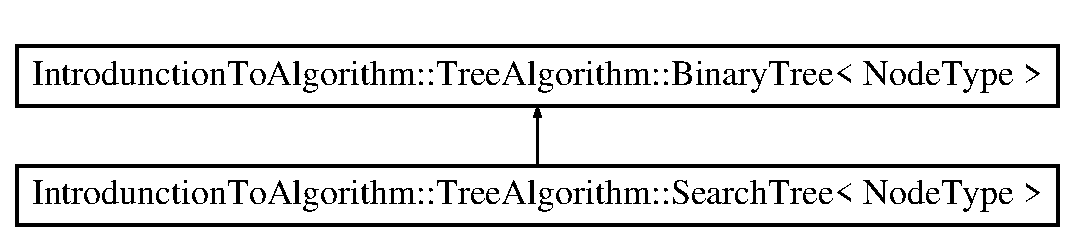
\includegraphics[height=2.000000cm]{struct_introdunction_to_algorithm_1_1_tree_algorithm_1_1_binary_tree}
\end{center}
\end{figure}
\subsection*{Public Types}
\begin{DoxyCompactItemize}
\item 
typedef Node\+Type\+::\+Key\+Type \hyperlink{struct_introdunction_to_algorithm_1_1_tree_algorithm_1_1_binary_tree_ae2feaade7bbb1e1f436475069cb1cd20}{T}
\end{DoxyCompactItemize}
\subsection*{Public Member Functions}
\begin{DoxyCompactItemize}
\item 
\hyperlink{struct_introdunction_to_algorithm_1_1_tree_algorithm_1_1_binary_tree_a32fbf1f65e0262839aa38b8eb6744781}{Binary\+Tree} ()
\begin{DoxyCompactList}\small\item\em 默认函数 \end{DoxyCompactList}\item 
std\+::string \hyperlink{struct_introdunction_to_algorithm_1_1_tree_algorithm_1_1_binary_tree_a55874f5ca046b9f3ad1d44c2f7ff4142}{to\+\_\+xml} ()
\begin{DoxyCompactList}\small\item\em to\+\_\+xml\+:返回本树的{\ttfamily xml}描述。 \end{DoxyCompactList}\end{DoxyCompactItemize}
\subsection*{Public Attributes}
\begin{DoxyCompactItemize}
\item 
std\+::shared\+\_\+ptr$<$ Node\+Type $>$ \hyperlink{struct_introdunction_to_algorithm_1_1_tree_algorithm_1_1_binary_tree_acd08e406313d41bb0dd2e17aabde8482}{root}
\end{DoxyCompactItemize}


\subsection{Detailed Description}
\subsubsection*{template$<$typename Node\+Type$>$struct Introdunction\+To\+Algorithm\+::\+Tree\+Algorithm\+::\+Binary\+Tree$<$ Node\+Type $>$}

Binary\+Tree:二叉树,算法导论10章10.4节 

二叉树通过一个root(若引用)指向一个节点对象。当root为空时,树为空 

Definition at line 13 of file binarytree.\+h.



\subsection{Member Typedef Documentation}
\hypertarget{struct_introdunction_to_algorithm_1_1_tree_algorithm_1_1_binary_tree_ae2feaade7bbb1e1f436475069cb1cd20}{}\index{Introdunction\+To\+Algorithm\+::\+Tree\+Algorithm\+::\+Binary\+Tree@{Introdunction\+To\+Algorithm\+::\+Tree\+Algorithm\+::\+Binary\+Tree}!T@{T}}
\index{T@{T}!Introdunction\+To\+Algorithm\+::\+Tree\+Algorithm\+::\+Binary\+Tree@{Introdunction\+To\+Algorithm\+::\+Tree\+Algorithm\+::\+Binary\+Tree}}
\subsubsection[{T}]{\setlength{\rightskip}{0pt plus 5cm}template$<$typename Node\+Type$>$ typedef Node\+Type\+::\+Key\+Type {\bf Introdunction\+To\+Algorithm\+::\+Tree\+Algorithm\+::\+Binary\+Tree}$<$ Node\+Type $>$\+::{\bf T}}\label{struct_introdunction_to_algorithm_1_1_tree_algorithm_1_1_binary_tree_ae2feaade7bbb1e1f436475069cb1cd20}
树的节点存储数据的类型 

Definition at line 15 of file binarytree.\+h.



\subsection{Constructor \& Destructor Documentation}
\hypertarget{struct_introdunction_to_algorithm_1_1_tree_algorithm_1_1_binary_tree_a32fbf1f65e0262839aa38b8eb6744781}{}\index{Introdunction\+To\+Algorithm\+::\+Tree\+Algorithm\+::\+Binary\+Tree@{Introdunction\+To\+Algorithm\+::\+Tree\+Algorithm\+::\+Binary\+Tree}!Binary\+Tree@{Binary\+Tree}}
\index{Binary\+Tree@{Binary\+Tree}!Introdunction\+To\+Algorithm\+::\+Tree\+Algorithm\+::\+Binary\+Tree@{Introdunction\+To\+Algorithm\+::\+Tree\+Algorithm\+::\+Binary\+Tree}}
\subsubsection[{Binary\+Tree()}]{\setlength{\rightskip}{0pt plus 5cm}template$<$typename Node\+Type$>$ {\bf Introdunction\+To\+Algorithm\+::\+Tree\+Algorithm\+::\+Binary\+Tree}$<$ Node\+Type $>$\+::{\bf Binary\+Tree} (
\begin{DoxyParamCaption}
{}
\end{DoxyParamCaption}
)\hspace{0.3cm}{\ttfamily [inline]}}\label{struct_introdunction_to_algorithm_1_1_tree_algorithm_1_1_binary_tree_a32fbf1f65e0262839aa38b8eb6744781}


默认函数 

新建的二叉树默认为空 

Definition at line 21 of file binarytree.\+h.



\subsection{Member Function Documentation}
\hypertarget{struct_introdunction_to_algorithm_1_1_tree_algorithm_1_1_binary_tree_a55874f5ca046b9f3ad1d44c2f7ff4142}{}\index{Introdunction\+To\+Algorithm\+::\+Tree\+Algorithm\+::\+Binary\+Tree@{Introdunction\+To\+Algorithm\+::\+Tree\+Algorithm\+::\+Binary\+Tree}!to\+\_\+xml@{to\+\_\+xml}}
\index{to\+\_\+xml@{to\+\_\+xml}!Introdunction\+To\+Algorithm\+::\+Tree\+Algorithm\+::\+Binary\+Tree@{Introdunction\+To\+Algorithm\+::\+Tree\+Algorithm\+::\+Binary\+Tree}}
\subsubsection[{to\+\_\+xml()}]{\setlength{\rightskip}{0pt plus 5cm}template$<$typename Node\+Type$>$ std\+::string {\bf Introdunction\+To\+Algorithm\+::\+Tree\+Algorithm\+::\+Binary\+Tree}$<$ Node\+Type $>$\+::to\+\_\+xml (
\begin{DoxyParamCaption}
{}
\end{DoxyParamCaption}
)\hspace{0.3cm}{\ttfamily [inline]}}\label{struct_introdunction_to_algorithm_1_1_tree_algorithm_1_1_binary_tree_a55874f5ca046b9f3ad1d44c2f7ff4142}


to\+\_\+xml\+:返回本树的{\ttfamily xml}描述。 

\begin{DoxyReturn}{Returns}
\+: 树的{\ttfamily xml}描述的字符串
\end{DoxyReturn}
该函数获取本树的{\ttfamily xml}描述 

Definition at line 31 of file binarytree.\+h.



\subsection{Member Data Documentation}
\hypertarget{struct_introdunction_to_algorithm_1_1_tree_algorithm_1_1_binary_tree_acd08e406313d41bb0dd2e17aabde8482}{}\index{Introdunction\+To\+Algorithm\+::\+Tree\+Algorithm\+::\+Binary\+Tree@{Introdunction\+To\+Algorithm\+::\+Tree\+Algorithm\+::\+Binary\+Tree}!root@{root}}
\index{root@{root}!Introdunction\+To\+Algorithm\+::\+Tree\+Algorithm\+::\+Binary\+Tree@{Introdunction\+To\+Algorithm\+::\+Tree\+Algorithm\+::\+Binary\+Tree}}
\subsubsection[{root}]{\setlength{\rightskip}{0pt plus 5cm}template$<$typename Node\+Type$>$ std\+::shared\+\_\+ptr$<$Node\+Type$>$ {\bf Introdunction\+To\+Algorithm\+::\+Tree\+Algorithm\+::\+Binary\+Tree}$<$ Node\+Type $>$\+::root}\label{struct_introdunction_to_algorithm_1_1_tree_algorithm_1_1_binary_tree_acd08e406313d41bb0dd2e17aabde8482}
树的根节点,时一个指向节点对象的强引用 

Definition at line 39 of file binarytree.\+h.



The documentation for this struct was generated from the following file\+:\begin{DoxyCompactItemize}
\item 
src/tree\+\_\+algorithms/binarytree/\hyperlink{binarytree_8h}{binarytree.\+h}\end{DoxyCompactItemize}

\hypertarget{struct_introdunction_to_algorithm_1_1_tree_algorithm_1_1_binary_tree_node}{}\section{Introdunction\+To\+Algorithm\+:\+:Tree\+Algorithm\+:\+:Binary\+Tree\+Node$<$ T $>$ Struct Template Reference}
\label{struct_introdunction_to_algorithm_1_1_tree_algorithm_1_1_binary_tree_node}\index{Introdunction\+To\+Algorithm\+::\+Tree\+Algorithm\+::\+Binary\+Tree\+Node$<$ T $>$@{Introdunction\+To\+Algorithm\+::\+Tree\+Algorithm\+::\+Binary\+Tree\+Node$<$ T $>$}}


Binary\+Tree\+Node:二叉树的节点,算法导论xx章xx节  




{\ttfamily \#include $<$binarytreenode.\+h$>$}

\subsection*{Public Types}
\begin{DoxyCompactItemize}
\item 
typedef T \hyperlink{struct_introdunction_to_algorithm_1_1_tree_algorithm_1_1_binary_tree_node_a0967a0c85792f7b02a005eb1942d1bf5}{Key\+Type}
\end{DoxyCompactItemize}
\subsection*{Public Member Functions}
\begin{DoxyCompactItemize}
\item 
\hyperlink{struct_introdunction_to_algorithm_1_1_tree_algorithm_1_1_binary_tree_node_a6fbeeee0c4db4b2afd3398ca5379b390}{Binary\+Tree\+Node} ()
\begin{DoxyCompactList}\small\item\em 默认构造函数 \end{DoxyCompactList}\item 
\hyperlink{struct_introdunction_to_algorithm_1_1_tree_algorithm_1_1_binary_tree_node_a511c3ca309c8e77045d360ddbba60455}{Binary\+Tree\+Node} (const T \&keyvalue)
\begin{DoxyCompactList}\small\item\em 显式构造函数 \end{DoxyCompactList}\item 
virtual std\+::string \hyperlink{struct_introdunction_to_algorithm_1_1_tree_algorithm_1_1_binary_tree_node_a85f633a95e16b767f01d3eb7a3b17997}{to\+\_\+string} ()
\begin{DoxyCompactList}\small\item\em to\+\_\+string\+:返回该节点的字符串描述 \end{DoxyCompactList}\item 
virtual std\+::string \hyperlink{struct_introdunction_to_algorithm_1_1_tree_algorithm_1_1_binary_tree_node_abefbedeac57528fcfa60cfb1728998f7}{to\+\_\+xml} ()
\begin{DoxyCompactList}\small\item\em to\+\_\+xml\+:返回以该节点为根的子树的{\ttfamily xml}描述。 \end{DoxyCompactList}\item 
bool \hyperlink{struct_introdunction_to_algorithm_1_1_tree_algorithm_1_1_binary_tree_node_a117288aa11c36d94e85664d1599c8099}{is\+\_\+left\+\_\+child} ()
\begin{DoxyCompactList}\small\item\em is\+\_\+left\+\_\+child\+:判断本节点是否左子节点。 \end{DoxyCompactList}\item 
bool \hyperlink{struct_introdunction_to_algorithm_1_1_tree_algorithm_1_1_binary_tree_node_a90c90d98b01fd0ee1060e192cd5858ef}{is\+\_\+right\+\_\+child} ()
\begin{DoxyCompactList}\small\item\em is\+\_\+right\+\_\+child\+:判断本节点是否右子节点。 \end{DoxyCompactList}\end{DoxyCompactItemize}
\subsection*{Public Attributes}
\begin{DoxyCompactItemize}
\item 
std\+::weak\+\_\+ptr$<$ \hyperlink{struct_introdunction_to_algorithm_1_1_tree_algorithm_1_1_binary_tree_node}{Binary\+Tree\+Node} $>$ \hyperlink{struct_introdunction_to_algorithm_1_1_tree_algorithm_1_1_binary_tree_node_afa42d2a3e68838d17d1028fab12c71e1}{parent}
\item 
std\+::shared\+\_\+ptr$<$ \hyperlink{struct_introdunction_to_algorithm_1_1_tree_algorithm_1_1_binary_tree_node}{Binary\+Tree\+Node} $>$ \hyperlink{struct_introdunction_to_algorithm_1_1_tree_algorithm_1_1_binary_tree_node_a3f84ee829fc539e004bf3be6eb8fb882}{lchild}
\item 
std\+::shared\+\_\+ptr$<$ \hyperlink{struct_introdunction_to_algorithm_1_1_tree_algorithm_1_1_binary_tree_node}{Binary\+Tree\+Node} $>$ \hyperlink{struct_introdunction_to_algorithm_1_1_tree_algorithm_1_1_binary_tree_node_ae6dc3c9fce595c08cd3a31dba534fec3}{rchild}
\item 
T \hyperlink{struct_introdunction_to_algorithm_1_1_tree_algorithm_1_1_binary_tree_node_a3bcf52447a097b51caa74488e90f1479}{key}
\end{DoxyCompactItemize}


\subsection{Detailed Description}
\subsubsection*{template$<$typename T$>$struct Introdunction\+To\+Algorithm\+::\+Tree\+Algorithm\+::\+Binary\+Tree\+Node$<$ T $>$}

Binary\+Tree\+Node:二叉树的节点,算法导论xx章xx节 

任何一个节点都有两个强引用指向左右子节点,以及一个弱引用指向它的父节点。节点还有一个{\ttfamily key}成员包含具体的数据 

Definition at line 13 of file binarytreenode.\+h.



\subsection{Member Typedef Documentation}
\hypertarget{struct_introdunction_to_algorithm_1_1_tree_algorithm_1_1_binary_tree_node_a0967a0c85792f7b02a005eb1942d1bf5}{}\index{Introdunction\+To\+Algorithm\+::\+Tree\+Algorithm\+::\+Binary\+Tree\+Node@{Introdunction\+To\+Algorithm\+::\+Tree\+Algorithm\+::\+Binary\+Tree\+Node}!Key\+Type@{Key\+Type}}
\index{Key\+Type@{Key\+Type}!Introdunction\+To\+Algorithm\+::\+Tree\+Algorithm\+::\+Binary\+Tree\+Node@{Introdunction\+To\+Algorithm\+::\+Tree\+Algorithm\+::\+Binary\+Tree\+Node}}
\subsubsection[{Key\+Type}]{\setlength{\rightskip}{0pt plus 5cm}template$<$typename T$>$ typedef T {\bf Introdunction\+To\+Algorithm\+::\+Tree\+Algorithm\+::\+Binary\+Tree\+Node}$<$ T $>$\+::{\bf Key\+Type}}\label{struct_introdunction_to_algorithm_1_1_tree_algorithm_1_1_binary_tree_node_a0967a0c85792f7b02a005eb1942d1bf5}
节点保存的数据的类型 

Definition at line 32 of file binarytreenode.\+h.



\subsection{Constructor \& Destructor Documentation}
\hypertarget{struct_introdunction_to_algorithm_1_1_tree_algorithm_1_1_binary_tree_node_a6fbeeee0c4db4b2afd3398ca5379b390}{}\index{Introdunction\+To\+Algorithm\+::\+Tree\+Algorithm\+::\+Binary\+Tree\+Node@{Introdunction\+To\+Algorithm\+::\+Tree\+Algorithm\+::\+Binary\+Tree\+Node}!Binary\+Tree\+Node@{Binary\+Tree\+Node}}
\index{Binary\+Tree\+Node@{Binary\+Tree\+Node}!Introdunction\+To\+Algorithm\+::\+Tree\+Algorithm\+::\+Binary\+Tree\+Node@{Introdunction\+To\+Algorithm\+::\+Tree\+Algorithm\+::\+Binary\+Tree\+Node}}
\subsubsection[{Binary\+Tree\+Node()}]{\setlength{\rightskip}{0pt plus 5cm}template$<$typename T$>$ {\bf Introdunction\+To\+Algorithm\+::\+Tree\+Algorithm\+::\+Binary\+Tree\+Node}$<$ T $>$\+::{\bf Binary\+Tree\+Node} (
\begin{DoxyParamCaption}
{}
\end{DoxyParamCaption}
)\hspace{0.3cm}{\ttfamily [inline]}}\label{struct_introdunction_to_algorithm_1_1_tree_algorithm_1_1_binary_tree_node_a6fbeeee0c4db4b2afd3398ca5379b390}


默认构造函数 

所有的成员变量都采取默认值 

Definition at line 20 of file binarytreenode.\+h.

\hypertarget{struct_introdunction_to_algorithm_1_1_tree_algorithm_1_1_binary_tree_node_a511c3ca309c8e77045d360ddbba60455}{}\index{Introdunction\+To\+Algorithm\+::\+Tree\+Algorithm\+::\+Binary\+Tree\+Node@{Introdunction\+To\+Algorithm\+::\+Tree\+Algorithm\+::\+Binary\+Tree\+Node}!Binary\+Tree\+Node@{Binary\+Tree\+Node}}
\index{Binary\+Tree\+Node@{Binary\+Tree\+Node}!Introdunction\+To\+Algorithm\+::\+Tree\+Algorithm\+::\+Binary\+Tree\+Node@{Introdunction\+To\+Algorithm\+::\+Tree\+Algorithm\+::\+Binary\+Tree\+Node}}
\subsubsection[{Binary\+Tree\+Node(const T \&keyvalue)}]{\setlength{\rightskip}{0pt plus 5cm}template$<$typename T$>$ {\bf Introdunction\+To\+Algorithm\+::\+Tree\+Algorithm\+::\+Binary\+Tree\+Node}$<$ T $>$\+::{\bf Binary\+Tree\+Node} (
\begin{DoxyParamCaption}
\item[{const T \&}]{keyvalue}
\end{DoxyParamCaption}
)\hspace{0.3cm}{\ttfamily [inline]}, {\ttfamily [explicit]}}\label{struct_introdunction_to_algorithm_1_1_tree_algorithm_1_1_binary_tree_node_a511c3ca309c8e77045d360ddbba60455}


显式构造函数 


\begin{DoxyParams}{Parameters}
{\em keyvalue\+:节点要保存的数据内容} & 指定{\ttfamily key}成员需要赋值的数据 \\
\hline
\end{DoxyParams}


Definition at line 29 of file binarytreenode.\+h.



\subsection{Member Function Documentation}
\hypertarget{struct_introdunction_to_algorithm_1_1_tree_algorithm_1_1_binary_tree_node_a117288aa11c36d94e85664d1599c8099}{}\index{Introdunction\+To\+Algorithm\+::\+Tree\+Algorithm\+::\+Binary\+Tree\+Node@{Introdunction\+To\+Algorithm\+::\+Tree\+Algorithm\+::\+Binary\+Tree\+Node}!is\+\_\+left\+\_\+child@{is\+\_\+left\+\_\+child}}
\index{is\+\_\+left\+\_\+child@{is\+\_\+left\+\_\+child}!Introdunction\+To\+Algorithm\+::\+Tree\+Algorithm\+::\+Binary\+Tree\+Node@{Introdunction\+To\+Algorithm\+::\+Tree\+Algorithm\+::\+Binary\+Tree\+Node}}
\subsubsection[{is\+\_\+left\+\_\+child()}]{\setlength{\rightskip}{0pt plus 5cm}template$<$typename T$>$ bool {\bf Introdunction\+To\+Algorithm\+::\+Tree\+Algorithm\+::\+Binary\+Tree\+Node}$<$ T $>$\+::is\+\_\+left\+\_\+child (
\begin{DoxyParamCaption}
{}
\end{DoxyParamCaption}
)\hspace{0.3cm}{\ttfamily [inline]}}\label{struct_introdunction_to_algorithm_1_1_tree_algorithm_1_1_binary_tree_node_a117288aa11c36d94e85664d1599c8099}


is\+\_\+left\+\_\+child\+:判断本节点是否左子节点。 

\begin{DoxyReturn}{Returns}
返回{\ttfamily true}或者{\ttfamily false} 该函数判断本节点是否是左子节点。如果本节点的父节点为空,则返回{\ttfamily false};如果本节点的父节点非空且本节点是父节点的左子节点,则返回{\ttfamily true};否则返回{\ttfamily false} 
\end{DoxyReturn}


Definition at line 80 of file binarytreenode.\+h.

\hypertarget{struct_introdunction_to_algorithm_1_1_tree_algorithm_1_1_binary_tree_node_a90c90d98b01fd0ee1060e192cd5858ef}{}\index{Introdunction\+To\+Algorithm\+::\+Tree\+Algorithm\+::\+Binary\+Tree\+Node@{Introdunction\+To\+Algorithm\+::\+Tree\+Algorithm\+::\+Binary\+Tree\+Node}!is\+\_\+right\+\_\+child@{is\+\_\+right\+\_\+child}}
\index{is\+\_\+right\+\_\+child@{is\+\_\+right\+\_\+child}!Introdunction\+To\+Algorithm\+::\+Tree\+Algorithm\+::\+Binary\+Tree\+Node@{Introdunction\+To\+Algorithm\+::\+Tree\+Algorithm\+::\+Binary\+Tree\+Node}}
\subsubsection[{is\+\_\+right\+\_\+child()}]{\setlength{\rightskip}{0pt plus 5cm}template$<$typename T$>$ bool {\bf Introdunction\+To\+Algorithm\+::\+Tree\+Algorithm\+::\+Binary\+Tree\+Node}$<$ T $>$\+::is\+\_\+right\+\_\+child (
\begin{DoxyParamCaption}
{}
\end{DoxyParamCaption}
)\hspace{0.3cm}{\ttfamily [inline]}}\label{struct_introdunction_to_algorithm_1_1_tree_algorithm_1_1_binary_tree_node_a90c90d98b01fd0ee1060e192cd5858ef}


is\+\_\+right\+\_\+child\+:判断本节点是否右子节点。 

\begin{DoxyReturn}{Returns}
返回{\ttfamily true}或者{\ttfamily false} 该函数判断本节点是否是右子节点。如果本节点的父节点为空,则返回{\ttfamily false};如果本节点的父节点非空且本节点是父节点的右子节点,则返回{\ttfamily true};否则返回{\ttfamily false} 
\end{DoxyReturn}


Definition at line 94 of file binarytreenode.\+h.

\hypertarget{struct_introdunction_to_algorithm_1_1_tree_algorithm_1_1_binary_tree_node_a85f633a95e16b767f01d3eb7a3b17997}{}\index{Introdunction\+To\+Algorithm\+::\+Tree\+Algorithm\+::\+Binary\+Tree\+Node@{Introdunction\+To\+Algorithm\+::\+Tree\+Algorithm\+::\+Binary\+Tree\+Node}!to\+\_\+string@{to\+\_\+string}}
\index{to\+\_\+string@{to\+\_\+string}!Introdunction\+To\+Algorithm\+::\+Tree\+Algorithm\+::\+Binary\+Tree\+Node@{Introdunction\+To\+Algorithm\+::\+Tree\+Algorithm\+::\+Binary\+Tree\+Node}}
\subsubsection[{to\+\_\+string()}]{\setlength{\rightskip}{0pt plus 5cm}template$<$typename T$>$ virtual std\+::string {\bf Introdunction\+To\+Algorithm\+::\+Tree\+Algorithm\+::\+Binary\+Tree\+Node}$<$ T $>$\+::to\+\_\+string (
\begin{DoxyParamCaption}
{}
\end{DoxyParamCaption}
)\hspace{0.3cm}{\ttfamily [inline]}, {\ttfamily [virtual]}}\label{struct_introdunction_to_algorithm_1_1_tree_algorithm_1_1_binary_tree_node_a85f633a95e16b767f01d3eb7a3b17997}


to\+\_\+string\+:返回该节点的字符串描述 

\begin{DoxyReturn}{Returns}
\+: 本节点的描述字符串
\end{DoxyReturn}
该函数打印本节点的{\ttfamily key},以及父节点(若存在)、子节点(若存在)的{\ttfamily key} 

Definition at line 39 of file binarytreenode.\+h.

\hypertarget{struct_introdunction_to_algorithm_1_1_tree_algorithm_1_1_binary_tree_node_abefbedeac57528fcfa60cfb1728998f7}{}\index{Introdunction\+To\+Algorithm\+::\+Tree\+Algorithm\+::\+Binary\+Tree\+Node@{Introdunction\+To\+Algorithm\+::\+Tree\+Algorithm\+::\+Binary\+Tree\+Node}!to\+\_\+xml@{to\+\_\+xml}}
\index{to\+\_\+xml@{to\+\_\+xml}!Introdunction\+To\+Algorithm\+::\+Tree\+Algorithm\+::\+Binary\+Tree\+Node@{Introdunction\+To\+Algorithm\+::\+Tree\+Algorithm\+::\+Binary\+Tree\+Node}}
\subsubsection[{to\+\_\+xml()}]{\setlength{\rightskip}{0pt plus 5cm}template$<$typename T$>$ virtual std\+::string {\bf Introdunction\+To\+Algorithm\+::\+Tree\+Algorithm\+::\+Binary\+Tree\+Node}$<$ T $>$\+::to\+\_\+xml (
\begin{DoxyParamCaption}
{}
\end{DoxyParamCaption}
)\hspace{0.3cm}{\ttfamily [inline]}, {\ttfamily [virtual]}}\label{struct_introdunction_to_algorithm_1_1_tree_algorithm_1_1_binary_tree_node_abefbedeac57528fcfa60cfb1728998f7}


to\+\_\+xml\+:返回以该节点为根的子树的{\ttfamily xml}描述。 

\begin{DoxyReturn}{Returns}
\+: 本节点子树的{\ttfamily xml}描述的字符串
\end{DoxyReturn}
该函数返回以本节点为根的子树的{\ttfamily xml}描述。对子节点递归调用从而生成{\ttfamily xml}数据 

Definition at line 60 of file binarytreenode.\+h.



\subsection{Member Data Documentation}
\hypertarget{struct_introdunction_to_algorithm_1_1_tree_algorithm_1_1_binary_tree_node_a3bcf52447a097b51caa74488e90f1479}{}\index{Introdunction\+To\+Algorithm\+::\+Tree\+Algorithm\+::\+Binary\+Tree\+Node@{Introdunction\+To\+Algorithm\+::\+Tree\+Algorithm\+::\+Binary\+Tree\+Node}!key@{key}}
\index{key@{key}!Introdunction\+To\+Algorithm\+::\+Tree\+Algorithm\+::\+Binary\+Tree\+Node@{Introdunction\+To\+Algorithm\+::\+Tree\+Algorithm\+::\+Binary\+Tree\+Node}}
\subsubsection[{key}]{\setlength{\rightskip}{0pt plus 5cm}template$<$typename T$>$ T {\bf Introdunction\+To\+Algorithm\+::\+Tree\+Algorithm\+::\+Binary\+Tree\+Node}$<$ T $>$\+::key}\label{struct_introdunction_to_algorithm_1_1_tree_algorithm_1_1_binary_tree_node_a3bcf52447a097b51caa74488e90f1479}
节点的保存的数据 

Definition at line 106 of file binarytreenode.\+h.

\hypertarget{struct_introdunction_to_algorithm_1_1_tree_algorithm_1_1_binary_tree_node_a3f84ee829fc539e004bf3be6eb8fb882}{}\index{Introdunction\+To\+Algorithm\+::\+Tree\+Algorithm\+::\+Binary\+Tree\+Node@{Introdunction\+To\+Algorithm\+::\+Tree\+Algorithm\+::\+Binary\+Tree\+Node}!lchild@{lchild}}
\index{lchild@{lchild}!Introdunction\+To\+Algorithm\+::\+Tree\+Algorithm\+::\+Binary\+Tree\+Node@{Introdunction\+To\+Algorithm\+::\+Tree\+Algorithm\+::\+Binary\+Tree\+Node}}
\subsubsection[{lchild}]{\setlength{\rightskip}{0pt plus 5cm}template$<$typename T$>$ std\+::shared\+\_\+ptr$<${\bf Binary\+Tree\+Node}$>$ {\bf Introdunction\+To\+Algorithm\+::\+Tree\+Algorithm\+::\+Binary\+Tree\+Node}$<$ T $>$\+::lchild}\label{struct_introdunction_to_algorithm_1_1_tree_algorithm_1_1_binary_tree_node_a3f84ee829fc539e004bf3be6eb8fb882}
节点的左子节点的强引用 

Definition at line 104 of file binarytreenode.\+h.

\hypertarget{struct_introdunction_to_algorithm_1_1_tree_algorithm_1_1_binary_tree_node_afa42d2a3e68838d17d1028fab12c71e1}{}\index{Introdunction\+To\+Algorithm\+::\+Tree\+Algorithm\+::\+Binary\+Tree\+Node@{Introdunction\+To\+Algorithm\+::\+Tree\+Algorithm\+::\+Binary\+Tree\+Node}!parent@{parent}}
\index{parent@{parent}!Introdunction\+To\+Algorithm\+::\+Tree\+Algorithm\+::\+Binary\+Tree\+Node@{Introdunction\+To\+Algorithm\+::\+Tree\+Algorithm\+::\+Binary\+Tree\+Node}}
\subsubsection[{parent}]{\setlength{\rightskip}{0pt plus 5cm}template$<$typename T$>$ std\+::weak\+\_\+ptr$<${\bf Binary\+Tree\+Node}$>$ {\bf Introdunction\+To\+Algorithm\+::\+Tree\+Algorithm\+::\+Binary\+Tree\+Node}$<$ T $>$\+::parent}\label{struct_introdunction_to_algorithm_1_1_tree_algorithm_1_1_binary_tree_node_afa42d2a3e68838d17d1028fab12c71e1}
节点的父节点的弱引用 

Definition at line 103 of file binarytreenode.\+h.

\hypertarget{struct_introdunction_to_algorithm_1_1_tree_algorithm_1_1_binary_tree_node_ae6dc3c9fce595c08cd3a31dba534fec3}{}\index{Introdunction\+To\+Algorithm\+::\+Tree\+Algorithm\+::\+Binary\+Tree\+Node@{Introdunction\+To\+Algorithm\+::\+Tree\+Algorithm\+::\+Binary\+Tree\+Node}!rchild@{rchild}}
\index{rchild@{rchild}!Introdunction\+To\+Algorithm\+::\+Tree\+Algorithm\+::\+Binary\+Tree\+Node@{Introdunction\+To\+Algorithm\+::\+Tree\+Algorithm\+::\+Binary\+Tree\+Node}}
\subsubsection[{rchild}]{\setlength{\rightskip}{0pt plus 5cm}template$<$typename T$>$ std\+::shared\+\_\+ptr$<${\bf Binary\+Tree\+Node}$>$ {\bf Introdunction\+To\+Algorithm\+::\+Tree\+Algorithm\+::\+Binary\+Tree\+Node}$<$ T $>$\+::rchild}\label{struct_introdunction_to_algorithm_1_1_tree_algorithm_1_1_binary_tree_node_ae6dc3c9fce595c08cd3a31dba534fec3}
节点的右子节点的强引用 

Definition at line 105 of file binarytreenode.\+h.



The documentation for this struct was generated from the following file\+:\begin{DoxyCompactItemize}
\item 
src/tree\+\_\+algorithms/binarytreenode/\hyperlink{binarytreenode_8h}{binarytreenode.\+h}\end{DoxyCompactItemize}

\hypertarget{class_binary_tree_test}{}\section{Binary\+Tree\+Test Class Reference}
\label{class_binary_tree_test}\index{Binary\+Tree\+Test@{Binary\+Tree\+Test}}


\hyperlink{class_binary_tree_test}{Binary\+Tree\+Test}\+:测试类,用于为测试提供基础数据  




{\ttfamily \#include $<$binarytree\+\_\+test.\+h$>$}

Inheritance diagram for Binary\+Tree\+Test\+:\begin{figure}[H]
\begin{center}
\leavevmode
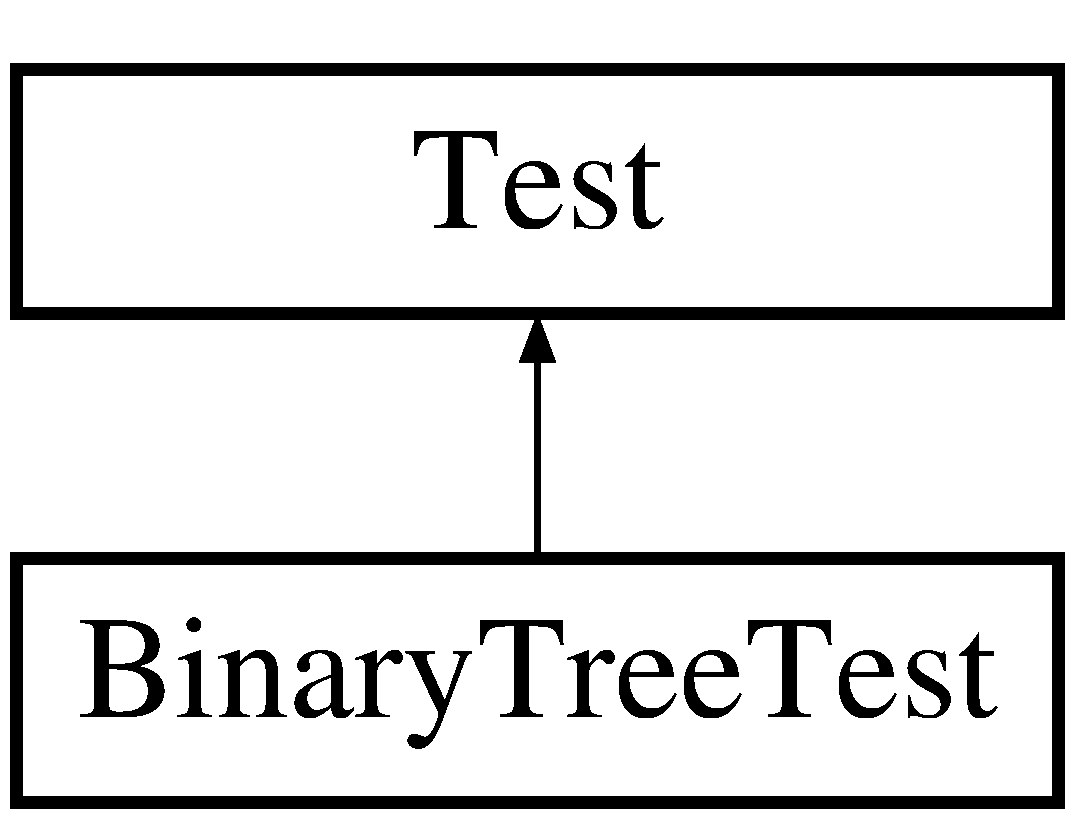
\includegraphics[height=2.000000cm]{class_binary_tree_test}
\end{center}
\end{figure}
\subsection*{Public Types}
\begin{DoxyCompactItemize}
\item 
typedef \hyperlink{struct_introdunction_to_algorithm_1_1_tree_algorithm_1_1_binary_tree_node}{Binary\+Tree\+Node}$<$ int $>$ \hyperlink{class_binary_tree_test_ad4aa3d3d01bf0b1b820fffa58e81e15b}{Node}
\end{DoxyCompactItemize}
\subsection*{Protected Member Functions}
\begin{DoxyCompactItemize}
\item 
\hyperlink{class_binary_tree_test_ab650cb6b7b008479f5294b1ed65871e5}{Binary\+Tree\+Test} ()
\item 
void \hyperlink{class_binary_tree_test_ab718ba725e8099dda414f5dbc11e881b}{Set\+Up} ()
\begin{DoxyCompactList}\small\item\em Set\+Up\+:在每一个测试开始之前执行 \end{DoxyCompactList}\item 
void \hyperlink{class_binary_tree_test_ac8daf6a6b88e89733c0ade6da7d4a897}{Tear\+Down} ()
\begin{DoxyCompactList}\small\item\em Tear\+Down\+:在每一个测试结束之后执行 \end{DoxyCompactList}\end{DoxyCompactItemize}
\subsection*{Protected Attributes}
\begin{DoxyCompactItemize}
\item 
\hyperlink{struct_introdunction_to_algorithm_1_1_tree_algorithm_1_1_binary_tree}{Binary\+Tree}$<$ \hyperlink{class_binary_tree_test_ad4aa3d3d01bf0b1b820fffa58e81e15b}{Node} $>$ \hyperlink{class_binary_tree_test_a66e48418e5449b663b2608f4914100d5}{\+\_\+empty\+\_\+tree}
\item 
\hyperlink{struct_introdunction_to_algorithm_1_1_tree_algorithm_1_1_binary_tree}{Binary\+Tree}$<$ \hyperlink{class_binary_tree_test_ad4aa3d3d01bf0b1b820fffa58e81e15b}{Node} $>$ \hyperlink{class_binary_tree_test_a36a98db1094f92c94b7d7893c8975f57}{\+\_\+normal\+\_\+tree}
\end{DoxyCompactItemize}


\subsection{Detailed Description}
\hyperlink{class_binary_tree_test}{Binary\+Tree\+Test}\+:测试类,用于为测试提供基础数据 

{\ttfamily \hyperlink{class_binary_tree_test}{Binary\+Tree\+Test}}是 {\ttfamily \+::testing\+::\+Test} 的子类。它主要用于为每一个{\ttfamily T\+E\+S\+T\+\_\+\+F}准备测试环境 

Definition at line 18 of file binarytree\+\_\+test.\+h.



\subsection{Member Typedef Documentation}
\hypertarget{class_binary_tree_test_ad4aa3d3d01bf0b1b820fffa58e81e15b}{}\index{Binary\+Tree\+Test@{Binary\+Tree\+Test}!Node@{Node}}
\index{Node@{Node}!Binary\+Tree\+Test@{Binary\+Tree\+Test}}
\subsubsection[{Node}]{\setlength{\rightskip}{0pt plus 5cm}typedef {\bf Binary\+Tree\+Node}$<$int$>$ {\bf Binary\+Tree\+Test\+::\+Node}}\label{class_binary_tree_test_ad4aa3d3d01bf0b1b820fffa58e81e15b}


Definition at line 21 of file binarytree\+\_\+test.\+h.



\subsection{Constructor \& Destructor Documentation}
\hypertarget{class_binary_tree_test_ab650cb6b7b008479f5294b1ed65871e5}{}\index{Binary\+Tree\+Test@{Binary\+Tree\+Test}!Binary\+Tree\+Test@{Binary\+Tree\+Test}}
\index{Binary\+Tree\+Test@{Binary\+Tree\+Test}!Binary\+Tree\+Test@{Binary\+Tree\+Test}}
\subsubsection[{Binary\+Tree\+Test()}]{\setlength{\rightskip}{0pt plus 5cm}Binary\+Tree\+Test\+::\+Binary\+Tree\+Test (
\begin{DoxyParamCaption}
{}
\end{DoxyParamCaption}
)\hspace{0.3cm}{\ttfamily [inline]}, {\ttfamily [protected]}}\label{class_binary_tree_test_ab650cb6b7b008479f5294b1ed65871e5}


Definition at line 23 of file binarytree\+\_\+test.\+h.



\subsection{Member Function Documentation}
\hypertarget{class_binary_tree_test_ab718ba725e8099dda414f5dbc11e881b}{}\index{Binary\+Tree\+Test@{Binary\+Tree\+Test}!Set\+Up@{Set\+Up}}
\index{Set\+Up@{Set\+Up}!Binary\+Tree\+Test@{Binary\+Tree\+Test}}
\subsubsection[{Set\+Up()}]{\setlength{\rightskip}{0pt plus 5cm}void Binary\+Tree\+Test\+::\+Set\+Up (
\begin{DoxyParamCaption}
{}
\end{DoxyParamCaption}
)\hspace{0.3cm}{\ttfamily [inline]}, {\ttfamily [protected]}}\label{class_binary_tree_test_ab718ba725e8099dda414f5dbc11e881b}


Set\+Up\+:在每一个测试开始之前执行 

{\ttfamily Set\+Up}是 {\ttfamily \+::testing\+::\+Test} 的的虚函数。它主要用于为每一个测试提供测试环境 

Definition at line 30 of file binarytree\+\_\+test.\+h.

\hypertarget{class_binary_tree_test_ac8daf6a6b88e89733c0ade6da7d4a897}{}\index{Binary\+Tree\+Test@{Binary\+Tree\+Test}!Tear\+Down@{Tear\+Down}}
\index{Tear\+Down@{Tear\+Down}!Binary\+Tree\+Test@{Binary\+Tree\+Test}}
\subsubsection[{Tear\+Down()}]{\setlength{\rightskip}{0pt plus 5cm}void Binary\+Tree\+Test\+::\+Tear\+Down (
\begin{DoxyParamCaption}
{}
\end{DoxyParamCaption}
)\hspace{0.3cm}{\ttfamily [inline]}, {\ttfamily [protected]}}\label{class_binary_tree_test_ac8daf6a6b88e89733c0ade6da7d4a897}


Tear\+Down\+:在每一个测试结束之后执行 

{\ttfamily Tear\+Down}是 {\ttfamily \+::testing\+::\+Test} 的的虚函数。它主要用于为每个测试销毁测试环境 

Definition at line 70 of file binarytree\+\_\+test.\+h.



\subsection{Member Data Documentation}
\hypertarget{class_binary_tree_test_a66e48418e5449b663b2608f4914100d5}{}\index{Binary\+Tree\+Test@{Binary\+Tree\+Test}!\+\_\+empty\+\_\+tree@{\+\_\+empty\+\_\+tree}}
\index{\+\_\+empty\+\_\+tree@{\+\_\+empty\+\_\+tree}!Binary\+Tree\+Test@{Binary\+Tree\+Test}}
\subsubsection[{\+\_\+empty\+\_\+tree}]{\setlength{\rightskip}{0pt plus 5cm}{\bf Binary\+Tree}$<${\bf Node}$>$ Binary\+Tree\+Test\+::\+\_\+empty\+\_\+tree\hspace{0.3cm}{\ttfamily [protected]}}\label{class_binary_tree_test_a66e48418e5449b663b2608f4914100d5}
一个空的树 

Definition at line 72 of file binarytree\+\_\+test.\+h.

\hypertarget{class_binary_tree_test_a36a98db1094f92c94b7d7893c8975f57}{}\index{Binary\+Tree\+Test@{Binary\+Tree\+Test}!\+\_\+normal\+\_\+tree@{\+\_\+normal\+\_\+tree}}
\index{\+\_\+normal\+\_\+tree@{\+\_\+normal\+\_\+tree}!Binary\+Tree\+Test@{Binary\+Tree\+Test}}
\subsubsection[{\+\_\+normal\+\_\+tree}]{\setlength{\rightskip}{0pt plus 5cm}{\bf Binary\+Tree}$<${\bf Node}$>$ Binary\+Tree\+Test\+::\+\_\+normal\+\_\+tree\hspace{0.3cm}{\ttfamily [protected]}}\label{class_binary_tree_test_a36a98db1094f92c94b7d7893c8975f57}
一个非空的数 

Definition at line 73 of file binarytree\+\_\+test.\+h.



The documentation for this class was generated from the following file\+:\begin{DoxyCompactItemize}
\item 
src/tree\+\_\+algorithms/binarytree/\hyperlink{binarytree__test_8h}{binarytree\+\_\+test.\+h}\end{DoxyCompactItemize}

\hypertarget{class_introdunction_to_algorithm_1_1_tree_algorithm_1_1_search_tree}{}\section{Introdunction\+To\+Algorithm\+:\+:Tree\+Algorithm\+:\+:Search\+Tree$<$ Node\+Type $>$ Class Template Reference}
\label{class_introdunction_to_algorithm_1_1_tree_algorithm_1_1_search_tree}\index{Introdunction\+To\+Algorithm\+::\+Tree\+Algorithm\+::\+Search\+Tree$<$ Node\+Type $>$@{Introdunction\+To\+Algorithm\+::\+Tree\+Algorithm\+::\+Search\+Tree$<$ Node\+Type $>$}}


Search\+Tree:二叉搜索树,算法导论12章  




{\ttfamily \#include $<$searchtree.\+h$>$}

Inheritance diagram for Introdunction\+To\+Algorithm\+:\+:Tree\+Algorithm\+:\+:Search\+Tree$<$ Node\+Type $>$\+:\begin{figure}[H]
\begin{center}
\leavevmode
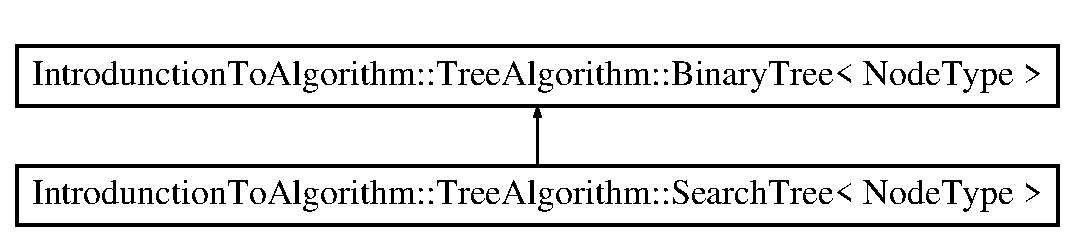
\includegraphics[height=2.000000cm]{class_introdunction_to_algorithm_1_1_tree_algorithm_1_1_search_tree}
\end{center}
\end{figure}
\subsection*{Public Types}
\begin{DoxyCompactItemize}
\item 
typedef Node\+Type\+::\+Key\+Type \hyperlink{class_introdunction_to_algorithm_1_1_tree_algorithm_1_1_search_tree_a455a92d072da5c55c969cdfc0e71ac2e}{T}
\end{DoxyCompactItemize}
\subsection*{Public Member Functions}
\begin{DoxyCompactItemize}
\item 
std\+::shared\+\_\+ptr$<$ Node\+Type $>$ \hyperlink{class_introdunction_to_algorithm_1_1_tree_algorithm_1_1_search_tree_a55d663befd7f7ef9d2238963666c69ff}{search} (const \hyperlink{struct_introdunction_to_algorithm_1_1_tree_algorithm_1_1_binary_tree_ae2feaade7bbb1e1f436475069cb1cd20}{T} \&value, std\+::shared\+\_\+ptr$<$ Node\+Type $>$ node=std\+::shared\+\_\+ptr$<$ Node\+Type $>$())
\begin{DoxyCompactList}\small\item\em search\+:在二叉搜索树中搜索指定内容的节点。 \end{DoxyCompactList}\item 
std\+::shared\+\_\+ptr$<$ Node\+Type $>$ \hyperlink{class_introdunction_to_algorithm_1_1_tree_algorithm_1_1_search_tree_a8e649931312fb7a65828e6f6e42bca41}{min} (std\+::shared\+\_\+ptr$<$ Node\+Type $>$ node)
\begin{DoxyCompactList}\small\item\em min\+:在二叉搜索树中最小值的节点。 \end{DoxyCompactList}\item 
std\+::shared\+\_\+ptr$<$ Node\+Type $>$ \hyperlink{class_introdunction_to_algorithm_1_1_tree_algorithm_1_1_search_tree_af10c9358b2e5eee2da3badac45c83575}{max} (std\+::shared\+\_\+ptr$<$ Node\+Type $>$ node)
\begin{DoxyCompactList}\small\item\em max\+:在二叉搜索树中最大值的节点。 \end{DoxyCompactList}\item 
std\+::shared\+\_\+ptr$<$ Node\+Type $>$ \hyperlink{class_introdunction_to_algorithm_1_1_tree_algorithm_1_1_search_tree_ab45b77621f5a621eaf41cf632d11e330}{successor} (std\+::shared\+\_\+ptr$<$ Node\+Type $>$ node)
\begin{DoxyCompactList}\small\item\em successor\+:二叉搜索树指定节点的后继节点。 \end{DoxyCompactList}\item 
std\+::shared\+\_\+ptr$<$ Node\+Type $>$ \hyperlink{class_introdunction_to_algorithm_1_1_tree_algorithm_1_1_search_tree_a9ee0a812fc758a4be7c0674b1549b32e}{predecesor} (std\+::shared\+\_\+ptr$<$ Node\+Type $>$ node)
\begin{DoxyCompactList}\small\item\em predecesor\+:二叉搜索树指定节点的前驱。 \end{DoxyCompactList}\item 
void \hyperlink{class_introdunction_to_algorithm_1_1_tree_algorithm_1_1_search_tree_aa65abd78c422c5162804932dc9b47ae7}{insert} (std\+::shared\+\_\+ptr$<$ Node\+Type $>$ node)
\begin{DoxyCompactList}\small\item\em insert\+:向二叉搜索树中插入节点。 \end{DoxyCompactList}\item 
void \hyperlink{class_introdunction_to_algorithm_1_1_tree_algorithm_1_1_search_tree_a80dffa04b166dbb9c04c97ea5b42dfc9}{remove} (std\+::shared\+\_\+ptr$<$ Node\+Type $>$ node)
\begin{DoxyCompactList}\small\item\em remove\+:从二叉搜索树中删除节点。 \end{DoxyCompactList}\end{DoxyCompactItemize}
\subsection*{Additional Inherited Members}


\subsection{Detailed Description}
\subsubsection*{template$<$typename Node\+Type$>$class Introdunction\+To\+Algorithm\+::\+Tree\+Algorithm\+::\+Search\+Tree$<$ Node\+Type $>$}

Search\+Tree:二叉搜索树,算法导论12章 

二叉搜索树是一种特殊的二叉树。在二叉树中的任何一个节点,该节点的左子节点值小于它;该节点的右子节点值大于它。

\begin{quote}
这里节点值指的是节点存储的数据的值\end{quote}


Definition at line 15 of file searchtree.\+h.



\subsection{Member Typedef Documentation}
\hypertarget{class_introdunction_to_algorithm_1_1_tree_algorithm_1_1_search_tree_a455a92d072da5c55c969cdfc0e71ac2e}{}\index{Introdunction\+To\+Algorithm\+::\+Tree\+Algorithm\+::\+Search\+Tree@{Introdunction\+To\+Algorithm\+::\+Tree\+Algorithm\+::\+Search\+Tree}!T@{T}}
\index{T@{T}!Introdunction\+To\+Algorithm\+::\+Tree\+Algorithm\+::\+Search\+Tree@{Introdunction\+To\+Algorithm\+::\+Tree\+Algorithm\+::\+Search\+Tree}}
\subsubsection[{T}]{\setlength{\rightskip}{0pt plus 5cm}template$<$typename Node\+Type$>$ typedef Node\+Type\+::\+Key\+Type {\bf Introdunction\+To\+Algorithm\+::\+Tree\+Algorithm\+::\+Search\+Tree}$<$ Node\+Type $>$\+::{\bf T}}\label{class_introdunction_to_algorithm_1_1_tree_algorithm_1_1_search_tree_a455a92d072da5c55c969cdfc0e71ac2e}
树的节点存储数据的类型 

Definition at line 18 of file searchtree.\+h.



\subsection{Member Function Documentation}
\hypertarget{class_introdunction_to_algorithm_1_1_tree_algorithm_1_1_search_tree_aa65abd78c422c5162804932dc9b47ae7}{}\index{Introdunction\+To\+Algorithm\+::\+Tree\+Algorithm\+::\+Search\+Tree@{Introdunction\+To\+Algorithm\+::\+Tree\+Algorithm\+::\+Search\+Tree}!insert@{insert}}
\index{insert@{insert}!Introdunction\+To\+Algorithm\+::\+Tree\+Algorithm\+::\+Search\+Tree@{Introdunction\+To\+Algorithm\+::\+Tree\+Algorithm\+::\+Search\+Tree}}
\subsubsection[{insert(std\+::shared\+\_\+ptr$<$ Node\+Type $>$ node)}]{\setlength{\rightskip}{0pt plus 5cm}template$<$typename Node\+Type$>$ void {\bf Introdunction\+To\+Algorithm\+::\+Tree\+Algorithm\+::\+Search\+Tree}$<$ Node\+Type $>$\+::insert (
\begin{DoxyParamCaption}
\item[{std\+::shared\+\_\+ptr$<$ Node\+Type $>$}]{node}
\end{DoxyParamCaption}
)\hspace{0.3cm}{\ttfamily [inline]}}\label{class_introdunction_to_algorithm_1_1_tree_algorithm_1_1_search_tree_aa65abd78c422c5162804932dc9b47ae7}


insert\+:向二叉搜索树中插入节点。 


\begin{DoxyParams}{Parameters}
{\em node\+:要插入的节点} & \\
\hline
\end{DoxyParams}
\begin{DoxyReturn}{Returns}
\+: void
\end{DoxyReturn}
给定新节点{\ttfamily node},将该节点插入到二叉搜索树中。

算法:遍历二叉搜索树,若当前节点的值大于{\ttfamily node}的值,则向左侧遍历;若当前节点值小于{\ttfamily node}的值,则向右侧遍历。直到碰到{\ttfamily nullptr}则挂载该节点

算法时间复杂度\+O(h),空间复杂度\+O(1)。其中h为树的高度 

Definition at line 173 of file searchtree.\+h.

\hypertarget{class_introdunction_to_algorithm_1_1_tree_algorithm_1_1_search_tree_af10c9358b2e5eee2da3badac45c83575}{}\index{Introdunction\+To\+Algorithm\+::\+Tree\+Algorithm\+::\+Search\+Tree@{Introdunction\+To\+Algorithm\+::\+Tree\+Algorithm\+::\+Search\+Tree}!max@{max}}
\index{max@{max}!Introdunction\+To\+Algorithm\+::\+Tree\+Algorithm\+::\+Search\+Tree@{Introdunction\+To\+Algorithm\+::\+Tree\+Algorithm\+::\+Search\+Tree}}
\subsubsection[{max(std\+::shared\+\_\+ptr$<$ Node\+Type $>$ node)}]{\setlength{\rightskip}{0pt plus 5cm}template$<$typename Node\+Type$>$ std\+::shared\+\_\+ptr$<$Node\+Type$>$ {\bf Introdunction\+To\+Algorithm\+::\+Tree\+Algorithm\+::\+Search\+Tree}$<$ Node\+Type $>$\+::max (
\begin{DoxyParamCaption}
\item[{std\+::shared\+\_\+ptr$<$ Node\+Type $>$}]{node}
\end{DoxyParamCaption}
)\hspace{0.3cm}{\ttfamily [inline]}}\label{class_introdunction_to_algorithm_1_1_tree_algorithm_1_1_search_tree_af10c9358b2e5eee2da3badac45c83575}


max\+:在二叉搜索树中最大值的节点。 


\begin{DoxyParams}{Parameters}
{\em node\+:从指定节点开始搜索(默认为树的根节点)} & \\
\hline
\end{DoxyParams}
\begin{DoxyReturn}{Returns}
\+: 二叉树种的最大节点的强引用
\end{DoxyReturn}
在二叉搜索树中搜索最小值的节点。其中可以指定从哪个节点开始搜索。若不指定搜索节点,则默认为树的根节点

算法:由于二叉树的性质,搜索最大值很简单。从指定节点沿着右子节点一路向下遍历,最右下方的节点即为最小值节点

算法时间复杂度\+O(h),空间复杂度\+O(1)。其中h为树的高度 

Definition at line 81 of file searchtree.\+h.

\hypertarget{class_introdunction_to_algorithm_1_1_tree_algorithm_1_1_search_tree_a8e649931312fb7a65828e6f6e42bca41}{}\index{Introdunction\+To\+Algorithm\+::\+Tree\+Algorithm\+::\+Search\+Tree@{Introdunction\+To\+Algorithm\+::\+Tree\+Algorithm\+::\+Search\+Tree}!min@{min}}
\index{min@{min}!Introdunction\+To\+Algorithm\+::\+Tree\+Algorithm\+::\+Search\+Tree@{Introdunction\+To\+Algorithm\+::\+Tree\+Algorithm\+::\+Search\+Tree}}
\subsubsection[{min(std\+::shared\+\_\+ptr$<$ Node\+Type $>$ node)}]{\setlength{\rightskip}{0pt plus 5cm}template$<$typename Node\+Type$>$ std\+::shared\+\_\+ptr$<$Node\+Type$>$ {\bf Introdunction\+To\+Algorithm\+::\+Tree\+Algorithm\+::\+Search\+Tree}$<$ Node\+Type $>$\+::min (
\begin{DoxyParamCaption}
\item[{std\+::shared\+\_\+ptr$<$ Node\+Type $>$}]{node}
\end{DoxyParamCaption}
)\hspace{0.3cm}{\ttfamily [inline]}}\label{class_introdunction_to_algorithm_1_1_tree_algorithm_1_1_search_tree_a8e649931312fb7a65828e6f6e42bca41}


min\+:在二叉搜索树中最小值的节点。 


\begin{DoxyParams}{Parameters}
{\em node\+:从指定节点开始搜索(默认为树的根节点)} & \\
\hline
\end{DoxyParams}
\begin{DoxyReturn}{Returns}
\+: 二叉树种的最小节点的强引用
\end{DoxyReturn}
在二叉搜索树中搜索最小值的节点。其中可以指定从哪个节点开始搜索。若不指定搜索节点,则默认为树的根节点。

算法:由于二叉树的性质,搜索最小值很简单。从指定节点沿着左子节点一路向下遍历,最左下方的节点即为最小值节点

算法时间复杂度\+O(h),空间复杂度\+O(1)。其中h为树的高度 

Definition at line 57 of file searchtree.\+h.

\hypertarget{class_introdunction_to_algorithm_1_1_tree_algorithm_1_1_search_tree_a9ee0a812fc758a4be7c0674b1549b32e}{}\index{Introdunction\+To\+Algorithm\+::\+Tree\+Algorithm\+::\+Search\+Tree@{Introdunction\+To\+Algorithm\+::\+Tree\+Algorithm\+::\+Search\+Tree}!predecesor@{predecesor}}
\index{predecesor@{predecesor}!Introdunction\+To\+Algorithm\+::\+Tree\+Algorithm\+::\+Search\+Tree@{Introdunction\+To\+Algorithm\+::\+Tree\+Algorithm\+::\+Search\+Tree}}
\subsubsection[{predecesor(std\+::shared\+\_\+ptr$<$ Node\+Type $>$ node)}]{\setlength{\rightskip}{0pt plus 5cm}template$<$typename Node\+Type$>$ std\+::shared\+\_\+ptr$<$Node\+Type$>$ {\bf Introdunction\+To\+Algorithm\+::\+Tree\+Algorithm\+::\+Search\+Tree}$<$ Node\+Type $>$\+::predecesor (
\begin{DoxyParamCaption}
\item[{std\+::shared\+\_\+ptr$<$ Node\+Type $>$}]{node}
\end{DoxyParamCaption}
)\hspace{0.3cm}{\ttfamily [inline]}}\label{class_introdunction_to_algorithm_1_1_tree_algorithm_1_1_search_tree_a9ee0a812fc758a4be7c0674b1549b32e}


predecesor\+:二叉搜索树指定节点的前驱。 


\begin{DoxyParams}{Parameters}
{\em node\+:要搜索前驱的节点} & \\
\hline
\end{DoxyParams}
\begin{DoxyReturn}{Returns}
\+: 该节点的前驱节点的强引用或者空
\end{DoxyReturn}
给定二叉搜索树的某个节点,搜索其前驱节点。所谓的某节点{\ttfamily node}的前驱节点就是在二叉搜索树中,值小于{\ttfamily node}的所有节点中最大的那一个。

一个节点{\ttfamily node}的前驱有以下情况:


\begin{DoxyItemize}
\item 如果{\ttfamily node}有左子节点,则以左子节点为根的子树中的最大值节点就是{\ttfamily node}的前驱节点
\item 如果{\ttfamily node}没有左子节点,则查看父节点
\begin{DoxyItemize}
\item 若{\ttfamily node}是父节点的右子节点;则{\ttfamily node}的前驱节点是{\ttfamily node}的父节点
\item 若{\ttfamily node}是父节点的左子节点;则{\ttfamily node}设置为{\ttfamily node-\/$>$parent},递归向直到{\ttfamily node}是它父亲的右子节点;此时{\ttfamily node}的前驱节点是{\ttfamily node}的父节点
\end{DoxyItemize}
\end{DoxyItemize}

算法时间复杂度\+O(h),空间复杂度\+O(1)。其中h为树的高度 

Definition at line 143 of file searchtree.\+h.

\hypertarget{class_introdunction_to_algorithm_1_1_tree_algorithm_1_1_search_tree_a80dffa04b166dbb9c04c97ea5b42dfc9}{}\index{Introdunction\+To\+Algorithm\+::\+Tree\+Algorithm\+::\+Search\+Tree@{Introdunction\+To\+Algorithm\+::\+Tree\+Algorithm\+::\+Search\+Tree}!remove@{remove}}
\index{remove@{remove}!Introdunction\+To\+Algorithm\+::\+Tree\+Algorithm\+::\+Search\+Tree@{Introdunction\+To\+Algorithm\+::\+Tree\+Algorithm\+::\+Search\+Tree}}
\subsubsection[{remove(std\+::shared\+\_\+ptr$<$ Node\+Type $>$ node)}]{\setlength{\rightskip}{0pt plus 5cm}template$<$typename Node\+Type$>$ void {\bf Introdunction\+To\+Algorithm\+::\+Tree\+Algorithm\+::\+Search\+Tree}$<$ Node\+Type $>$\+::remove (
\begin{DoxyParamCaption}
\item[{std\+::shared\+\_\+ptr$<$ Node\+Type $>$}]{node}
\end{DoxyParamCaption}
)\hspace{0.3cm}{\ttfamily [inline]}}\label{class_introdunction_to_algorithm_1_1_tree_algorithm_1_1_search_tree_a80dffa04b166dbb9c04c97ea5b42dfc9}


remove\+:从二叉搜索树中删除节点。 


\begin{DoxyParams}{Parameters}
{\em node\+:要删除的节点} & \\
\hline
\end{DoxyParams}
\begin{DoxyReturn}{Returns}
\+: void
\end{DoxyReturn}
给定节点{\ttfamily node},从二叉搜索树中删除它。如果{\ttfamily node}不在二叉搜索树中则抛出异常。

算法:


\begin{DoxyItemize}
\item 如果{\ttfamily node}是一个叶子节点:则直接删除它
\item 如果{\ttfamily node}有左子节点,但是没有右子节点:将左子剪切到{\ttfamily node}所在位置
\item 如果{\ttfamily node}有右子节点,但是没有左子节点:将右子剪切到{\ttfamily node}所在位置
\item 如果{\ttfamily node}既有左子节点,又有右子节点:首先获取{\ttfamily node}的后继节点{\ttfamily next\+\_\+node}
\begin{DoxyItemize}
\item 如果{\ttfamily next\+\_\+node}就是{\ttfamily node}的右子节点,则证明{\ttfamily next\+\_\+node}没有左子(如果{\ttfamily next\+\_\+node}有左子,则{\ttfamily node}的后继节点必然不是{\ttfamily next\+\_\+node})。 此时将{\ttfamily next\+\_\+node}剪切到{\ttfamily node}所在位置,并且将{\ttfamily node}的左子挂载到{\ttfamily next\+\_\+node}的左子
\item 如果{\ttfamily next\+\_\+node}不是{\ttfamily node}的右子节点,则{\ttfamily next\+\_\+node}必然位于{\ttfamily node}右子为根的子树中。且{\ttfamily next\+\_\+node}必然没有左子(否则{\ttfamily node}的后继节点必然不是{\ttfamily next\+\_\+node})
\begin{DoxyItemize}
\item 把{\ttfamily next\+\_\+node}的右子节点剪切到{\ttfamily next\+\_\+node}的位置
\item 将{\ttfamily next\+\_\+node}剪切到{\ttfamily node}的右子位置
\item 执行{\ttfamily next\+\_\+node}就是{\ttfamily node}的右子节点的操作
\end{DoxyItemize}
\end{DoxyItemize}
\end{DoxyItemize}

算法时间复杂度\+O(h),空间复杂度\+O(1)。其中h为树的高度 

Definition at line 232 of file searchtree.\+h.

\hypertarget{class_introdunction_to_algorithm_1_1_tree_algorithm_1_1_search_tree_a55d663befd7f7ef9d2238963666c69ff}{}\index{Introdunction\+To\+Algorithm\+::\+Tree\+Algorithm\+::\+Search\+Tree@{Introdunction\+To\+Algorithm\+::\+Tree\+Algorithm\+::\+Search\+Tree}!search@{search}}
\index{search@{search}!Introdunction\+To\+Algorithm\+::\+Tree\+Algorithm\+::\+Search\+Tree@{Introdunction\+To\+Algorithm\+::\+Tree\+Algorithm\+::\+Search\+Tree}}
\subsubsection[{search(const T \&value, std\+::shared\+\_\+ptr$<$ Node\+Type $>$ node=std\+::shared\+\_\+ptr$<$ Node\+Type $>$())}]{\setlength{\rightskip}{0pt plus 5cm}template$<$typename Node\+Type$>$ std\+::shared\+\_\+ptr$<$Node\+Type$>$ {\bf Introdunction\+To\+Algorithm\+::\+Tree\+Algorithm\+::\+Search\+Tree}$<$ Node\+Type $>$\+::search (
\begin{DoxyParamCaption}
\item[{const {\bf T} \&}]{value, }
\item[{std\+::shared\+\_\+ptr$<$ Node\+Type $>$}]{node = {\ttfamily std\+:\+:shared\+\_\+ptr$<$NodeType$>$()}}
\end{DoxyParamCaption}
)\hspace{0.3cm}{\ttfamily [inline]}}\label{class_introdunction_to_algorithm_1_1_tree_algorithm_1_1_search_tree_a55d663befd7f7ef9d2238963666c69ff}


search\+:在二叉搜索树中搜索指定内容的节点。 


\begin{DoxyParams}{Parameters}
{\em value} & 搜索指定的内容 \\
\hline
{\em node\+:从指定节点开始搜索(默认为树的根节点)} & \\
\hline
\end{DoxyParams}
\begin{DoxyReturn}{Returns}
\+: 存储内容等于value的节点的强引用或者空
\end{DoxyReturn}
在二叉搜索树中搜索指定内容的节点。其中可以指定从哪个节点开始搜索。若不指定搜索节点,则默认为树的根节点.

算法时间复杂度\+O(h),空间复杂度\+O(1)。其中h为树的高度 

Definition at line 30 of file searchtree.\+h.

\hypertarget{class_introdunction_to_algorithm_1_1_tree_algorithm_1_1_search_tree_ab45b77621f5a621eaf41cf632d11e330}{}\index{Introdunction\+To\+Algorithm\+::\+Tree\+Algorithm\+::\+Search\+Tree@{Introdunction\+To\+Algorithm\+::\+Tree\+Algorithm\+::\+Search\+Tree}!successor@{successor}}
\index{successor@{successor}!Introdunction\+To\+Algorithm\+::\+Tree\+Algorithm\+::\+Search\+Tree@{Introdunction\+To\+Algorithm\+::\+Tree\+Algorithm\+::\+Search\+Tree}}
\subsubsection[{successor(std\+::shared\+\_\+ptr$<$ Node\+Type $>$ node)}]{\setlength{\rightskip}{0pt plus 5cm}template$<$typename Node\+Type$>$ std\+::shared\+\_\+ptr$<$Node\+Type$>$ {\bf Introdunction\+To\+Algorithm\+::\+Tree\+Algorithm\+::\+Search\+Tree}$<$ Node\+Type $>$\+::successor (
\begin{DoxyParamCaption}
\item[{std\+::shared\+\_\+ptr$<$ Node\+Type $>$}]{node}
\end{DoxyParamCaption}
)\hspace{0.3cm}{\ttfamily [inline]}}\label{class_introdunction_to_algorithm_1_1_tree_algorithm_1_1_search_tree_ab45b77621f5a621eaf41cf632d11e330}


successor\+:二叉搜索树指定节点的后继节点。 


\begin{DoxyParams}{Parameters}
{\em node\+:要搜索后继的节点} & \\
\hline
\end{DoxyParams}
\begin{DoxyReturn}{Returns}
\+: 该节点的后继节点的强引用或者空
\end{DoxyReturn}
给定二叉搜索树的某个节点,搜索其后继节点。所谓的某节点{\ttfamily node}的后继节点就是在二叉搜索树中,值大于等于{\ttfamily node}的所有节点中最小的那一个(排除它自身)。

一个节点{\ttfamily node}的后继有以下情况:


\begin{DoxyItemize}
\item 如果{\ttfamily node}有右子节点,则以右子节点为根的子树中的最小值节点就是{\ttfamily node}的后继节点
\item 如果{\ttfamily node}没有右子节点,则查看父节点
\begin{DoxyItemize}
\item 若{\ttfamily node}是父节点的左子节点;则{\ttfamily node}的后继节点是{\ttfamily node}的父节点
\item 若{\ttfamily node}是父节点的右子节点;则{\ttfamily node}设置为{\ttfamily node-\/$>$parent},递归向直到{\ttfamily node}是它父亲的左子节点;此时{\ttfamily node}的后继节点是{\ttfamily node}的父节点
\end{DoxyItemize}
\end{DoxyItemize}

算法时间复杂度\+O(h),空间复杂度\+O(1)。其中h为树的高度 

Definition at line 109 of file searchtree.\+h.



The documentation for this class was generated from the following file\+:\begin{DoxyCompactItemize}
\item 
src/tree\+\_\+algorithms/searchtree/\hyperlink{searchtree_8h}{searchtree.\+h}\end{DoxyCompactItemize}

\hypertarget{class_search_tree_test}{}\section{Search\+Tree\+Test Class Reference}
\label{class_search_tree_test}\index{Search\+Tree\+Test@{Search\+Tree\+Test}}


\hyperlink{class_search_tree_test}{Search\+Tree\+Test}\+:测试类,用于为测试提供基础数据  




{\ttfamily \#include $<$searchtree\+\_\+test.\+h$>$}

Inheritance diagram for Search\+Tree\+Test\+:\begin{figure}[H]
\begin{center}
\leavevmode
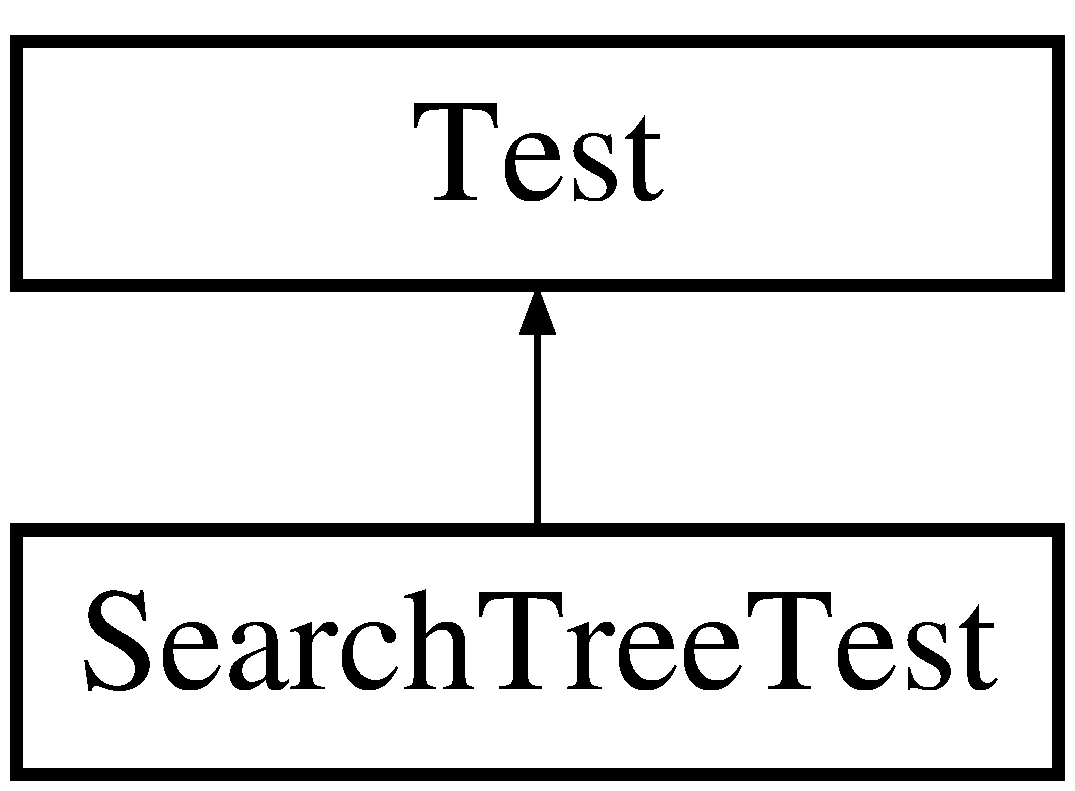
\includegraphics[height=2.000000cm]{class_search_tree_test}
\end{center}
\end{figure}
\subsection*{Public Types}
\begin{DoxyCompactItemize}
\item 
typedef \hyperlink{struct_introdunction_to_algorithm_1_1_tree_algorithm_1_1_binary_tree_node}{Binary\+Tree\+Node}$<$ int $>$ \hyperlink{class_search_tree_test_a921d5813f947eb9b70417b69722bc050}{Node}
\end{DoxyCompactItemize}
\subsection*{Protected Member Functions}
\begin{DoxyCompactItemize}
\item 
\hyperlink{class_search_tree_test_a8499bee6e18b14298bb210e067d04e99}{Search\+Tree\+Test} ()
\item 
void \hyperlink{class_search_tree_test_a90a211d1322c06e96bee25849525c77f}{Set\+Up} ()
\begin{DoxyCompactList}\small\item\em Set\+Up\+:在每一个测试开始之前执行 \end{DoxyCompactList}\item 
void \hyperlink{class_search_tree_test_a2fff7db7a798909e087a66ce890f4f49}{Tear\+Down} ()
\begin{DoxyCompactList}\small\item\em Tear\+Down\+:在每一个测试结束之后执行 \end{DoxyCompactList}\end{DoxyCompactItemize}
\subsection*{Protected Attributes}
\begin{DoxyCompactItemize}
\item 
\hyperlink{class_introdunction_to_algorithm_1_1_tree_algorithm_1_1_search_tree}{Search\+Tree}$<$ \hyperlink{class_search_tree_test_a921d5813f947eb9b70417b69722bc050}{Node} $>$ \hyperlink{class_search_tree_test_a08832932ab11e000dcd1ba60da8bad5f}{\+\_\+empty\+\_\+tree}
\item 
\hyperlink{class_introdunction_to_algorithm_1_1_tree_algorithm_1_1_search_tree}{Search\+Tree}$<$ \hyperlink{class_search_tree_test_a921d5813f947eb9b70417b69722bc050}{Node} $>$ \hyperlink{class_search_tree_test_a9982df0c932b171ff29dfe7abcebdc05}{\+\_\+normal\+\_\+tree}
\end{DoxyCompactItemize}


\subsection{Detailed Description}
\hyperlink{class_search_tree_test}{Search\+Tree\+Test}\+:测试类,用于为测试提供基础数据 

{\ttfamily \hyperlink{class_search_tree_test}{Search\+Tree\+Test}}是 {\ttfamily \+::testing\+::\+Test} 的子类。它主要用于为每一个{\ttfamily T\+E\+S\+T\+\_\+\+F}准备测试环境 

Definition at line 24 of file searchtree\+\_\+test.\+h.



\subsection{Member Typedef Documentation}
\hypertarget{class_search_tree_test_a921d5813f947eb9b70417b69722bc050}{}\index{Search\+Tree\+Test@{Search\+Tree\+Test}!Node@{Node}}
\index{Node@{Node}!Search\+Tree\+Test@{Search\+Tree\+Test}}
\subsubsection[{Node}]{\setlength{\rightskip}{0pt plus 5cm}typedef {\bf Binary\+Tree\+Node}$<$int$>$ {\bf Search\+Tree\+Test\+::\+Node}}\label{class_search_tree_test_a921d5813f947eb9b70417b69722bc050}


Definition at line 27 of file searchtree\+\_\+test.\+h.



\subsection{Constructor \& Destructor Documentation}
\hypertarget{class_search_tree_test_a8499bee6e18b14298bb210e067d04e99}{}\index{Search\+Tree\+Test@{Search\+Tree\+Test}!Search\+Tree\+Test@{Search\+Tree\+Test}}
\index{Search\+Tree\+Test@{Search\+Tree\+Test}!Search\+Tree\+Test@{Search\+Tree\+Test}}
\subsubsection[{Search\+Tree\+Test()}]{\setlength{\rightskip}{0pt plus 5cm}Search\+Tree\+Test\+::\+Search\+Tree\+Test (
\begin{DoxyParamCaption}
{}
\end{DoxyParamCaption}
)\hspace{0.3cm}{\ttfamily [inline]}, {\ttfamily [protected]}}\label{class_search_tree_test_a8499bee6e18b14298bb210e067d04e99}


Definition at line 29 of file searchtree\+\_\+test.\+h.



\subsection{Member Function Documentation}
\hypertarget{class_search_tree_test_a90a211d1322c06e96bee25849525c77f}{}\index{Search\+Tree\+Test@{Search\+Tree\+Test}!Set\+Up@{Set\+Up}}
\index{Set\+Up@{Set\+Up}!Search\+Tree\+Test@{Search\+Tree\+Test}}
\subsubsection[{Set\+Up()}]{\setlength{\rightskip}{0pt plus 5cm}void Search\+Tree\+Test\+::\+Set\+Up (
\begin{DoxyParamCaption}
{}
\end{DoxyParamCaption}
)\hspace{0.3cm}{\ttfamily [inline]}, {\ttfamily [protected]}}\label{class_search_tree_test_a90a211d1322c06e96bee25849525c77f}


Set\+Up\+:在每一个测试开始之前执行 

{\ttfamily Set\+Up}是 {\ttfamily \+::testing\+::\+Test} 的的虚函数。它主要用于为每一个测试提供测试环境 

Definition at line 36 of file searchtree\+\_\+test.\+h.

\hypertarget{class_search_tree_test_a2fff7db7a798909e087a66ce890f4f49}{}\index{Search\+Tree\+Test@{Search\+Tree\+Test}!Tear\+Down@{Tear\+Down}}
\index{Tear\+Down@{Tear\+Down}!Search\+Tree\+Test@{Search\+Tree\+Test}}
\subsubsection[{Tear\+Down()}]{\setlength{\rightskip}{0pt plus 5cm}void Search\+Tree\+Test\+::\+Tear\+Down (
\begin{DoxyParamCaption}
{}
\end{DoxyParamCaption}
)\hspace{0.3cm}{\ttfamily [inline]}, {\ttfamily [protected]}}\label{class_search_tree_test_a2fff7db7a798909e087a66ce890f4f49}


Tear\+Down\+:在每一个测试结束之后执行 

{\ttfamily Tear\+Down}是 {\ttfamily \+::testing\+::\+Test} 的的虚函数。它主要用于为每个测试销毁测试环境 

Definition at line 76 of file searchtree\+\_\+test.\+h.



\subsection{Member Data Documentation}
\hypertarget{class_search_tree_test_a08832932ab11e000dcd1ba60da8bad5f}{}\index{Search\+Tree\+Test@{Search\+Tree\+Test}!\+\_\+empty\+\_\+tree@{\+\_\+empty\+\_\+tree}}
\index{\+\_\+empty\+\_\+tree@{\+\_\+empty\+\_\+tree}!Search\+Tree\+Test@{Search\+Tree\+Test}}
\subsubsection[{\+\_\+empty\+\_\+tree}]{\setlength{\rightskip}{0pt plus 5cm}{\bf Search\+Tree}$<${\bf Node}$>$ Search\+Tree\+Test\+::\+\_\+empty\+\_\+tree\hspace{0.3cm}{\ttfamily [protected]}}\label{class_search_tree_test_a08832932ab11e000dcd1ba60da8bad5f}
一个空的树 

Definition at line 78 of file searchtree\+\_\+test.\+h.

\hypertarget{class_search_tree_test_a9982df0c932b171ff29dfe7abcebdc05}{}\index{Search\+Tree\+Test@{Search\+Tree\+Test}!\+\_\+normal\+\_\+tree@{\+\_\+normal\+\_\+tree}}
\index{\+\_\+normal\+\_\+tree@{\+\_\+normal\+\_\+tree}!Search\+Tree\+Test@{Search\+Tree\+Test}}
\subsubsection[{\+\_\+normal\+\_\+tree}]{\setlength{\rightskip}{0pt plus 5cm}{\bf Search\+Tree}$<${\bf Node}$>$ Search\+Tree\+Test\+::\+\_\+normal\+\_\+tree\hspace{0.3cm}{\ttfamily [protected]}}\label{class_search_tree_test_a9982df0c932b171ff29dfe7abcebdc05}
一个非空的数 

Definition at line 79 of file searchtree\+\_\+test.\+h.



The documentation for this class was generated from the following file\+:\begin{DoxyCompactItemize}
\item 
src/tree\+\_\+algorithms/searchtree/\hyperlink{searchtree__test_8h}{searchtree\+\_\+test.\+h}\end{DoxyCompactItemize}

\hypertarget{class_introdunction_to_algorithm_1_1_sort_algorithm_1_1_sort___heap}{}\section{Introdunction\+To\+Algorithm\+:\+:Sort\+Algorithm\+:\+:Sort\+\_\+\+Heap$<$ Iterator, Compare $>$ Class Template Reference}
\label{class_introdunction_to_algorithm_1_1_sort_algorithm_1_1_sort___heap}\index{Introdunction\+To\+Algorithm\+::\+Sort\+Algorithm\+::\+Sort\+\_\+\+Heap$<$ Iterator, Compare $>$@{Introdunction\+To\+Algorithm\+::\+Sort\+Algorithm\+::\+Sort\+\_\+\+Heap$<$ Iterator, Compare $>$}}


Sort\+\_\+\+Heap:用于堆排序的堆,算法导论第6章  




{\ttfamily \#include $<$heapsort.\+h$>$}

\subsection*{Public Types}
\begin{DoxyCompactItemize}
\item 
typedef std\+::iterator\+\_\+traits$<$ Iterator $>$\+::value\+\_\+type \hyperlink{class_introdunction_to_algorithm_1_1_sort_algorithm_1_1_sort___heap_a919579152d685b356d4776fc8d2eeb90}{T}
\end{DoxyCompactItemize}
\subsection*{Public Member Functions}
\begin{DoxyCompactItemize}
\item 
void \hyperlink{class_introdunction_to_algorithm_1_1_sort_algorithm_1_1_sort___heap_a3c6f55939475aac8e7651248230e1730}{operator()} (const Iterator from, std\+::size\+\_\+t size, Compare compare=Compare())
\begin{DoxyCompactList}\small\item\em operator() \end{DoxyCompactList}\end{DoxyCompactItemize}
\subsection*{Private Member Functions}
\begin{DoxyCompactItemize}
\item 
void \hyperlink{class_introdunction_to_algorithm_1_1_sort_algorithm_1_1_sort___heap_ab8b98e11afa86430214c6998c48b21d1}{\+\_\+setup\+Heap} (Compare compare=Compare())
\begin{DoxyCompactList}\small\item\em \+\_\+setup\+Heap\+:建堆 \end{DoxyCompactList}\item 
void \hyperlink{class_introdunction_to_algorithm_1_1_sort_algorithm_1_1_sort___heap_a12f57e7bb47939f0f4f0994ee81d4b9e}{\+\_\+heapify} (std\+::size\+\_\+t element\+Index, Compare compare=Compare())
\begin{DoxyCompactList}\small\item\em \+\_\+heapify:维持堆性质 \end{DoxyCompactList}\item 
std\+::size\+\_\+t \hyperlink{class_introdunction_to_algorithm_1_1_sort_algorithm_1_1_sort___heap_a2607ad45b37fb4dde8e2c94e50cd19da}{\+\_\+parent\+Index} (std\+::size\+\_\+t element\+Index, bool \&valid)
\begin{DoxyCompactList}\small\item\em \+\_\+parent\+Index\+:返回一个节点的父节点位置 \end{DoxyCompactList}\item 
std\+::size\+\_\+t \hyperlink{class_introdunction_to_algorithm_1_1_sort_algorithm_1_1_sort___heap_a0ba289760dd936944dc2629511c73f27}{\+\_\+lchild\+Index} (std\+::size\+\_\+t element\+Index, bool \&valid)
\begin{DoxyCompactList}\small\item\em \+\_\+lchild\+Index\+:返回一个节点的左子节点位置 \end{DoxyCompactList}\item 
std\+::size\+\_\+t \hyperlink{class_introdunction_to_algorithm_1_1_sort_algorithm_1_1_sort___heap_abb4d45e22fc4fc5ec297214f28605209}{\+\_\+rchild\+Index} (std\+::size\+\_\+t element\+Index, bool \&valid)
\begin{DoxyCompactList}\small\item\em \+\_\+rchild\+Index\+:返回一个节点的右子节点位置 \end{DoxyCompactList}\end{DoxyCompactItemize}
\subsection*{Private Attributes}
\begin{DoxyCompactItemize}
\item 
Iterator \hyperlink{class_introdunction_to_algorithm_1_1_sort_algorithm_1_1_sort___heap_a7f6c20382257308edd2c0049ec46ad66}{\+\_\+from}
\item 
std\+::size\+\_\+t \hyperlink{class_introdunction_to_algorithm_1_1_sort_algorithm_1_1_sort___heap_a3cbf6e8a1972cc62bce0b50226024a52}{\+\_\+size}
\end{DoxyCompactItemize}


\subsection{Detailed Description}
\subsubsection*{template$<$typename Iterator, typename Compare = std\+::less$<$typename std\+::iterator\+\_\+traits$<$\+Iterator$>$\+::value\+\_\+type$>$$>$class Introdunction\+To\+Algorithm\+::\+Sort\+Algorithm\+::\+Sort\+\_\+\+Heap$<$ Iterator, Compare $>$}

Sort\+\_\+\+Heap:用于堆排序的堆,算法导论第6章 


\begin{DoxyItemize}
\item 堆排序思想:假设对数组\+A\mbox{[}p...r\mbox{]}排序:首先将数组构建成一个最小堆(或者最大堆)。然后第一个元素就是堆中最小的元素。 将第一个元素与最后一个元素交换,同时堆的规模缩减1,再将堆维持最小堆性质。不断循环最后得到一个排序好的数组 $\ast$
\item 时间复杂度 O(nlogn)
\item 原地排序
\end{DoxyItemize}

堆排序有两个重要操作:


\begin{DoxyItemize}
\item heapify(index)操作:维持以index为根节点的子堆的性质。它比较index与其左右子节点的值,选取其最小的那个提升到index节点上。同时递归向下。具体见\+\_\+heapify()方法说明
\item setup\+Heap()操作: 建堆操作。它从堆的最低层向上层反复调用heapify操作进行建堆。 
\end{DoxyItemize}

Definition at line 22 of file heapsort.\+h.



\subsection{Member Typedef Documentation}
\hypertarget{class_introdunction_to_algorithm_1_1_sort_algorithm_1_1_sort___heap_a919579152d685b356d4776fc8d2eeb90}{}\index{Introdunction\+To\+Algorithm\+::\+Sort\+Algorithm\+::\+Sort\+\_\+\+Heap@{Introdunction\+To\+Algorithm\+::\+Sort\+Algorithm\+::\+Sort\+\_\+\+Heap}!T@{T}}
\index{T@{T}!Introdunction\+To\+Algorithm\+::\+Sort\+Algorithm\+::\+Sort\+\_\+\+Heap@{Introdunction\+To\+Algorithm\+::\+Sort\+Algorithm\+::\+Sort\+\_\+\+Heap}}
\subsubsection[{T}]{\setlength{\rightskip}{0pt plus 5cm}template$<$typename Iterator, typename Compare = std\+::less$<$typename std\+::iterator\+\_\+traits$<$\+Iterator$>$\+::value\+\_\+type$>$$>$ typedef std\+::iterator\+\_\+traits$<$Iterator$>$\+::value\+\_\+type {\bf Introdunction\+To\+Algorithm\+::\+Sort\+Algorithm\+::\+Sort\+\_\+\+Heap}$<$ Iterator, Compare $>$\+::{\bf T}}\label{class_introdunction_to_algorithm_1_1_sort_algorithm_1_1_sort___heap_a919579152d685b356d4776fc8d2eeb90}
迭代器指向对象的值类型 

Definition at line 25 of file heapsort.\+h.



\subsection{Member Function Documentation}
\hypertarget{class_introdunction_to_algorithm_1_1_sort_algorithm_1_1_sort___heap_a12f57e7bb47939f0f4f0994ee81d4b9e}{}\index{Introdunction\+To\+Algorithm\+::\+Sort\+Algorithm\+::\+Sort\+\_\+\+Heap@{Introdunction\+To\+Algorithm\+::\+Sort\+Algorithm\+::\+Sort\+\_\+\+Heap}!\+\_\+heapify@{\+\_\+heapify}}
\index{\+\_\+heapify@{\+\_\+heapify}!Introdunction\+To\+Algorithm\+::\+Sort\+Algorithm\+::\+Sort\+\_\+\+Heap@{Introdunction\+To\+Algorithm\+::\+Sort\+Algorithm\+::\+Sort\+\_\+\+Heap}}
\subsubsection[{\+\_\+heapify(std\+::size\+\_\+t element\+Index, Compare compare=\+Compare())}]{\setlength{\rightskip}{0pt plus 5cm}template$<$typename Iterator, typename Compare = std\+::less$<$typename std\+::iterator\+\_\+traits$<$\+Iterator$>$\+::value\+\_\+type$>$$>$ void {\bf Introdunction\+To\+Algorithm\+::\+Sort\+Algorithm\+::\+Sort\+\_\+\+Heap}$<$ Iterator, Compare $>$\+::\+\_\+heapify (
\begin{DoxyParamCaption}
\item[{std\+::size\+\_\+t}]{element\+Index, }
\item[{Compare}]{compare = {\ttfamily Compare()}}
\end{DoxyParamCaption}
)\hspace{0.3cm}{\ttfamily [inline]}, {\ttfamily [private]}}\label{class_introdunction_to_algorithm_1_1_sort_algorithm_1_1_sort___heap_a12f57e7bb47939f0f4f0994ee81d4b9e}


\+\_\+heapify:维持堆性质 


\begin{DoxyParams}{Parameters}
{\em element\+Index} & \+: 要维持以该节点为根节点的子堆的堆性质 \\
\hline
{\em compare} & 一个可调用对象,可用于比较两个对象的小于比较,默认为std\+::less$<$\+T$>$ \\
\hline
\end{DoxyParams}
\begin{DoxyReturn}{Returns}
void
\end{DoxyReturn}
首先调用比较该节点与左右子节点的最小值。如果最小值为它本身,则维持了性质,返回;如果最小值不是它本身,那么必然为左、右子节点之一。 将该最小节点(假设为左子节点)交换到根节点,然后以左子节点递归调用heapify操作


\begin{DoxyItemize}
\item 时间复杂度 O(n)
\item 原地操作 
\end{DoxyItemize}

Definition at line 84 of file heapsort.\+h.

\hypertarget{class_introdunction_to_algorithm_1_1_sort_algorithm_1_1_sort___heap_a0ba289760dd936944dc2629511c73f27}{}\index{Introdunction\+To\+Algorithm\+::\+Sort\+Algorithm\+::\+Sort\+\_\+\+Heap@{Introdunction\+To\+Algorithm\+::\+Sort\+Algorithm\+::\+Sort\+\_\+\+Heap}!\+\_\+lchild\+Index@{\+\_\+lchild\+Index}}
\index{\+\_\+lchild\+Index@{\+\_\+lchild\+Index}!Introdunction\+To\+Algorithm\+::\+Sort\+Algorithm\+::\+Sort\+\_\+\+Heap@{Introdunction\+To\+Algorithm\+::\+Sort\+Algorithm\+::\+Sort\+\_\+\+Heap}}
\subsubsection[{\+\_\+lchild\+Index(std\+::size\+\_\+t element\+Index, bool \&valid)}]{\setlength{\rightskip}{0pt plus 5cm}template$<$typename Iterator, typename Compare = std\+::less$<$typename std\+::iterator\+\_\+traits$<$\+Iterator$>$\+::value\+\_\+type$>$$>$ std\+::size\+\_\+t {\bf Introdunction\+To\+Algorithm\+::\+Sort\+Algorithm\+::\+Sort\+\_\+\+Heap}$<$ Iterator, Compare $>$\+::\+\_\+lchild\+Index (
\begin{DoxyParamCaption}
\item[{std\+::size\+\_\+t}]{element\+Index, }
\item[{bool \&}]{valid}
\end{DoxyParamCaption}
)\hspace{0.3cm}{\ttfamily [inline]}, {\ttfamily [private]}}\label{class_introdunction_to_algorithm_1_1_sort_algorithm_1_1_sort___heap_a0ba289760dd936944dc2629511c73f27}


\+\_\+lchild\+Index\+:返回一个节点的左子节点位置 


\begin{DoxyParams}{Parameters}
{\em element\+Index} & \+: 节点位置 \\
\hline
{\em valid} & 一个bool\&值,用于返回,指示子节点是否有效 \\
\hline
\end{DoxyParams}
\begin{DoxyReturn}{Returns}
左子节点位置(std\+::size\+\_\+t)
\end{DoxyReturn}
根据最小堆的性质,一个节点element\+Index的左子节点是它的位置(element\+Index/2)+1


\begin{DoxyItemize}
\item 当最小堆大小为0、1时,它没有左子节点,左子节点无效
\item 当左子节点超过堆大小时,它无效 
\end{DoxyItemize}

Definition at line 144 of file heapsort.\+h.

\hypertarget{class_introdunction_to_algorithm_1_1_sort_algorithm_1_1_sort___heap_a2607ad45b37fb4dde8e2c94e50cd19da}{}\index{Introdunction\+To\+Algorithm\+::\+Sort\+Algorithm\+::\+Sort\+\_\+\+Heap@{Introdunction\+To\+Algorithm\+::\+Sort\+Algorithm\+::\+Sort\+\_\+\+Heap}!\+\_\+parent\+Index@{\+\_\+parent\+Index}}
\index{\+\_\+parent\+Index@{\+\_\+parent\+Index}!Introdunction\+To\+Algorithm\+::\+Sort\+Algorithm\+::\+Sort\+\_\+\+Heap@{Introdunction\+To\+Algorithm\+::\+Sort\+Algorithm\+::\+Sort\+\_\+\+Heap}}
\subsubsection[{\+\_\+parent\+Index(std\+::size\+\_\+t element\+Index, bool \&valid)}]{\setlength{\rightskip}{0pt plus 5cm}template$<$typename Iterator, typename Compare = std\+::less$<$typename std\+::iterator\+\_\+traits$<$\+Iterator$>$\+::value\+\_\+type$>$$>$ std\+::size\+\_\+t {\bf Introdunction\+To\+Algorithm\+::\+Sort\+Algorithm\+::\+Sort\+\_\+\+Heap}$<$ Iterator, Compare $>$\+::\+\_\+parent\+Index (
\begin{DoxyParamCaption}
\item[{std\+::size\+\_\+t}]{element\+Index, }
\item[{bool \&}]{valid}
\end{DoxyParamCaption}
)\hspace{0.3cm}{\ttfamily [inline]}, {\ttfamily [private]}}\label{class_introdunction_to_algorithm_1_1_sort_algorithm_1_1_sort___heap_a2607ad45b37fb4dde8e2c94e50cd19da}


\+\_\+parent\+Index\+:返回一个节点的父节点位置 


\begin{DoxyParams}{Parameters}
{\em element\+Index} & \+: 子节点位置 \\
\hline
{\em valid} & 一个bool\&值,用于返回,指示父节点是否有效 \\
\hline
\end{DoxyParams}
\begin{DoxyReturn}{Returns}
父节点位置(std\+::size\+\_\+t)
\end{DoxyReturn}
根据最小堆的性质,一个子节点element\+Index的父节点是它的位置(element\+Index-\/1)/2。


\begin{DoxyItemize}
\item 超出堆大小的节点,其父节点无效 
\end{DoxyItemize}

Definition at line 121 of file heapsort.\+h.

\hypertarget{class_introdunction_to_algorithm_1_1_sort_algorithm_1_1_sort___heap_abb4d45e22fc4fc5ec297214f28605209}{}\index{Introdunction\+To\+Algorithm\+::\+Sort\+Algorithm\+::\+Sort\+\_\+\+Heap@{Introdunction\+To\+Algorithm\+::\+Sort\+Algorithm\+::\+Sort\+\_\+\+Heap}!\+\_\+rchild\+Index@{\+\_\+rchild\+Index}}
\index{\+\_\+rchild\+Index@{\+\_\+rchild\+Index}!Introdunction\+To\+Algorithm\+::\+Sort\+Algorithm\+::\+Sort\+\_\+\+Heap@{Introdunction\+To\+Algorithm\+::\+Sort\+Algorithm\+::\+Sort\+\_\+\+Heap}}
\subsubsection[{\+\_\+rchild\+Index(std\+::size\+\_\+t element\+Index, bool \&valid)}]{\setlength{\rightskip}{0pt plus 5cm}template$<$typename Iterator, typename Compare = std\+::less$<$typename std\+::iterator\+\_\+traits$<$\+Iterator$>$\+::value\+\_\+type$>$$>$ std\+::size\+\_\+t {\bf Introdunction\+To\+Algorithm\+::\+Sort\+Algorithm\+::\+Sort\+\_\+\+Heap}$<$ Iterator, Compare $>$\+::\+\_\+rchild\+Index (
\begin{DoxyParamCaption}
\item[{std\+::size\+\_\+t}]{element\+Index, }
\item[{bool \&}]{valid}
\end{DoxyParamCaption}
)\hspace{0.3cm}{\ttfamily [inline]}, {\ttfamily [private]}}\label{class_introdunction_to_algorithm_1_1_sort_algorithm_1_1_sort___heap_abb4d45e22fc4fc5ec297214f28605209}


\+\_\+rchild\+Index\+:返回一个节点的右子节点位置 


\begin{DoxyParams}{Parameters}
{\em element\+Index} & \+: 节点位置 \\
\hline
{\em valid} & 一个bool\&值,用于返回,指示子节点是否有效 \\
\hline
\end{DoxyParams}
\begin{DoxyReturn}{Returns}
右子节点位置(std\+::size\+\_\+t)
\end{DoxyReturn}
根据最小堆的性质,一个节点element\+Index的右子节点是它的位置(element\+Index/2)+2


\begin{DoxyItemize}
\item 当最小堆大小为0、、1、2时,它没有右子节点,右子节点无效
\item 当右子节点超过堆大小时,它无效 
\end{DoxyItemize}

Definition at line 172 of file heapsort.\+h.

\hypertarget{class_introdunction_to_algorithm_1_1_sort_algorithm_1_1_sort___heap_ab8b98e11afa86430214c6998c48b21d1}{}\index{Introdunction\+To\+Algorithm\+::\+Sort\+Algorithm\+::\+Sort\+\_\+\+Heap@{Introdunction\+To\+Algorithm\+::\+Sort\+Algorithm\+::\+Sort\+\_\+\+Heap}!\+\_\+setup\+Heap@{\+\_\+setup\+Heap}}
\index{\+\_\+setup\+Heap@{\+\_\+setup\+Heap}!Introdunction\+To\+Algorithm\+::\+Sort\+Algorithm\+::\+Sort\+\_\+\+Heap@{Introdunction\+To\+Algorithm\+::\+Sort\+Algorithm\+::\+Sort\+\_\+\+Heap}}
\subsubsection[{\+\_\+setup\+Heap(\+Compare compare=\+Compare())}]{\setlength{\rightskip}{0pt plus 5cm}template$<$typename Iterator, typename Compare = std\+::less$<$typename std\+::iterator\+\_\+traits$<$\+Iterator$>$\+::value\+\_\+type$>$$>$ void {\bf Introdunction\+To\+Algorithm\+::\+Sort\+Algorithm\+::\+Sort\+\_\+\+Heap}$<$ Iterator, Compare $>$\+::\+\_\+setup\+Heap (
\begin{DoxyParamCaption}
\item[{Compare}]{compare = {\ttfamily Compare()}}
\end{DoxyParamCaption}
)\hspace{0.3cm}{\ttfamily [inline]}, {\ttfamily [private]}}\label{class_introdunction_to_algorithm_1_1_sort_algorithm_1_1_sort___heap_ab8b98e11afa86430214c6998c48b21d1}


\+\_\+setup\+Heap\+:建堆 


\begin{DoxyParams}{Parameters}
{\em compare} & 一个可调用对象,可用于比较两个对象的小于比较,默认为std\+::less$<$\+T$>$ \\
\hline
\end{DoxyParams}
\begin{DoxyReturn}{Returns}
void
\end{DoxyReturn}
从后一半的元素开始依次向前调用heapify操作(根据最小堆性质,除了最底层它是完全充满的)


\begin{DoxyItemize}
\item 时间复杂度 O(nlogn)
\item 原地操作 
\end{DoxyItemize}

Definition at line 61 of file heapsort.\+h.

\hypertarget{class_introdunction_to_algorithm_1_1_sort_algorithm_1_1_sort___heap_a3c6f55939475aac8e7651248230e1730}{}\index{Introdunction\+To\+Algorithm\+::\+Sort\+Algorithm\+::\+Sort\+\_\+\+Heap@{Introdunction\+To\+Algorithm\+::\+Sort\+Algorithm\+::\+Sort\+\_\+\+Heap}!operator()@{operator()}}
\index{operator()@{operator()}!Introdunction\+To\+Algorithm\+::\+Sort\+Algorithm\+::\+Sort\+\_\+\+Heap@{Introdunction\+To\+Algorithm\+::\+Sort\+Algorithm\+::\+Sort\+\_\+\+Heap}}
\subsubsection[{operator()(const Iterator from, std\+::size\+\_\+t size, Compare compare=\+Compare())}]{\setlength{\rightskip}{0pt plus 5cm}template$<$typename Iterator, typename Compare = std\+::less$<$typename std\+::iterator\+\_\+traits$<$\+Iterator$>$\+::value\+\_\+type$>$$>$ void {\bf Introdunction\+To\+Algorithm\+::\+Sort\+Algorithm\+::\+Sort\+\_\+\+Heap}$<$ Iterator, Compare $>$\+::operator() (
\begin{DoxyParamCaption}
\item[{const Iterator}]{from, }
\item[{std\+::size\+\_\+t}]{size, }
\item[{Compare}]{compare = {\ttfamily Compare()}}
\end{DoxyParamCaption}
)\hspace{0.3cm}{\ttfamily [inline]}}\label{class_introdunction_to_algorithm_1_1_sort_algorithm_1_1_sort___heap_a3c6f55939475aac8e7651248230e1730}


operator() 


\begin{DoxyParams}{Parameters}
{\em from} & \+: 待排序序列的起始迭代器(也可以是指向数组中某元素的指针) \\
\hline
{\em size} & 待排序序列的长度 \\
\hline
{\em compare} & 一个可调用对象,可用于比较两个对象的小于比较,默认为std\+::less$<$\+T$>$ \\
\hline
\end{DoxyParams}
\begin{DoxyReturn}{Returns}
void
\end{DoxyReturn}
首先调用 \hyperlink{class_introdunction_to_algorithm_1_1_sort_algorithm_1_1_sort___heap_ab8b98e11afa86430214c6998c48b21d1}{\+\_\+setup\+Heap()}建堆。然后再反复抽取最小值到堆尾部,然后维持堆的性质。


\begin{DoxyItemize}
\item 时间复杂度 O(nlogn)
\item 原地排序 
\end{DoxyItemize}

Definition at line 38 of file heapsort.\+h.



\subsection{Member Data Documentation}
\hypertarget{class_introdunction_to_algorithm_1_1_sort_algorithm_1_1_sort___heap_a7f6c20382257308edd2c0049ec46ad66}{}\index{Introdunction\+To\+Algorithm\+::\+Sort\+Algorithm\+::\+Sort\+\_\+\+Heap@{Introdunction\+To\+Algorithm\+::\+Sort\+Algorithm\+::\+Sort\+\_\+\+Heap}!\+\_\+from@{\+\_\+from}}
\index{\+\_\+from@{\+\_\+from}!Introdunction\+To\+Algorithm\+::\+Sort\+Algorithm\+::\+Sort\+\_\+\+Heap@{Introdunction\+To\+Algorithm\+::\+Sort\+Algorithm\+::\+Sort\+\_\+\+Heap}}
\subsubsection[{\+\_\+from}]{\setlength{\rightskip}{0pt plus 5cm}template$<$typename Iterator, typename Compare = std\+::less$<$typename std\+::iterator\+\_\+traits$<$\+Iterator$>$\+::value\+\_\+type$>$$>$ Iterator {\bf Introdunction\+To\+Algorithm\+::\+Sort\+Algorithm\+::\+Sort\+\_\+\+Heap}$<$ Iterator, Compare $>$\+::\+\_\+from\hspace{0.3cm}{\ttfamily [private]}}\label{class_introdunction_to_algorithm_1_1_sort_algorithm_1_1_sort___heap_a7f6c20382257308edd2c0049ec46ad66}
堆根节点位置 

Definition at line 188 of file heapsort.\+h.

\hypertarget{class_introdunction_to_algorithm_1_1_sort_algorithm_1_1_sort___heap_a3cbf6e8a1972cc62bce0b50226024a52}{}\index{Introdunction\+To\+Algorithm\+::\+Sort\+Algorithm\+::\+Sort\+\_\+\+Heap@{Introdunction\+To\+Algorithm\+::\+Sort\+Algorithm\+::\+Sort\+\_\+\+Heap}!\+\_\+size@{\+\_\+size}}
\index{\+\_\+size@{\+\_\+size}!Introdunction\+To\+Algorithm\+::\+Sort\+Algorithm\+::\+Sort\+\_\+\+Heap@{Introdunction\+To\+Algorithm\+::\+Sort\+Algorithm\+::\+Sort\+\_\+\+Heap}}
\subsubsection[{\+\_\+size}]{\setlength{\rightskip}{0pt plus 5cm}template$<$typename Iterator, typename Compare = std\+::less$<$typename std\+::iterator\+\_\+traits$<$\+Iterator$>$\+::value\+\_\+type$>$$>$ std\+::size\+\_\+t {\bf Introdunction\+To\+Algorithm\+::\+Sort\+Algorithm\+::\+Sort\+\_\+\+Heap}$<$ Iterator, Compare $>$\+::\+\_\+size\hspace{0.3cm}{\ttfamily [private]}}\label{class_introdunction_to_algorithm_1_1_sort_algorithm_1_1_sort___heap_a3cbf6e8a1972cc62bce0b50226024a52}
堆大小 

Definition at line 189 of file heapsort.\+h.



The documentation for this class was generated from the following file\+:\begin{DoxyCompactItemize}
\item 
src/sort\+\_\+algorithms/heap\+\_\+sort/\hyperlink{heapsort_8h}{heapsort.\+h}\end{DoxyCompactItemize}

\chapter{File Documentation}
\hypertarget{algorithms_8h}{}\section{src/algorithms.h File Reference}
\label{algorithms_8h}\index{src/algorithms.\+h@{src/algorithms.\+h}}
{\ttfamily \#include $<$string$>$}\\*
{\ttfamily \#include $<$iostream$>$}\\*
\subsection*{Namespaces}
\begin{DoxyCompactItemize}
\item 
 \hyperlink{namespace_introdunction_to_algorithm}{Introdunction\+To\+Algorithm}
\begin{DoxyCompactList}\small\item\em Namespace of \hyperlink{namespace_introdunction_to_algorithm}{Introdunction\+To\+Algorithm}. \end{DoxyCompactList}\item 
 \hyperlink{namespace_introdunction_to_algorithm_1_1_sort_algorithm}{Introdunction\+To\+Algorithm\+::\+Sort\+Algorithm}
\begin{DoxyCompactList}\small\item\em Namespace of \hyperlink{namespace_introdunction_to_algorithm_1_1_sort_algorithm}{Sort\+Algorithm}. \end{DoxyCompactList}\item 
 \hyperlink{namespace_introdunction_to_algorithm_1_1_select_algorithm}{Introdunction\+To\+Algorithm\+::\+Select\+Algorithm}
\begin{DoxyCompactList}\small\item\em Namespace of \hyperlink{namespace_introdunction_to_algorithm_1_1_select_algorithm}{Select\+Algorithm}. \end{DoxyCompactList}\end{DoxyCompactItemize}

\hypertarget{longest__common__subsequence_8h}{}\section{src/dynamic\+\_\+programmitn\+\_\+algorithms/longest\+\_\+common\+\_\+subsequence.h File Reference}
\label{longest__common__subsequence_8h}\index{src/dynamic\+\_\+programmitn\+\_\+algorithms/longest\+\_\+common\+\_\+subsequence.\+h@{src/dynamic\+\_\+programmitn\+\_\+algorithms/longest\+\_\+common\+\_\+subsequence.\+h}}
{\ttfamily \#include $<$type\+\_\+traits$>$}\\*
{\ttfamily \#include $<$vector$>$}\\*
{\ttfamily \#include $<$iostream$>$}\\*
\subsection*{Namespaces}
\begin{DoxyCompactItemize}
\item 
 \hyperlink{namespace_introdunction_to_algorithm}{Introdunction\+To\+Algorithm}
\begin{DoxyCompactList}\small\item\em Namespace of \hyperlink{namespace_introdunction_to_algorithm}{Introdunction\+To\+Algorithm}. \end{DoxyCompactList}\item 
 \hyperlink{namespace_introdunction_to_algorithm_1_1_dynamic_programming_algorithm}{Introdunction\+To\+Algorithm\+::\+Dynamic\+Programming\+Algorithm}
\begin{DoxyCompactList}\small\item\em Namespace of \hyperlink{namespace_introdunction_to_algorithm_1_1_dynamic_programming_algorithm}{Dynamic\+Programming\+Algorithm}. \end{DoxyCompactList}\end{DoxyCompactItemize}
\subsection*{Functions}
\begin{DoxyCompactItemize}
\item 
{\footnotesize template$<$typename Iterator , typename Out\+Iterator $>$ }\\std\+::size\+\_\+t \hyperlink{namespace_introdunction_to_algorithm_1_1_dynamic_programming_algorithm_a01cfb7cc6a668a29024f83a65481196b}{Introdunction\+To\+Algorithm\+::\+Dynamic\+Programming\+Algorithm\+::make\+\_\+\+L\+C\+S} (const Iterator begin, const Iterator end, const std\+::vector$<$ std\+::vector$<$ int $>$$>$ \&flag\+\_\+matrix, typename std\+::iterator\+\_\+traits$<$ Iterator $>$\+::difference\+\_\+type seq1\+\_\+index, typename std\+::iterator\+\_\+traits$<$ Iterator $>$\+::difference\+\_\+type seq2\+\_\+index, Out\+Iterator \&out\+\_\+begin)
\begin{DoxyCompactList}\small\item\em make\+\_\+\+L\+C\+S 最长公共子序列的子算法:已知标记矩阵,求最长公共子序列 \end{DoxyCompactList}\item 
{\footnotesize template$<$typename Iterator1 , typename Iterator2 , typename Out\+Iterator $>$ }\\std\+::size\+\_\+t \hyperlink{namespace_introdunction_to_algorithm_1_1_dynamic_programming_algorithm_a000f514133c72dd4c28127bc83e7bf02}{Introdunction\+To\+Algorithm\+::\+Dynamic\+Programming\+Algorithm\+::longest\+\_\+common\+\_\+subsequence} (const Iterator1 first\+\_\+begin, const Iterator1 first\+\_\+end, const Iterator2 second\+\_\+begin, const Iterator2 second\+\_\+end, Out\+Iterator out\+\_\+begin)
\begin{DoxyCompactList}\small\item\em longest\+\_\+common\+\_\+subsequence 算法导论第15章9.4 最长公共子序列 \end{DoxyCompactList}\end{DoxyCompactItemize}

\hypertarget{longest__common__subsequence__test_8h}{}\section{src/dynamic\+\_\+programmitn\+\_\+algorithms/longest\+\_\+common\+\_\+subsequence\+\_\+test.h File Reference}
\label{longest__common__subsequence__test_8h}\index{src/dynamic\+\_\+programmitn\+\_\+algorithms/longest\+\_\+common\+\_\+subsequence\+\_\+test.\+h@{src/dynamic\+\_\+programmitn\+\_\+algorithms/longest\+\_\+common\+\_\+subsequence\+\_\+test.\+h}}
{\ttfamily \#include \char`\"{}src/google\+\_\+test/gtest.\+h\char`\"{}}\\*
{\ttfamily \#include \char`\"{}src/dynamic\+\_\+programmitn\+\_\+algorithms/longest\+\_\+common\+\_\+subsequence.\+h\char`\"{}}\\*
\subsection*{Functions}
\begin{DoxyCompactItemize}
\item 
\hyperlink{longest__common__subsequence__test_8h_af6d25933a23afb7fa7f99323fe0808ea}{T\+E\+S\+T} (test\+\_\+longest\+\_\+common\+\_\+subsequence, test1)
\begin{DoxyCompactList}\small\item\em longest\+\_\+common\+\_\+subsequence\+\_\+test:测试最长公共子数组 \end{DoxyCompactList}\end{DoxyCompactItemize}


\subsection{Function Documentation}
\hypertarget{longest__common__subsequence__test_8h_af6d25933a23afb7fa7f99323fe0808ea}{}\index{longest\+\_\+common\+\_\+subsequence\+\_\+test.\+h@{longest\+\_\+common\+\_\+subsequence\+\_\+test.\+h}!T\+E\+S\+T@{T\+E\+S\+T}}
\index{T\+E\+S\+T@{T\+E\+S\+T}!longest\+\_\+common\+\_\+subsequence\+\_\+test.\+h@{longest\+\_\+common\+\_\+subsequence\+\_\+test.\+h}}
\subsubsection[{T\+E\+S\+T(test\+\_\+longest\+\_\+common\+\_\+subsequence, test1)}]{\setlength{\rightskip}{0pt plus 5cm}T\+E\+S\+T (
\begin{DoxyParamCaption}
\item[{test\+\_\+longest\+\_\+common\+\_\+subsequence}]{, }
\item[{test1}]{}
\end{DoxyParamCaption}
)}\label{longest__common__subsequence__test_8h_af6d25933a23afb7fa7f99323fe0808ea}


longest\+\_\+common\+\_\+subsequence\+\_\+test:测试最长公共子数组 

三组数据: s1为空字符串s2为非空字符串、s1和s2为常规字符串且二者内容不等、s1和s2为常规字符串且二者内容相等 

Definition at line 12 of file longest\+\_\+common\+\_\+subsequence\+\_\+test.\+h.


\hypertarget{goodselect_8h}{}\section{src/select\+\_\+algorithms/good\+\_\+select/goodselect.h File Reference}
\label{goodselect_8h}\index{src/select\+\_\+algorithms/good\+\_\+select/goodselect.\+h@{src/select\+\_\+algorithms/good\+\_\+select/goodselect.\+h}}
{\ttfamily \#include $<$vector$>$}\\*
{\ttfamily \#include \char`\"{}src/sort\+\_\+algorithms/quick\+\_\+sort/quicksort.\+h\char`\"{}}\\*
\subsection*{Namespaces}
\begin{DoxyCompactItemize}
\item 
 \hyperlink{namespace_introdunction_to_algorithm}{Introdunction\+To\+Algorithm}
\begin{DoxyCompactList}\small\item\em Namespace of \hyperlink{namespace_introdunction_to_algorithm}{Introdunction\+To\+Algorithm}. \end{DoxyCompactList}\item 
 \hyperlink{namespace_introdunction_to_algorithm_1_1_select_algorithm}{Introdunction\+To\+Algorithm\+::\+Select\+Algorithm}
\begin{DoxyCompactList}\small\item\em Namespace of \hyperlink{namespace_introdunction_to_algorithm_1_1_select_algorithm}{Select\+Algorithm}. \end{DoxyCompactList}\end{DoxyCompactItemize}
\subsection*{Functions}
\begin{DoxyCompactItemize}
\item 
{\footnotesize template$<$typename Iterator , typename Compare  = std\+::less$<$typename std\+::iterator\+\_\+traits$<$\+Iterator$>$\+::value\+\_\+type$>$$>$ }\\std\+::iterator\+\_\+traits$<$ Iterator $>$\+::value\+\_\+type \hyperlink{namespace_introdunction_to_algorithm_1_1_select_algorithm_a1a12272ccfaf7b91916aed885085b86c}{Introdunction\+To\+Algorithm\+::\+Select\+Algorithm\+::good\+\_\+select} (const Iterator begin, const Iterator end, typename std\+::iterator\+\_\+traits$<$ Iterator $>$\+::difference\+\_\+type rank, Compare compare=Compare())
\begin{DoxyCompactList}\small\item\em good\+\_\+select: 算法导论第9章9.3 最坏时间为\+O(n)的顺序统计量选择算法 \end{DoxyCompactList}\end{DoxyCompactItemize}

\hypertarget{goodselect__test_8h}{}\section{src/select\+\_\+algorithms/good\+\_\+select/goodselect\+\_\+test.h File Reference}
\label{goodselect__test_8h}\index{src/select\+\_\+algorithms/good\+\_\+select/goodselect\+\_\+test.\+h@{src/select\+\_\+algorithms/good\+\_\+select/goodselect\+\_\+test.\+h}}
{\ttfamily \#include \char`\"{}src/google\+\_\+test/gtest.\+h\char`\"{}}\\*
{\ttfamily \#include \char`\"{}goodselect.\+h\char`\"{}}\\*
\subsection*{Functions}
\begin{DoxyCompactItemize}
\item 
\hyperlink{goodselect__test_8h_a8a288d2a03049b97c95b8643d48ea455}{T\+E\+S\+T} (test\+\_\+good\+\_\+select, test\+\_\+\+C\+\_\+array)
\begin{DoxyCompactList}\small\item\em good\+\_\+select\+\_\+test:测试\+C数组的顺序统计量 \end{DoxyCompactList}\end{DoxyCompactItemize}


\subsection{Function Documentation}
\hypertarget{goodselect__test_8h_a8a288d2a03049b97c95b8643d48ea455}{}\index{goodselect\+\_\+test.\+h@{goodselect\+\_\+test.\+h}!T\+E\+S\+T@{T\+E\+S\+T}}
\index{T\+E\+S\+T@{T\+E\+S\+T}!goodselect\+\_\+test.\+h@{goodselect\+\_\+test.\+h}}
\subsubsection[{T\+E\+S\+T(test\+\_\+good\+\_\+select, test\+\_\+\+C\+\_\+array)}]{\setlength{\rightskip}{0pt plus 5cm}T\+E\+S\+T (
\begin{DoxyParamCaption}
\item[{test\+\_\+good\+\_\+select}]{, }
\item[{test\+\_\+\+C\+\_\+array}]{}
\end{DoxyParamCaption}
)}\label{goodselect__test_8h_a8a288d2a03049b97c95b8643d48ea455}


good\+\_\+select\+\_\+test:测试\+C数组的顺序统计量 

四组数组: 增序排列、降序排列、有重复数字、单元素的数组 

Definition at line 10 of file goodselect\+\_\+test.\+h.


\hypertarget{randomizedselect_8h}{}\section{src/select\+\_\+algorithms/randomized\+\_\+select/randomizedselect.h File Reference}
\label{randomizedselect_8h}\index{src/select\+\_\+algorithms/randomized\+\_\+select/randomizedselect.\+h@{src/select\+\_\+algorithms/randomized\+\_\+select/randomizedselect.\+h}}
{\ttfamily \#include $<$src/sort\+\_\+algorithms/quick\+\_\+sort/quicksort.\+h$>$}\\*
{\ttfamily \#include $<$random$>$}\\*
\subsection*{Namespaces}
\begin{DoxyCompactItemize}
\item 
 \hyperlink{namespace_introdunction_to_algorithm}{Introdunction\+To\+Algorithm}
\begin{DoxyCompactList}\small\item\em Namespace of \hyperlink{namespace_introdunction_to_algorithm}{Introdunction\+To\+Algorithm}. \end{DoxyCompactList}\item 
 \hyperlink{namespace_introdunction_to_algorithm_1_1_select_algorithm}{Introdunction\+To\+Algorithm\+::\+Select\+Algorithm}
\begin{DoxyCompactList}\small\item\em Namespace of \hyperlink{namespace_introdunction_to_algorithm_1_1_select_algorithm}{Select\+Algorithm}. \end{DoxyCompactList}\end{DoxyCompactItemize}
\subsection*{Functions}
\begin{DoxyCompactItemize}
\item 
{\footnotesize template$<$typename Int\+Type $>$ }\\Int\+Type \hyperlink{namespace_introdunction_to_algorithm_1_1_select_algorithm_acb1b35e9cb2c25d81a69b5a1147504a4}{Introdunction\+To\+Algorithm\+::\+Select\+Algorithm\+::radom\+\_\+index} (Int\+Type begin, Int\+Type end)
\begin{DoxyCompactList}\small\item\em radom\+\_\+index: 生成随机整数 \end{DoxyCompactList}\item 
{\footnotesize template$<$typename Iterator , typename Compare  = std\+::less$<$typename std\+::iterator\+\_\+traits$<$\+Iterator$>$\+::value\+\_\+type$>$$>$ }\\std\+::iterator\+\_\+traits$<$ Iterator $>$\+::value\+\_\+type \hyperlink{namespace_introdunction_to_algorithm_1_1_select_algorithm_a08910fcecf3bf8711f109eec310f5a9b}{Introdunction\+To\+Algorithm\+::\+Select\+Algorithm\+::randomized\+\_\+select} (const Iterator begin, const Iterator end, typename std\+::iterator\+\_\+traits$<$ Iterator $>$\+::difference\+\_\+type rank, Compare compare=Compare())
\begin{DoxyCompactList}\small\item\em randomized\+\_\+select: 算法导论第9章9.2 顺序统计量的随机选择算法 \end{DoxyCompactList}\end{DoxyCompactItemize}

\hypertarget{randomizedselect__test_8h}{}\section{src/select\+\_\+algorithms/randomized\+\_\+select/randomizedselect\+\_\+test.h File Reference}
\label{randomizedselect__test_8h}\index{src/select\+\_\+algorithms/randomized\+\_\+select/randomizedselect\+\_\+test.\+h@{src/select\+\_\+algorithms/randomized\+\_\+select/randomizedselect\+\_\+test.\+h}}
{\ttfamily \#include \char`\"{}src/google\+\_\+test/gtest.\+h\char`\"{}}\\*
{\ttfamily \#include \char`\"{}randomizedselect.\+h\char`\"{}}\\*
\subsection*{Functions}
\begin{DoxyCompactItemize}
\item 
\hyperlink{randomizedselect__test_8h_af8d5a5d3864ec075ec89009a819bf7ed}{T\+E\+S\+T} (test\+\_\+radom\+\_\+index, test\+\_\+random)
\begin{DoxyCompactList}\small\item\em radom\+\_\+index\+\_\+test:测试随机数的生成 \end{DoxyCompactList}\item 
\hyperlink{randomizedselect__test_8h_a9c7f8340d8feca1ae36c86ac11f8ba29}{T\+E\+S\+T} (test\+\_\+randomized\+\_\+select, test\+\_\+\+C\+\_\+array)
\begin{DoxyCompactList}\small\item\em randomized\+\_\+select\+\_\+test:测试\+C数组的顺序统计量 \end{DoxyCompactList}\end{DoxyCompactItemize}


\subsection{Function Documentation}
\hypertarget{randomizedselect__test_8h_af8d5a5d3864ec075ec89009a819bf7ed}{}\index{randomizedselect\+\_\+test.\+h@{randomizedselect\+\_\+test.\+h}!T\+E\+S\+T@{T\+E\+S\+T}}
\index{T\+E\+S\+T@{T\+E\+S\+T}!randomizedselect\+\_\+test.\+h@{randomizedselect\+\_\+test.\+h}}
\subsubsection[{T\+E\+S\+T(test\+\_\+radom\+\_\+index, test\+\_\+random)}]{\setlength{\rightskip}{0pt plus 5cm}T\+E\+S\+T (
\begin{DoxyParamCaption}
\item[{test\+\_\+radom\+\_\+index}]{, }
\item[{test\+\_\+random}]{}
\end{DoxyParamCaption}
)}\label{randomizedselect__test_8h_af8d5a5d3864ec075ec89009a819bf7ed}


radom\+\_\+index\+\_\+test:测试随机数的生成 

测试10次生成的数,如果这是个随机数全部相同,则有问题 

Definition at line 12 of file randomizedselect\+\_\+test.\+h.

\hypertarget{randomizedselect__test_8h_a9c7f8340d8feca1ae36c86ac11f8ba29}{}\index{randomizedselect\+\_\+test.\+h@{randomizedselect\+\_\+test.\+h}!T\+E\+S\+T@{T\+E\+S\+T}}
\index{T\+E\+S\+T@{T\+E\+S\+T}!randomizedselect\+\_\+test.\+h@{randomizedselect\+\_\+test.\+h}}
\subsubsection[{T\+E\+S\+T(test\+\_\+randomized\+\_\+select, test\+\_\+\+C\+\_\+array)}]{\setlength{\rightskip}{0pt plus 5cm}T\+E\+S\+T (
\begin{DoxyParamCaption}
\item[{test\+\_\+randomized\+\_\+select}]{, }
\item[{test\+\_\+\+C\+\_\+array}]{}
\end{DoxyParamCaption}
)}\label{randomizedselect__test_8h_a9c7f8340d8feca1ae36c86ac11f8ba29}


randomized\+\_\+select\+\_\+test:测试\+C数组的顺序统计量 

四组数组: 增序排列、降序排列、有重复数字、单元素的数组 

Definition at line 31 of file randomizedselect\+\_\+test.\+h.


\hypertarget{bucketsort_8h}{}\section{src/sort\+\_\+algorithms/bucket\+\_\+sort/bucketsort.h File Reference}
\label{bucketsort_8h}\index{src/sort\+\_\+algorithms/bucket\+\_\+sort/bucketsort.\+h@{src/sort\+\_\+algorithms/bucket\+\_\+sort/bucketsort.\+h}}
{\ttfamily \#include \char`\"{}../quick\+\_\+sort/quicksort.\+h\char`\"{}}\\*
{\ttfamily \#include $<$vector$>$}\\*
{\ttfamily \#include $<$cassert$>$}\\*
\subsection*{Namespaces}
\begin{DoxyCompactItemize}
\item 
 \hyperlink{namespace_introdunction_to_algorithm}{Introdunction\+To\+Algorithm}
\begin{DoxyCompactList}\small\item\em Namespace of \hyperlink{namespace_introdunction_to_algorithm}{Introdunction\+To\+Algorithm}. \end{DoxyCompactList}\item 
 \hyperlink{namespace_introdunction_to_algorithm_1_1_sort_algorithm}{Introdunction\+To\+Algorithm\+::\+Sort\+Algorithm}
\begin{DoxyCompactList}\small\item\em Namespace of \hyperlink{namespace_introdunction_to_algorithm_1_1_sort_algorithm}{Sort\+Algorithm}. \end{DoxyCompactList}\end{DoxyCompactItemize}
\subsection*{Functions}
\begin{DoxyCompactItemize}
\item 
{\footnotesize template$<$typename Iterator $>$ }\\void \hyperlink{namespace_introdunction_to_algorithm_1_1_sort_algorithm_a3f2eccf64da97706fbd1025d54c5bfb3}{Introdunction\+To\+Algorithm\+::\+Sort\+Algorithm\+::bucket\+\_\+sort} (const Iterator begin, const Iterator end, const typename std\+::iterator\+\_\+traits$<$ Iterator $>$\+::value\+\_\+type \&min\+\_\+val, const typename std\+::iterator\+\_\+traits$<$ Iterator $>$\+::value\+\_\+type \&max\+\_\+val)
\begin{DoxyCompactList}\small\item\em bucket\+\_\+sort:算法导论第8章 8.\+4 \end{DoxyCompactList}\end{DoxyCompactItemize}

\hypertarget{bucketsort__test_8h}{}\section{src/sort\+\_\+algorithms/bucket\+\_\+sort/bucketsort\+\_\+test.h File Reference}
\label{bucketsort__test_8h}\index{src/sort\+\_\+algorithms/bucket\+\_\+sort/bucketsort\+\_\+test.\+h@{src/sort\+\_\+algorithms/bucket\+\_\+sort/bucketsort\+\_\+test.\+h}}
{\ttfamily \#include \char`\"{}src/google\+\_\+test/gtest.\+h\char`\"{}}\\*
{\ttfamily \#include \char`\"{}bucketsort.\+h\char`\"{}}\\*
\subsection*{Functions}
\begin{DoxyCompactItemize}
\item 
\hyperlink{bucketsort__test_8h_af6e506cf0eeff16b4efba511f8960ccd}{T\+E\+S\+T} (test\+\_\+bucket\+\_\+sort, test\+\_\+\+C\+\_\+array)
\begin{DoxyCompactList}\small\item\em bucket\+\_\+sort\+\_\+test:测试\+C数组的桶排序 \end{DoxyCompactList}\item 
\hyperlink{bucketsort__test_8h_af430595094d617479fc46fcb2c312dce}{T\+E\+S\+T} (test\+\_\+bucket\+\_\+sort, test\+\_\+std\+\_\+container)
\begin{DoxyCompactList}\small\item\em bucket\+\_\+sort\+\_\+test:测试std\+::array的桶排序 \end{DoxyCompactList}\end{DoxyCompactItemize}


\subsection{Function Documentation}
\hypertarget{bucketsort__test_8h_af6e506cf0eeff16b4efba511f8960ccd}{}\index{bucketsort\+\_\+test.\+h@{bucketsort\+\_\+test.\+h}!T\+E\+S\+T@{T\+E\+S\+T}}
\index{T\+E\+S\+T@{T\+E\+S\+T}!bucketsort\+\_\+test.\+h@{bucketsort\+\_\+test.\+h}}
\subsubsection[{T\+E\+S\+T(test\+\_\+bucket\+\_\+sort, test\+\_\+\+C\+\_\+array)}]{\setlength{\rightskip}{0pt plus 5cm}T\+E\+S\+T (
\begin{DoxyParamCaption}
\item[{test\+\_\+bucket\+\_\+sort}]{, }
\item[{test\+\_\+\+C\+\_\+array}]{}
\end{DoxyParamCaption}
)}\label{bucketsort__test_8h_af6e506cf0eeff16b4efba511f8960ccd}


bucket\+\_\+sort\+\_\+test:测试\+C数组的桶排序 

四组数组: 增序排列、降序排列、有重复数字、单元素的数组 参考函数: std\+::sort()函数 

Definition at line 12 of file bucketsort\+\_\+test.\+h.

\hypertarget{bucketsort__test_8h_af430595094d617479fc46fcb2c312dce}{}\index{bucketsort\+\_\+test.\+h@{bucketsort\+\_\+test.\+h}!T\+E\+S\+T@{T\+E\+S\+T}}
\index{T\+E\+S\+T@{T\+E\+S\+T}!bucketsort\+\_\+test.\+h@{bucketsort\+\_\+test.\+h}}
\subsubsection[{T\+E\+S\+T(test\+\_\+bucket\+\_\+sort, test\+\_\+std\+\_\+container)}]{\setlength{\rightskip}{0pt plus 5cm}T\+E\+S\+T (
\begin{DoxyParamCaption}
\item[{test\+\_\+bucket\+\_\+sort}]{, }
\item[{test\+\_\+std\+\_\+container}]{}
\end{DoxyParamCaption}
)}\label{bucketsort__test_8h_af430595094d617479fc46fcb2c312dce}


bucket\+\_\+sort\+\_\+test:测试std\+::array的桶排序 

四组std\+::array: 增序排列、降序排列、有重复数字、单元素的std\+::array 参考函数: std\+::sort()函数 

Definition at line 43 of file bucketsort\+\_\+test.\+h.


\hypertarget{countsort_8h}{}\section{src/sort\+\_\+algorithms/count\+\_\+sort/countsort.h File Reference}
\label{countsort_8h}\index{src/sort\+\_\+algorithms/count\+\_\+sort/countsort.\+h@{src/sort\+\_\+algorithms/count\+\_\+sort/countsort.\+h}}
{\ttfamily \#include $<$vector$>$}\\*
\subsection*{Namespaces}
\begin{DoxyCompactItemize}
\item 
 \hyperlink{namespace_introdunction_to_algorithm}{Introdunction\+To\+Algorithm}
\begin{DoxyCompactList}\small\item\em Namespace of \hyperlink{namespace_introdunction_to_algorithm}{Introdunction\+To\+Algorithm}. \end{DoxyCompactList}\item 
 \hyperlink{namespace_introdunction_to_algorithm_1_1_sort_algorithm}{Introdunction\+To\+Algorithm\+::\+Sort\+Algorithm}
\begin{DoxyCompactList}\small\item\em Namespace of \hyperlink{namespace_introdunction_to_algorithm_1_1_sort_algorithm}{Sort\+Algorithm}. \end{DoxyCompactList}\end{DoxyCompactItemize}
\subsection*{Functions}
\begin{DoxyCompactItemize}
\item 
{\footnotesize template$<$typename Iterator $>$ }\\void \hyperlink{namespace_introdunction_to_algorithm_1_1_sort_algorithm_a46002ebd64c9fcd98f3bb77713e8bdd3}{Introdunction\+To\+Algorithm\+::\+Sort\+Algorithm\+::count\+\_\+sort} (const Iterator begin, const Iterator end, const typename std\+::iterator\+\_\+traits$<$ Iterator $>$\+::value\+\_\+type \&max\+\_\+val)
\begin{DoxyCompactList}\small\item\em count\+\_\+sort:算法导论第8章 8.\+2 \end{DoxyCompactList}\end{DoxyCompactItemize}

\hypertarget{countsort__test_8h}{}\section{src/sort\+\_\+algorithms/count\+\_\+sort/countsort\+\_\+test.h File Reference}
\label{countsort__test_8h}\index{src/sort\+\_\+algorithms/count\+\_\+sort/countsort\+\_\+test.\+h@{src/sort\+\_\+algorithms/count\+\_\+sort/countsort\+\_\+test.\+h}}
{\ttfamily \#include \char`\"{}src/google\+\_\+test/gtest.\+h\char`\"{}}\\*
{\ttfamily \#include \char`\"{}countsort.\+h\char`\"{}}\\*
\subsection*{Functions}
\begin{DoxyCompactItemize}
\item 
\hyperlink{countsort__test_8h_a3b1eca31f821accbd2651d91ce66066d}{T\+E\+S\+T} (test\+\_\+count\+\_\+sort, test\+\_\+\+C\+\_\+array)
\begin{DoxyCompactList}\small\item\em count\+\_\+sort\+\_\+test:测试\+C数组的计数排序 \end{DoxyCompactList}\item 
\hyperlink{countsort__test_8h_a4a4e4a6a913fe120c5449348eacfbe18}{T\+E\+S\+T} (test\+\_\+count\+\_\+sort, test\+\_\+std\+\_\+container)
\begin{DoxyCompactList}\small\item\em count\+\_\+sort\+\_\+test:测试std\+::array的计数排序 \end{DoxyCompactList}\end{DoxyCompactItemize}


\subsection{Function Documentation}
\hypertarget{countsort__test_8h_a3b1eca31f821accbd2651d91ce66066d}{}\index{countsort\+\_\+test.\+h@{countsort\+\_\+test.\+h}!T\+E\+S\+T@{T\+E\+S\+T}}
\index{T\+E\+S\+T@{T\+E\+S\+T}!countsort\+\_\+test.\+h@{countsort\+\_\+test.\+h}}
\subsubsection[{T\+E\+S\+T(test\+\_\+count\+\_\+sort, test\+\_\+\+C\+\_\+array)}]{\setlength{\rightskip}{0pt plus 5cm}T\+E\+S\+T (
\begin{DoxyParamCaption}
\item[{test\+\_\+count\+\_\+sort}]{, }
\item[{test\+\_\+\+C\+\_\+array}]{}
\end{DoxyParamCaption}
)}\label{countsort__test_8h_a3b1eca31f821accbd2651d91ce66066d}


count\+\_\+sort\+\_\+test:测试\+C数组的计数排序 

四组数组: 增序排列、降序排列、有重复数字、单元素的数组 参考函数: std\+::sort()函数 

Definition at line 11 of file countsort\+\_\+test.\+h.

\hypertarget{countsort__test_8h_a4a4e4a6a913fe120c5449348eacfbe18}{}\index{countsort\+\_\+test.\+h@{countsort\+\_\+test.\+h}!T\+E\+S\+T@{T\+E\+S\+T}}
\index{T\+E\+S\+T@{T\+E\+S\+T}!countsort\+\_\+test.\+h@{countsort\+\_\+test.\+h}}
\subsubsection[{T\+E\+S\+T(test\+\_\+count\+\_\+sort, test\+\_\+std\+\_\+container)}]{\setlength{\rightskip}{0pt plus 5cm}T\+E\+S\+T (
\begin{DoxyParamCaption}
\item[{test\+\_\+count\+\_\+sort}]{, }
\item[{test\+\_\+std\+\_\+container}]{}
\end{DoxyParamCaption}
)}\label{countsort__test_8h_a4a4e4a6a913fe120c5449348eacfbe18}


count\+\_\+sort\+\_\+test:测试std\+::array的计数排序 

四组std\+::array: 增序排列、降序排列、有重复数字、单元素的std\+::array 参考函数: std\+::sort()函数 

Definition at line 42 of file countsort\+\_\+test.\+h.


\hypertarget{heapsort_8h}{}\section{src/sort\+\_\+algorithms/heap\+\_\+sort/heapsort.h File Reference}
\label{heapsort_8h}\index{src/sort\+\_\+algorithms/heap\+\_\+sort/heapsort.\+h@{src/sort\+\_\+algorithms/heap\+\_\+sort/heapsort.\+h}}
\subsection*{Classes}
\begin{DoxyCompactItemize}
\item 
class \hyperlink{class_introdunction_to_algorithm_1_1_sort_algorithm_1_1_sort___heap}{Introdunction\+To\+Algorithm\+::\+Sort\+Algorithm\+::\+Sort\+\_\+\+Heap$<$ Iterator, Compare $>$}
\begin{DoxyCompactList}\small\item\em Sort\+\_\+\+Heap:用于堆排序的堆,算法导论第6章 \end{DoxyCompactList}\end{DoxyCompactItemize}
\subsection*{Namespaces}
\begin{DoxyCompactItemize}
\item 
 \hyperlink{namespace_introdunction_to_algorithm}{Introdunction\+To\+Algorithm}
\begin{DoxyCompactList}\small\item\em Namespace of \hyperlink{namespace_introdunction_to_algorithm}{Introdunction\+To\+Algorithm}. \end{DoxyCompactList}\item 
 \hyperlink{namespace_introdunction_to_algorithm_1_1_sort_algorithm}{Introdunction\+To\+Algorithm\+::\+Sort\+Algorithm}
\begin{DoxyCompactList}\small\item\em Namespace of \hyperlink{namespace_introdunction_to_algorithm_1_1_sort_algorithm}{Sort\+Algorithm}. \end{DoxyCompactList}\end{DoxyCompactItemize}

\hypertarget{heapsort__test_8h}{}\section{src/sort\+\_\+algorithms/heap\+\_\+sort/heapsort\+\_\+test.h File Reference}
\label{heapsort__test_8h}\index{src/sort\+\_\+algorithms/heap\+\_\+sort/heapsort\+\_\+test.\+h@{src/sort\+\_\+algorithms/heap\+\_\+sort/heapsort\+\_\+test.\+h}}
{\ttfamily \#include \char`\"{}src/google\+\_\+test/gtest.\+h\char`\"{}}\\*
{\ttfamily \#include \char`\"{}heapsort.\+h\char`\"{}}\\*
\subsection*{Functions}
\begin{DoxyCompactItemize}
\item 
\hyperlink{heapsort__test_8h_a10481ad33e7c85da476966670cfa0678}{T\+E\+S\+T} (test\+\_\+heap\+\_\+sort, test\+\_\+\+C\+\_\+array)
\begin{DoxyCompactList}\small\item\em heap\+\_\+sort\+\_\+test:测试\+C数组的堆排序 \end{DoxyCompactList}\item 
\hyperlink{heapsort__test_8h_a4e2330d922ca788ee6ccec177396c767}{T\+E\+S\+T} (test\+\_\+heap\+\_\+sort, test\+\_\+std\+\_\+container)
\begin{DoxyCompactList}\small\item\em heap\+\_\+sort\+\_\+test:测试std\+::array的堆排序 \end{DoxyCompactList}\end{DoxyCompactItemize}


\subsection{Function Documentation}
\hypertarget{heapsort__test_8h_a10481ad33e7c85da476966670cfa0678}{}\index{heapsort\+\_\+test.\+h@{heapsort\+\_\+test.\+h}!T\+E\+S\+T@{T\+E\+S\+T}}
\index{T\+E\+S\+T@{T\+E\+S\+T}!heapsort\+\_\+test.\+h@{heapsort\+\_\+test.\+h}}
\subsubsection[{T\+E\+S\+T(test\+\_\+heap\+\_\+sort, test\+\_\+\+C\+\_\+array)}]{\setlength{\rightskip}{0pt plus 5cm}T\+E\+S\+T (
\begin{DoxyParamCaption}
\item[{test\+\_\+heap\+\_\+sort}]{, }
\item[{test\+\_\+\+C\+\_\+array}]{}
\end{DoxyParamCaption}
)}\label{heapsort__test_8h_a10481ad33e7c85da476966670cfa0678}


heap\+\_\+sort\+\_\+test:测试\+C数组的堆排序 

四组数组: 增序排列、降序排列、有重复数字、单元素的数组 参考函数: std\+::sort()函数 

Definition at line 11 of file heapsort\+\_\+test.\+h.

\hypertarget{heapsort__test_8h_a4e2330d922ca788ee6ccec177396c767}{}\index{heapsort\+\_\+test.\+h@{heapsort\+\_\+test.\+h}!T\+E\+S\+T@{T\+E\+S\+T}}
\index{T\+E\+S\+T@{T\+E\+S\+T}!heapsort\+\_\+test.\+h@{heapsort\+\_\+test.\+h}}
\subsubsection[{T\+E\+S\+T(test\+\_\+heap\+\_\+sort, test\+\_\+std\+\_\+container)}]{\setlength{\rightskip}{0pt plus 5cm}T\+E\+S\+T (
\begin{DoxyParamCaption}
\item[{test\+\_\+heap\+\_\+sort}]{, }
\item[{test\+\_\+std\+\_\+container}]{}
\end{DoxyParamCaption}
)}\label{heapsort__test_8h_a4e2330d922ca788ee6ccec177396c767}


heap\+\_\+sort\+\_\+test:测试std\+::array的堆排序 

四组std\+::array: 增序排列、降序排列、有重复数字、单元素的std\+::array 参考函数: std\+::sort()函数 

Definition at line 43 of file heapsort\+\_\+test.\+h.


\hypertarget{insertsort_8h}{}\section{src/sort\+\_\+algorithms/insert\+\_\+sort/insertsort.h File Reference}
\label{insertsort_8h}\index{src/sort\+\_\+algorithms/insert\+\_\+sort/insertsort.\+h@{src/sort\+\_\+algorithms/insert\+\_\+sort/insertsort.\+h}}
\subsection*{Namespaces}
\begin{DoxyCompactItemize}
\item 
 \hyperlink{namespace_introdunction_to_algorithm}{Introdunction\+To\+Algorithm}
\begin{DoxyCompactList}\small\item\em Namespace of \hyperlink{namespace_introdunction_to_algorithm}{Introdunction\+To\+Algorithm}. \end{DoxyCompactList}\item 
 \hyperlink{namespace_introdunction_to_algorithm_1_1_sort_algorithm}{Introdunction\+To\+Algorithm\+::\+Sort\+Algorithm}
\begin{DoxyCompactList}\small\item\em Namespace of \hyperlink{namespace_introdunction_to_algorithm_1_1_sort_algorithm}{Sort\+Algorithm}. \end{DoxyCompactList}\end{DoxyCompactItemize}
\subsection*{Functions}
\begin{DoxyCompactItemize}
\item 
{\footnotesize template$<$typename Iterator , typename Compare  = std\+::less$<$typename std\+::iterator\+\_\+traits$<$\+Iterator$>$\+::value\+\_\+type$>$$>$ }\\void \hyperlink{namespace_introdunction_to_algorithm_1_1_sort_algorithm_a244ca5a48266ea48f1d52e5436eaee84}{Introdunction\+To\+Algorithm\+::\+Sort\+Algorithm\+::insert\+\_\+sort} (const Iterator begin, const Iterator end, Compare compare=Compare())
\begin{DoxyCompactList}\small\item\em insert\+\_\+sort:算法导论第二章 2.\+1 \end{DoxyCompactList}\end{DoxyCompactItemize}

\hypertarget{insertsort__test_8h}{}\section{src/sort\+\_\+algorithms/insert\+\_\+sort/insertsort\+\_\+test.h File Reference}
\label{insertsort__test_8h}\index{src/sort\+\_\+algorithms/insert\+\_\+sort/insertsort\+\_\+test.\+h@{src/sort\+\_\+algorithms/insert\+\_\+sort/insertsort\+\_\+test.\+h}}
{\ttfamily \#include \char`\"{}src/google\+\_\+test/gtest.\+h\char`\"{}}\\*
{\ttfamily \#include \char`\"{}insertsort.\+h\char`\"{}}\\*
\subsection*{Functions}
\begin{DoxyCompactItemize}
\item 
\hyperlink{insertsort__test_8h_aa858271919e4d6d34db6ba0270696968}{T\+E\+S\+T} (test\+\_\+insert\+\_\+sort, test\+\_\+\+C\+\_\+array)
\begin{DoxyCompactList}\small\item\em insert\+\_\+sort\+\_\+test:测试\+C数组的插入排序 \end{DoxyCompactList}\item 
\hyperlink{insertsort__test_8h_a0835daebbb56be11c5583f38ca5f9adc}{T\+E\+S\+T} (test\+\_\+insert\+\_\+sort, test\+\_\+std\+\_\+container)
\begin{DoxyCompactList}\small\item\em insert\+\_\+sort\+\_\+test:测试std\+::array的插入排序 \end{DoxyCompactList}\end{DoxyCompactItemize}


\subsection{Function Documentation}
\hypertarget{insertsort__test_8h_aa858271919e4d6d34db6ba0270696968}{}\index{insertsort\+\_\+test.\+h@{insertsort\+\_\+test.\+h}!T\+E\+S\+T@{T\+E\+S\+T}}
\index{T\+E\+S\+T@{T\+E\+S\+T}!insertsort\+\_\+test.\+h@{insertsort\+\_\+test.\+h}}
\subsubsection[{T\+E\+S\+T(test\+\_\+insert\+\_\+sort, test\+\_\+\+C\+\_\+array)}]{\setlength{\rightskip}{0pt plus 5cm}T\+E\+S\+T (
\begin{DoxyParamCaption}
\item[{test\+\_\+insert\+\_\+sort}]{, }
\item[{test\+\_\+\+C\+\_\+array}]{}
\end{DoxyParamCaption}
)}\label{insertsort__test_8h_aa858271919e4d6d34db6ba0270696968}


insert\+\_\+sort\+\_\+test:测试\+C数组的插入排序 

四组数组: 增序排列、降序排列、有重复数字、单元素的数组 参考函数: std\+::sort()函数 

Definition at line 30 of file insertsort\+\_\+test.\+h.

\hypertarget{insertsort__test_8h_a0835daebbb56be11c5583f38ca5f9adc}{}\index{insertsort\+\_\+test.\+h@{insertsort\+\_\+test.\+h}!T\+E\+S\+T@{T\+E\+S\+T}}
\index{T\+E\+S\+T@{T\+E\+S\+T}!insertsort\+\_\+test.\+h@{insertsort\+\_\+test.\+h}}
\subsubsection[{T\+E\+S\+T(test\+\_\+insert\+\_\+sort, test\+\_\+std\+\_\+container)}]{\setlength{\rightskip}{0pt plus 5cm}T\+E\+S\+T (
\begin{DoxyParamCaption}
\item[{test\+\_\+insert\+\_\+sort}]{, }
\item[{test\+\_\+std\+\_\+container}]{}
\end{DoxyParamCaption}
)}\label{insertsort__test_8h_a0835daebbb56be11c5583f38ca5f9adc}


insert\+\_\+sort\+\_\+test:测试std\+::array的插入排序 

四组std\+::array: 增序排列、降序排列、有重复数字、单元素的std\+::array 参考函数: std\+::sort()函数 

Definition at line 61 of file insertsort\+\_\+test.\+h.


\hypertarget{mergesort_8h}{}\section{src/sort\+\_\+algorithms/merge\+\_\+sort/mergesort.h File Reference}
\label{mergesort_8h}\index{src/sort\+\_\+algorithms/merge\+\_\+sort/mergesort.\+h@{src/sort\+\_\+algorithms/merge\+\_\+sort/mergesort.\+h}}
{\ttfamily \#include $<$vector$>$}\\*
\subsection*{Namespaces}
\begin{DoxyCompactItemize}
\item 
 \hyperlink{namespace_introdunction_to_algorithm}{Introdunction\+To\+Algorithm}
\begin{DoxyCompactList}\small\item\em Namespace of \hyperlink{namespace_introdunction_to_algorithm}{Introdunction\+To\+Algorithm}. \end{DoxyCompactList}\item 
 \hyperlink{namespace_introdunction_to_algorithm_1_1_sort_algorithm}{Introdunction\+To\+Algorithm\+::\+Sort\+Algorithm}
\begin{DoxyCompactList}\small\item\em Namespace of \hyperlink{namespace_introdunction_to_algorithm_1_1_sort_algorithm}{Sort\+Algorithm}. \end{DoxyCompactList}\end{DoxyCompactItemize}
\subsection*{Functions}
\begin{DoxyCompactItemize}
\item 
{\footnotesize template$<$typename Iterator , typename Compare  = std\+::less$<$typename std\+::iterator\+\_\+traits$<$\+Iterator$>$\+::value\+\_\+type$>$$>$ }\\void \hyperlink{namespace_introdunction_to_algorithm_1_1_sort_algorithm_a907f7aca2cde6c79983673ce07167278}{Introdunction\+To\+Algorithm\+::\+Sort\+Algorithm\+::merge} (const Iterator begin, const Iterator end, const Iterator middle, Compare compare=Compare())
\begin{DoxyCompactList}\small\item\em merge:算法导论第二章 2.\+3.\+1 \end{DoxyCompactList}\item 
{\footnotesize template$<$typename Iterator , typename Compare  = std\+::less$<$typename std\+::iterator\+\_\+traits$<$\+Iterator$>$\+::value\+\_\+type$>$$>$ }\\void \hyperlink{namespace_introdunction_to_algorithm_1_1_sort_algorithm_ab72ad89c389207e4b58443f9f57119af}{Introdunction\+To\+Algorithm\+::\+Sort\+Algorithm\+::merge\+\_\+sort} (const Iterator begin, const Iterator end, Compare compare=Compare())
\begin{DoxyCompactList}\small\item\em merge\+\_\+sort:算法导论第二章 2.\+3.\+1 \end{DoxyCompactList}\end{DoxyCompactItemize}

\hypertarget{mergesort__test_8h}{}\section{src/sort\+\_\+algorithms/merge\+\_\+sort/mergesort\+\_\+test.h File Reference}
\label{mergesort__test_8h}\index{src/sort\+\_\+algorithms/merge\+\_\+sort/mergesort\+\_\+test.\+h@{src/sort\+\_\+algorithms/merge\+\_\+sort/mergesort\+\_\+test.\+h}}
{\ttfamily \#include \char`\"{}src/google\+\_\+test/gtest.\+h\char`\"{}}\\*
{\ttfamily \#include \char`\"{}mergesort.\+h\char`\"{}}\\*
\subsection*{Functions}
\begin{DoxyCompactItemize}
\item 
\hyperlink{mergesort__test_8h_aaa0692399fb3f538feb04053f36a2978}{T\+E\+S\+T} (test\+\_\+merge\+\_\+sort, test\+\_\+\+C\+\_\+array)
\begin{DoxyCompactList}\small\item\em merge\+\_\+sort\+\_\+test:测试\+C数组的归并排序 \end{DoxyCompactList}\item 
\hyperlink{mergesort__test_8h_a3ba4120b2fc820c85807a87fa724b4c8}{T\+E\+S\+T} (test\+\_\+merge\+\_\+sort, test\+\_\+std\+\_\+container)
\begin{DoxyCompactList}\small\item\em merge\+\_\+sort\+\_\+test:测试std\+::array的归并排序 \end{DoxyCompactList}\item 
\hyperlink{mergesort__test_8h_a624f7bd45f730204baf874014d774e02}{T\+E\+S\+T} (test\+\_\+merge, test\+\_\+\+C\+\_\+array)
\begin{DoxyCompactList}\small\item\em merge\+\_\+test:测试\+C数组的归并 \end{DoxyCompactList}\item 
\hyperlink{mergesort__test_8h_a5806959cff92a4e6c979d4fa47902325}{T\+E\+S\+T} (test\+\_\+merge, test\+\_\+std\+\_\+container)
\begin{DoxyCompactList}\small\item\em merge\+\_\+test:测试std\+::array的归并 \end{DoxyCompactList}\end{DoxyCompactItemize}


\subsection{Function Documentation}
\hypertarget{mergesort__test_8h_aaa0692399fb3f538feb04053f36a2978}{}\index{mergesort\+\_\+test.\+h@{mergesort\+\_\+test.\+h}!T\+E\+S\+T@{T\+E\+S\+T}}
\index{T\+E\+S\+T@{T\+E\+S\+T}!mergesort\+\_\+test.\+h@{mergesort\+\_\+test.\+h}}
\subsubsection[{T\+E\+S\+T(test\+\_\+merge\+\_\+sort, test\+\_\+\+C\+\_\+array)}]{\setlength{\rightskip}{0pt plus 5cm}T\+E\+S\+T (
\begin{DoxyParamCaption}
\item[{test\+\_\+merge\+\_\+sort}]{, }
\item[{test\+\_\+\+C\+\_\+array}]{}
\end{DoxyParamCaption}
)}\label{mergesort__test_8h_aaa0692399fb3f538feb04053f36a2978}


merge\+\_\+sort\+\_\+test:测试\+C数组的归并排序 

四组数组: 增序排列、降序排列、有重复数字、单元素的数组 参考函数: std\+::sort()函数 

Definition at line 29 of file mergesort\+\_\+test.\+h.

\hypertarget{mergesort__test_8h_a3ba4120b2fc820c85807a87fa724b4c8}{}\index{mergesort\+\_\+test.\+h@{mergesort\+\_\+test.\+h}!T\+E\+S\+T@{T\+E\+S\+T}}
\index{T\+E\+S\+T@{T\+E\+S\+T}!mergesort\+\_\+test.\+h@{mergesort\+\_\+test.\+h}}
\subsubsection[{T\+E\+S\+T(test\+\_\+merge\+\_\+sort, test\+\_\+std\+\_\+container)}]{\setlength{\rightskip}{0pt plus 5cm}T\+E\+S\+T (
\begin{DoxyParamCaption}
\item[{test\+\_\+merge\+\_\+sort}]{, }
\item[{test\+\_\+std\+\_\+container}]{}
\end{DoxyParamCaption}
)}\label{mergesort__test_8h_a3ba4120b2fc820c85807a87fa724b4c8}


merge\+\_\+sort\+\_\+test:测试std\+::array的归并排序 

四组std\+::array: 增序排列、降序排列、有重复数字、单元素的std\+::array 参考函数: std\+::sort()函数 

Definition at line 60 of file mergesort\+\_\+test.\+h.

\hypertarget{mergesort__test_8h_a624f7bd45f730204baf874014d774e02}{}\index{mergesort\+\_\+test.\+h@{mergesort\+\_\+test.\+h}!T\+E\+S\+T@{T\+E\+S\+T}}
\index{T\+E\+S\+T@{T\+E\+S\+T}!mergesort\+\_\+test.\+h@{mergesort\+\_\+test.\+h}}
\subsubsection[{T\+E\+S\+T(test\+\_\+merge, test\+\_\+\+C\+\_\+array)}]{\setlength{\rightskip}{0pt plus 5cm}T\+E\+S\+T (
\begin{DoxyParamCaption}
\item[{test\+\_\+merge}]{, }
\item[{test\+\_\+\+C\+\_\+array}]{}
\end{DoxyParamCaption}
)}\label{mergesort__test_8h_a624f7bd45f730204baf874014d774e02}


merge\+\_\+test:测试\+C数组的归并 

五组数组: 左右对半、左边只有1个元素、右边只有一个1元素、左边只有0个元素、右边只有一个0元素 参考函数: std\+::sort()函数 

Definition at line 90 of file mergesort\+\_\+test.\+h.

\hypertarget{mergesort__test_8h_a5806959cff92a4e6c979d4fa47902325}{}\index{mergesort\+\_\+test.\+h@{mergesort\+\_\+test.\+h}!T\+E\+S\+T@{T\+E\+S\+T}}
\index{T\+E\+S\+T@{T\+E\+S\+T}!mergesort\+\_\+test.\+h@{mergesort\+\_\+test.\+h}}
\subsubsection[{T\+E\+S\+T(test\+\_\+merge, test\+\_\+std\+\_\+container)}]{\setlength{\rightskip}{0pt plus 5cm}T\+E\+S\+T (
\begin{DoxyParamCaption}
\item[{test\+\_\+merge}]{, }
\item[{test\+\_\+std\+\_\+container}]{}
\end{DoxyParamCaption}
)}\label{mergesort__test_8h_a5806959cff92a4e6c979d4fa47902325}


merge\+\_\+test:测试std\+::array的归并 

五组std\+::array: 左右对半、左边只有1个元素、右边只有一个1元素、左边只有0个元素、右边只有一个0元素 参考函数: std\+::sort()函数 

Definition at line 126 of file mergesort\+\_\+test.\+h.


\hypertarget{quicksort_8h}{}\section{src/sort\+\_\+algorithms/quick\+\_\+sort/quicksort.h File Reference}
\label{quicksort_8h}\index{src/sort\+\_\+algorithms/quick\+\_\+sort/quicksort.\+h@{src/sort\+\_\+algorithms/quick\+\_\+sort/quicksort.\+h}}
{\ttfamily \#include $<$assert.\+h$>$}\\*
\subsection*{Namespaces}
\begin{DoxyCompactItemize}
\item 
 \hyperlink{namespace_introdunction_to_algorithm}{Introdunction\+To\+Algorithm}
\begin{DoxyCompactList}\small\item\em Namespace of \hyperlink{namespace_introdunction_to_algorithm}{Introdunction\+To\+Algorithm}. \end{DoxyCompactList}\item 
 \hyperlink{namespace_introdunction_to_algorithm_1_1_sort_algorithm}{Introdunction\+To\+Algorithm\+::\+Sort\+Algorithm}
\begin{DoxyCompactList}\small\item\em Namespace of \hyperlink{namespace_introdunction_to_algorithm_1_1_sort_algorithm}{Sort\+Algorithm}. \end{DoxyCompactList}\end{DoxyCompactItemize}
\subsection*{Functions}
\begin{DoxyCompactItemize}
\item 
{\footnotesize template$<$typename Iterator , typename Compare  = std\+::less$<$typename std\+::iterator\+\_\+traits$<$\+Iterator$>$\+::value\+\_\+type$>$$>$ }\\Iterator \hyperlink{namespace_introdunction_to_algorithm_1_1_sort_algorithm_ab8cd83d08fe92b89e749c3fcef28ae55}{Introdunction\+To\+Algorithm\+::\+Sort\+Algorithm\+::partition} (const Iterator begin, const Iterator end, const Iterator partition\+\_\+iter, Compare compare=Compare())
\begin{DoxyCompactList}\small\item\em partition: 算法导论第7章快速排序中的划分算法 \end{DoxyCompactList}\item 
{\footnotesize template$<$typename Iterator , typename Compare  = std\+::less$<$typename std\+::iterator\+\_\+traits$<$\+Iterator$>$\+::value\+\_\+type$>$$>$ }\\void \hyperlink{namespace_introdunction_to_algorithm_1_1_sort_algorithm_a223dc6a022f56f3de9c9e40e4a0497ff}{Introdunction\+To\+Algorithm\+::\+Sort\+Algorithm\+::quick\+\_\+sort} (const Iterator begin, const Iterator end, Compare compare=Compare())
\begin{DoxyCompactList}\small\item\em quick\+\_\+sort: 算法导论第7章 \end{DoxyCompactList}\end{DoxyCompactItemize}

\hypertarget{quicksort__test_8h}{}\section{src/sort\+\_\+algorithms/quick\+\_\+sort/quicksort\+\_\+test.h File Reference}
\label{quicksort__test_8h}\index{src/sort\+\_\+algorithms/quick\+\_\+sort/quicksort\+\_\+test.\+h@{src/sort\+\_\+algorithms/quick\+\_\+sort/quicksort\+\_\+test.\+h}}
{\ttfamily \#include \char`\"{}src/google\+\_\+test/gtest.\+h\char`\"{}}\\*
{\ttfamily \#include \char`\"{}quicksort.\+h\char`\"{}}\\*
\subsection*{Functions}
\begin{DoxyCompactItemize}
\item 
\hyperlink{quicksort__test_8h_a5f198552589fc8ce425f837c3a1e62c9}{T\+E\+S\+T} (test\+\_\+partition, test\+\_\+\+C\+\_\+array)
\begin{DoxyCompactList}\small\item\em partition\+\_\+test:测试\+C数组的划分 \end{DoxyCompactList}\item 
\hyperlink{quicksort__test_8h_a7f6bd0f33c8b432d83d3de8d16a1adb8}{T\+E\+S\+T} (test\+\_\+partition, test\+\_\+std\+\_\+container)
\begin{DoxyCompactList}\small\item\em partition\+\_\+test:测试std\+::array的划分 \end{DoxyCompactList}\item 
\hyperlink{quicksort__test_8h_aad5c860493c3d221a13ae051aa2299a0}{T\+E\+S\+T} (test\+\_\+quick\+\_\+sort, test\+\_\+\+C\+\_\+array)
\begin{DoxyCompactList}\small\item\em quick\+\_\+sort\+\_\+test:测试\+C数组的快速排序 \end{DoxyCompactList}\item 
\hyperlink{quicksort__test_8h_ada80c5d901e0a99bf3bac044dcb853c4}{T\+E\+S\+T} (test\+\_\+quick\+\_\+sort, test\+\_\+std\+\_\+container)
\begin{DoxyCompactList}\small\item\em quick\+\_\+sort\+\_\+test:测试std\+::array的快速排序 \end{DoxyCompactList}\end{DoxyCompactItemize}


\subsection{Function Documentation}
\hypertarget{quicksort__test_8h_a5f198552589fc8ce425f837c3a1e62c9}{}\index{quicksort\+\_\+test.\+h@{quicksort\+\_\+test.\+h}!T\+E\+S\+T@{T\+E\+S\+T}}
\index{T\+E\+S\+T@{T\+E\+S\+T}!quicksort\+\_\+test.\+h@{quicksort\+\_\+test.\+h}}
\subsubsection[{T\+E\+S\+T(test\+\_\+partition, test\+\_\+\+C\+\_\+array)}]{\setlength{\rightskip}{0pt plus 5cm}T\+E\+S\+T (
\begin{DoxyParamCaption}
\item[{test\+\_\+partition}]{, }
\item[{test\+\_\+\+C\+\_\+array}]{}
\end{DoxyParamCaption}
)}\label{quicksort__test_8h_a5f198552589fc8ce425f837c3a1e62c9}


partition\+\_\+test:测试\+C数组的划分 

四组数组: 增序排列、降序排列、有重复数字、单元素的数组 

Definition at line 28 of file quicksort\+\_\+test.\+h.

\hypertarget{quicksort__test_8h_a7f6bd0f33c8b432d83d3de8d16a1adb8}{}\index{quicksort\+\_\+test.\+h@{quicksort\+\_\+test.\+h}!T\+E\+S\+T@{T\+E\+S\+T}}
\index{T\+E\+S\+T@{T\+E\+S\+T}!quicksort\+\_\+test.\+h@{quicksort\+\_\+test.\+h}}
\subsubsection[{T\+E\+S\+T(test\+\_\+partition, test\+\_\+std\+\_\+container)}]{\setlength{\rightskip}{0pt plus 5cm}T\+E\+S\+T (
\begin{DoxyParamCaption}
\item[{test\+\_\+partition}]{, }
\item[{test\+\_\+std\+\_\+container}]{}
\end{DoxyParamCaption}
)}\label{quicksort__test_8h_a7f6bd0f33c8b432d83d3de8d16a1adb8}


partition\+\_\+test:测试std\+::array的划分 

四组std\+::array: 增序排列、降序排列、有重复数字、单元素的std\+::array 

Definition at line 115 of file quicksort\+\_\+test.\+h.

\hypertarget{quicksort__test_8h_aad5c860493c3d221a13ae051aa2299a0}{}\index{quicksort\+\_\+test.\+h@{quicksort\+\_\+test.\+h}!T\+E\+S\+T@{T\+E\+S\+T}}
\index{T\+E\+S\+T@{T\+E\+S\+T}!quicksort\+\_\+test.\+h@{quicksort\+\_\+test.\+h}}
\subsubsection[{T\+E\+S\+T(test\+\_\+quick\+\_\+sort, test\+\_\+\+C\+\_\+array)}]{\setlength{\rightskip}{0pt plus 5cm}T\+E\+S\+T (
\begin{DoxyParamCaption}
\item[{test\+\_\+quick\+\_\+sort}]{, }
\item[{test\+\_\+\+C\+\_\+array}]{}
\end{DoxyParamCaption}
)}\label{quicksort__test_8h_aad5c860493c3d221a13ae051aa2299a0}


quick\+\_\+sort\+\_\+test:测试\+C数组的快速排序 

四组数组: 增序排列、降序排列、有重复数字、单元素的数组 参考函数: std\+::sort()函数 

Definition at line 145 of file quicksort\+\_\+test.\+h.

\hypertarget{quicksort__test_8h_ada80c5d901e0a99bf3bac044dcb853c4}{}\index{quicksort\+\_\+test.\+h@{quicksort\+\_\+test.\+h}!T\+E\+S\+T@{T\+E\+S\+T}}
\index{T\+E\+S\+T@{T\+E\+S\+T}!quicksort\+\_\+test.\+h@{quicksort\+\_\+test.\+h}}
\subsubsection[{T\+E\+S\+T(test\+\_\+quick\+\_\+sort, test\+\_\+std\+\_\+container)}]{\setlength{\rightskip}{0pt plus 5cm}T\+E\+S\+T (
\begin{DoxyParamCaption}
\item[{test\+\_\+quick\+\_\+sort}]{, }
\item[{test\+\_\+std\+\_\+container}]{}
\end{DoxyParamCaption}
)}\label{quicksort__test_8h_ada80c5d901e0a99bf3bac044dcb853c4}


quick\+\_\+sort\+\_\+test:测试std\+::array的快速排序 

四组std\+::array: 增序排列、降序排列、有重复数字、单元素的std\+::array 参考函数: std\+::sort()函数 

Definition at line 176 of file quicksort\+\_\+test.\+h.


\hypertarget{radixsort_8h}{}\section{src/sort\+\_\+algorithms/radix\+\_\+sort/radixsort.h File Reference}
\label{radixsort_8h}\index{src/sort\+\_\+algorithms/radix\+\_\+sort/radixsort.\+h@{src/sort\+\_\+algorithms/radix\+\_\+sort/radixsort.\+h}}
{\ttfamily \#include \char`\"{}../insert\+\_\+sort/insertsort.\+h\char`\"{}}\\*
{\ttfamily \#include $<$cmath$>$}\\*
{\ttfamily \#include $<$iostream$>$}\\*
{\ttfamily \#include $<$cassert$>$}\\*
\subsection*{Namespaces}
\begin{DoxyCompactItemize}
\item 
 \hyperlink{namespace_introdunction_to_algorithm}{Introdunction\+To\+Algorithm}
\begin{DoxyCompactList}\small\item\em Namespace of \hyperlink{namespace_introdunction_to_algorithm}{Introdunction\+To\+Algorithm}. \end{DoxyCompactList}\item 
 \hyperlink{namespace_introdunction_to_algorithm_1_1_sort_algorithm}{Introdunction\+To\+Algorithm\+::\+Sort\+Algorithm}
\begin{DoxyCompactList}\small\item\em Namespace of \hyperlink{namespace_introdunction_to_algorithm_1_1_sort_algorithm}{Sort\+Algorithm}. \end{DoxyCompactList}\end{DoxyCompactItemize}
\subsection*{Functions}
\begin{DoxyCompactItemize}
\item 
{\footnotesize template$<$typename T $>$ }\\T \hyperlink{namespace_introdunction_to_algorithm_1_1_sort_algorithm_a4e56c4fee6bd1c903ef6cfc14719d99c}{Introdunction\+To\+Algorithm\+::\+Sort\+Algorithm\+::digi\+\_\+on\+\_\+\+N} (T num, std\+::size\+\_\+t n)
\begin{DoxyCompactList}\small\item\em digi\+\_\+on\+\_\+\+N : 获取正整数指定位数上的数字 \end{DoxyCompactList}\item 
{\footnotesize template$<$typename Iterator $>$ }\\void \hyperlink{namespace_introdunction_to_algorithm_1_1_sort_algorithm_ad92e747a0c67fba3b9380d448591d33c}{Introdunction\+To\+Algorithm\+::\+Sort\+Algorithm\+::radix\+\_\+sort} (const Iterator begin, const Iterator end, std\+::size\+\_\+t radix\+\_\+width)
\begin{DoxyCompactList}\small\item\em radix\+\_\+sort:算法导论第8章 8.\+3 \end{DoxyCompactList}\end{DoxyCompactItemize}

\hypertarget{radixsort__test_8h}{}\section{src/sort\+\_\+algorithms/radix\+\_\+sort/radixsort\+\_\+test.h File Reference}
\label{radixsort__test_8h}\index{src/sort\+\_\+algorithms/radix\+\_\+sort/radixsort\+\_\+test.\+h@{src/sort\+\_\+algorithms/radix\+\_\+sort/radixsort\+\_\+test.\+h}}
{\ttfamily \#include \char`\"{}src/google\+\_\+test/gtest.\+h\char`\"{}}\\*
{\ttfamily \#include \char`\"{}radixsort.\+h\char`\"{}}\\*
\subsection*{Functions}
\begin{DoxyCompactItemize}
\item 
\hyperlink{radixsort__test_8h_ab9b0d94426194596b3e878140a5ccec2}{T\+E\+S\+T} (test\+\_\+radix\+\_\+sort, test\+\_\+digi\+\_\+on\+\_\+\+N)
\begin{DoxyCompactList}\small\item\em radix\+\_\+sort\+\_\+test:测试test\+\_\+digi\+\_\+on\+\_\+\+N\+:获取指定自然数某个位数上的数字(个位为第0位) \end{DoxyCompactList}\item 
\hyperlink{radixsort__test_8h_a56b2ede2991ae42ac79ea0ff1f8ecd0c}{T\+E\+S\+T} (test\+\_\+radix\+\_\+sort, test\+\_\+\+C\+\_\+array)
\begin{DoxyCompactList}\small\item\em radix\+\_\+sort\+\_\+test:测试\+C数组的基数排序 \end{DoxyCompactList}\item 
\hyperlink{radixsort__test_8h_a5ee58cb8c71d9df9551eb6525ef8b149}{T\+E\+S\+T} (test\+\_\+radix\+\_\+sort, test\+\_\+std\+\_\+container)
\begin{DoxyCompactList}\small\item\em radix\+\_\+sort\+\_\+test:测试std\+::array的基数排序 \end{DoxyCompactList}\end{DoxyCompactItemize}


\subsection{Function Documentation}
\hypertarget{radixsort__test_8h_ab9b0d94426194596b3e878140a5ccec2}{}\index{radixsort\+\_\+test.\+h@{radixsort\+\_\+test.\+h}!T\+E\+S\+T@{T\+E\+S\+T}}
\index{T\+E\+S\+T@{T\+E\+S\+T}!radixsort\+\_\+test.\+h@{radixsort\+\_\+test.\+h}}
\subsubsection[{T\+E\+S\+T(test\+\_\+radix\+\_\+sort, test\+\_\+digi\+\_\+on\+\_\+\+N)}]{\setlength{\rightskip}{0pt plus 5cm}T\+E\+S\+T (
\begin{DoxyParamCaption}
\item[{test\+\_\+radix\+\_\+sort}]{, }
\item[{test\+\_\+digi\+\_\+on\+\_\+\+N}]{}
\end{DoxyParamCaption}
)}\label{radixsort__test_8h_ab9b0d94426194596b3e878140a5ccec2}


radix\+\_\+sort\+\_\+test:测试test\+\_\+digi\+\_\+on\+\_\+\+N\+:获取指定自然数某个位数上的数字(个位为第0位) 

自然数 123456789: 依次测试每一位 

Definition at line 12 of file radixsort\+\_\+test.\+h.

\hypertarget{radixsort__test_8h_a56b2ede2991ae42ac79ea0ff1f8ecd0c}{}\index{radixsort\+\_\+test.\+h@{radixsort\+\_\+test.\+h}!T\+E\+S\+T@{T\+E\+S\+T}}
\index{T\+E\+S\+T@{T\+E\+S\+T}!radixsort\+\_\+test.\+h@{radixsort\+\_\+test.\+h}}
\subsubsection[{T\+E\+S\+T(test\+\_\+radix\+\_\+sort, test\+\_\+\+C\+\_\+array)}]{\setlength{\rightskip}{0pt plus 5cm}T\+E\+S\+T (
\begin{DoxyParamCaption}
\item[{test\+\_\+radix\+\_\+sort}]{, }
\item[{test\+\_\+\+C\+\_\+array}]{}
\end{DoxyParamCaption}
)}\label{radixsort__test_8h_a56b2ede2991ae42ac79ea0ff1f8ecd0c}


radix\+\_\+sort\+\_\+test:测试\+C数组的基数排序 

四组数组: 增序排列、降序排列、有重复数字、单元素的数组 参考函数: std\+::sort()函数 

Definition at line 24 of file radixsort\+\_\+test.\+h.

\hypertarget{radixsort__test_8h_a5ee58cb8c71d9df9551eb6525ef8b149}{}\index{radixsort\+\_\+test.\+h@{radixsort\+\_\+test.\+h}!T\+E\+S\+T@{T\+E\+S\+T}}
\index{T\+E\+S\+T@{T\+E\+S\+T}!radixsort\+\_\+test.\+h@{radixsort\+\_\+test.\+h}}
\subsubsection[{T\+E\+S\+T(test\+\_\+radix\+\_\+sort, test\+\_\+std\+\_\+container)}]{\setlength{\rightskip}{0pt plus 5cm}T\+E\+S\+T (
\begin{DoxyParamCaption}
\item[{test\+\_\+radix\+\_\+sort}]{, }
\item[{test\+\_\+std\+\_\+container}]{}
\end{DoxyParamCaption}
)}\label{radixsort__test_8h_a5ee58cb8c71d9df9551eb6525ef8b149}


radix\+\_\+sort\+\_\+test:测试std\+::array的基数排序 

四组std\+::array: 增序排列、降序排列、有重复数字、单元素的std\+::array 参考函数: std\+::sort()函数 

Definition at line 55 of file radixsort\+\_\+test.\+h.


\hypertarget{binarytree_8h}{}\section{src/tree\+\_\+algorithms/binarytree/binarytree.h File Reference}
\label{binarytree_8h}\index{src/tree\+\_\+algorithms/binarytree/binarytree.\+h@{src/tree\+\_\+algorithms/binarytree/binarytree.\+h}}
{\ttfamily \#include \char`\"{}../binarytreenode/binarytreenode.\+h\char`\"{}}\\*
\subsection*{Classes}
\begin{DoxyCompactItemize}
\item 
struct \hyperlink{struct_introdunction_to_algorithm_1_1_tree_algorithm_1_1_binary_tree}{Introdunction\+To\+Algorithm\+::\+Tree\+Algorithm\+::\+Binary\+Tree$<$ Node\+Type $>$}
\begin{DoxyCompactList}\small\item\em Binary\+Tree:二叉树,算法导论10章10.4节 \end{DoxyCompactList}\end{DoxyCompactItemize}
\subsection*{Namespaces}
\begin{DoxyCompactItemize}
\item 
 \hyperlink{namespace_introdunction_to_algorithm}{Introdunction\+To\+Algorithm}
\begin{DoxyCompactList}\small\item\em Namespace of \hyperlink{namespace_introdunction_to_algorithm}{Introdunction\+To\+Algorithm}. \end{DoxyCompactList}\item 
 \hyperlink{namespace_introdunction_to_algorithm_1_1_tree_algorithm}{Introdunction\+To\+Algorithm\+::\+Tree\+Algorithm}
\begin{DoxyCompactList}\small\item\em Namespace of \hyperlink{namespace_introdunction_to_algorithm_1_1_tree_algorithm}{Tree\+Algorithm}. \end{DoxyCompactList}\end{DoxyCompactItemize}
\subsection*{Functions}
\begin{DoxyCompactItemize}
\item 
{\footnotesize template$<$typename Node\+Type , typename Functor $>$ }\\void \hyperlink{namespace_introdunction_to_algorithm_1_1_tree_algorithm_a2d05eb07edf5780ad3495f7c38039e4f}{Introdunction\+To\+Algorithm\+::\+Tree\+Algorithm\+::inorder\+\_\+walk} (std\+::shared\+\_\+ptr$<$ Node\+Type $>$ root, Functor func)
\begin{DoxyCompactList}\small\item\em inorder\+\_\+walk:二叉树的中序遍历 \end{DoxyCompactList}\item 
{\footnotesize template$<$typename Node\+Type , typename Functor $>$ }\\void \hyperlink{namespace_introdunction_to_algorithm_1_1_tree_algorithm_abd47576f0c155a7de7c0553ad431b192}{Introdunction\+To\+Algorithm\+::\+Tree\+Algorithm\+::preorder\+\_\+walk} (std\+::shared\+\_\+ptr$<$ Node\+Type $>$ root, Functor func)
\begin{DoxyCompactList}\small\item\em preorder\+\_\+walk:二叉树的前序遍历 \end{DoxyCompactList}\item 
{\footnotesize template$<$typename Node\+Type , typename Functor $>$ }\\void \hyperlink{namespace_introdunction_to_algorithm_1_1_tree_algorithm_aed5eccc83270b880c05500c952834daa}{Introdunction\+To\+Algorithm\+::\+Tree\+Algorithm\+::postorder\+\_\+walk} (std\+::shared\+\_\+ptr$<$ Node\+Type $>$ root, Functor func)
\begin{DoxyCompactList}\small\item\em postorder\+\_\+walk:二叉树的后序遍历 \end{DoxyCompactList}\item 
{\footnotesize template$<$typename Node\+Type $>$ }\\void \hyperlink{namespace_introdunction_to_algorithm_1_1_tree_algorithm_a698a67d6e06ceae1fec22fed6be32fdc}{Introdunction\+To\+Algorithm\+::\+Tree\+Algorithm\+::left\+\_\+rotate} (std\+::shared\+\_\+ptr$<$ Node\+Type $>$ node, std\+::shared\+\_\+ptr$<$ Node\+Type $>$ \&root)
\begin{DoxyCompactList}\small\item\em left\+\_\+rotate:二叉树的左旋转操作 \end{DoxyCompactList}\item 
{\footnotesize template$<$typename Node\+Type $>$ }\\void \hyperlink{namespace_introdunction_to_algorithm_1_1_tree_algorithm_abecfb8158fb1959def0d0c188b46959c}{Introdunction\+To\+Algorithm\+::\+Tree\+Algorithm\+::right\+\_\+rotate} (std\+::shared\+\_\+ptr$<$ Node\+Type $>$ node, std\+::shared\+\_\+ptr$<$ Node\+Type $>$ \&root)
\begin{DoxyCompactList}\small\item\em right\+\_\+rotate:二叉树的右旋转操作 \end{DoxyCompactList}\item 
{\footnotesize template$<$typename Node\+Type $>$ }\\void \hyperlink{namespace_introdunction_to_algorithm_1_1_tree_algorithm_aa3d272286e237af98bb32cb63a9234c6}{Introdunction\+To\+Algorithm\+::\+Tree\+Algorithm\+::transplant} (std\+::shared\+\_\+ptr$<$ Node\+Type $>$ node\+\_\+src, std\+::shared\+\_\+ptr$<$ Node\+Type $>$node\+\_\+dst, std\+::shared\+\_\+ptr$<$ Node\+Type $>$ \&root)
\begin{DoxyCompactList}\small\item\em transplant:二叉树的剪切操作 \end{DoxyCompactList}\end{DoxyCompactItemize}

\hypertarget{binarytree__test_8h}{}\section{src/tree\+\_\+algorithms/binarytree/binarytree\+\_\+test.h File Reference}
\label{binarytree__test_8h}\index{src/tree\+\_\+algorithms/binarytree/binarytree\+\_\+test.\+h@{src/tree\+\_\+algorithms/binarytree/binarytree\+\_\+test.\+h}}
{\ttfamily \#include \char`\"{}src/google\+\_\+test/gtest.\+h\char`\"{}}\\*
{\ttfamily \#include \char`\"{}binarytree.\+h\char`\"{}}\\*
{\ttfamily \#include $<$sstream$>$}\\*
\subsection*{Classes}
\begin{DoxyCompactItemize}
\item 
class \hyperlink{class_binary_tree_test}{Binary\+Tree\+Test}
\begin{DoxyCompactList}\small\item\em \hyperlink{class_binary_tree_test}{Binary\+Tree\+Test}\+:测试类,用于为测试提供基础数据 \end{DoxyCompactList}\end{DoxyCompactItemize}
\subsection*{Functions}
\begin{DoxyCompactItemize}
\item 
\hyperlink{binarytree__test_8h_ad232823b4358b06935529fab1c600de3}{T\+E\+S\+T\+\_\+\+F} (\hyperlink{class_binary_tree_test}{Binary\+Tree\+Test}, test\+\_\+tree)
\begin{DoxyCompactList}\small\item\em test\+\_\+tree\+:测试空树、非空树 \end{DoxyCompactList}\item 
\hyperlink{binarytree__test_8h_a22cc40ea8db4f5d34805f511619dfff3}{T\+E\+S\+T\+\_\+\+F} (\hyperlink{class_binary_tree_test}{Binary\+Tree\+Test}, test\+\_\+inorder\+\_\+walk)
\begin{DoxyCompactList}\small\item\em test\+\_\+inorder\+\_\+walk\+:测试树的中序遍历 \end{DoxyCompactList}\item 
\hyperlink{binarytree__test_8h_a440e046ae8fac09ca881f3a9e80c4e71}{T\+E\+S\+T\+\_\+\+F} (\hyperlink{class_binary_tree_test}{Binary\+Tree\+Test}, test\+\_\+preorder\+\_\+walk)
\begin{DoxyCompactList}\small\item\em test\+\_\+preorder\+\_\+walk\+:测试树的前序遍历 \end{DoxyCompactList}\item 
\hyperlink{binarytree__test_8h_ac5df656308412011ed795e761c0ba7ab}{T\+E\+S\+T\+\_\+\+F} (\hyperlink{class_binary_tree_test}{Binary\+Tree\+Test}, test\+\_\+postorder\+\_\+walk)
\begin{DoxyCompactList}\small\item\em test\+\_\+postorder\+\_\+walk\+:测试树的后序遍历 \end{DoxyCompactList}\item 
\hyperlink{binarytree__test_8h_a93344246964f08775c477e99df8e0213}{T\+E\+S\+T\+\_\+\+F} (\hyperlink{class_binary_tree_test}{Binary\+Tree\+Test}, test\+\_\+left\+\_\+rotate)
\begin{DoxyCompactList}\small\item\em test\+\_\+left\+\_\+rotate\+:测试树的左旋 \end{DoxyCompactList}\item 
\hyperlink{binarytree__test_8h_a5377352f5bcd00c7fe8c30c9bac3cd91}{T\+E\+S\+T\+\_\+\+F} (\hyperlink{class_binary_tree_test}{Binary\+Tree\+Test}, test\+\_\+right\+\_\+rotate)
\begin{DoxyCompactList}\small\item\em test\+\_\+right\+\_\+rotate\+:测试树的右旋 \end{DoxyCompactList}\item 
\hyperlink{binarytree__test_8h_ad4f004637e8414b0d1ae2736dc4156ac}{T\+E\+S\+T\+\_\+\+F} (\hyperlink{class_binary_tree_test}{Binary\+Tree\+Test}, test\+\_\+right\+\_\+transplant)
\begin{DoxyCompactList}\small\item\em test\+\_\+right\+\_\+transplant\+:测试树的剪切 \end{DoxyCompactList}\end{DoxyCompactItemize}


\subsection{Function Documentation}
\hypertarget{binarytree__test_8h_ad232823b4358b06935529fab1c600de3}{}\index{binarytree\+\_\+test.\+h@{binarytree\+\_\+test.\+h}!T\+E\+S\+T\+\_\+\+F@{T\+E\+S\+T\+\_\+\+F}}
\index{T\+E\+S\+T\+\_\+\+F@{T\+E\+S\+T\+\_\+\+F}!binarytree\+\_\+test.\+h@{binarytree\+\_\+test.\+h}}
\subsubsection[{T\+E\+S\+T\+\_\+\+F(\+Binary\+Tree\+Test, test\+\_\+tree)}]{\setlength{\rightskip}{0pt plus 5cm}T\+E\+S\+T\+\_\+\+F (
\begin{DoxyParamCaption}
\item[{{\bf Binary\+Tree\+Test}}]{, }
\item[{test\+\_\+tree}]{}
\end{DoxyParamCaption}
)}\label{binarytree__test_8h_ad232823b4358b06935529fab1c600de3}


test\+\_\+tree\+:测试空树、非空树 



Definition at line 77 of file binarytree\+\_\+test.\+h.

\hypertarget{binarytree__test_8h_a22cc40ea8db4f5d34805f511619dfff3}{}\index{binarytree\+\_\+test.\+h@{binarytree\+\_\+test.\+h}!T\+E\+S\+T\+\_\+\+F@{T\+E\+S\+T\+\_\+\+F}}
\index{T\+E\+S\+T\+\_\+\+F@{T\+E\+S\+T\+\_\+\+F}!binarytree\+\_\+test.\+h@{binarytree\+\_\+test.\+h}}
\subsubsection[{T\+E\+S\+T\+\_\+\+F(\+Binary\+Tree\+Test, test\+\_\+inorder\+\_\+walk)}]{\setlength{\rightskip}{0pt plus 5cm}T\+E\+S\+T\+\_\+\+F (
\begin{DoxyParamCaption}
\item[{{\bf Binary\+Tree\+Test}}]{, }
\item[{test\+\_\+inorder\+\_\+walk}]{}
\end{DoxyParamCaption}
)}\label{binarytree__test_8h_a22cc40ea8db4f5d34805f511619dfff3}


test\+\_\+inorder\+\_\+walk\+:测试树的中序遍历 

测试空树、非空树的中序遍历 

Definition at line 87 of file binarytree\+\_\+test.\+h.

\hypertarget{binarytree__test_8h_a440e046ae8fac09ca881f3a9e80c4e71}{}\index{binarytree\+\_\+test.\+h@{binarytree\+\_\+test.\+h}!T\+E\+S\+T\+\_\+\+F@{T\+E\+S\+T\+\_\+\+F}}
\index{T\+E\+S\+T\+\_\+\+F@{T\+E\+S\+T\+\_\+\+F}!binarytree\+\_\+test.\+h@{binarytree\+\_\+test.\+h}}
\subsubsection[{T\+E\+S\+T\+\_\+\+F(\+Binary\+Tree\+Test, test\+\_\+preorder\+\_\+walk)}]{\setlength{\rightskip}{0pt plus 5cm}T\+E\+S\+T\+\_\+\+F (
\begin{DoxyParamCaption}
\item[{{\bf Binary\+Tree\+Test}}]{, }
\item[{test\+\_\+preorder\+\_\+walk}]{}
\end{DoxyParamCaption}
)}\label{binarytree__test_8h_a440e046ae8fac09ca881f3a9e80c4e71}


test\+\_\+preorder\+\_\+walk\+:测试树的前序遍历 

测试空树、非空树的前序遍历 

Definition at line 110 of file binarytree\+\_\+test.\+h.

\hypertarget{binarytree__test_8h_ac5df656308412011ed795e761c0ba7ab}{}\index{binarytree\+\_\+test.\+h@{binarytree\+\_\+test.\+h}!T\+E\+S\+T\+\_\+\+F@{T\+E\+S\+T\+\_\+\+F}}
\index{T\+E\+S\+T\+\_\+\+F@{T\+E\+S\+T\+\_\+\+F}!binarytree\+\_\+test.\+h@{binarytree\+\_\+test.\+h}}
\subsubsection[{T\+E\+S\+T\+\_\+\+F(\+Binary\+Tree\+Test, test\+\_\+postorder\+\_\+walk)}]{\setlength{\rightskip}{0pt plus 5cm}T\+E\+S\+T\+\_\+\+F (
\begin{DoxyParamCaption}
\item[{{\bf Binary\+Tree\+Test}}]{, }
\item[{test\+\_\+postorder\+\_\+walk}]{}
\end{DoxyParamCaption}
)}\label{binarytree__test_8h_ac5df656308412011ed795e761c0ba7ab}


test\+\_\+postorder\+\_\+walk\+:测试树的后序遍历 

测试空树、非空树的后序遍历 

Definition at line 133 of file binarytree\+\_\+test.\+h.

\hypertarget{binarytree__test_8h_a93344246964f08775c477e99df8e0213}{}\index{binarytree\+\_\+test.\+h@{binarytree\+\_\+test.\+h}!T\+E\+S\+T\+\_\+\+F@{T\+E\+S\+T\+\_\+\+F}}
\index{T\+E\+S\+T\+\_\+\+F@{T\+E\+S\+T\+\_\+\+F}!binarytree\+\_\+test.\+h@{binarytree\+\_\+test.\+h}}
\subsubsection[{T\+E\+S\+T\+\_\+\+F(\+Binary\+Tree\+Test, test\+\_\+left\+\_\+rotate)}]{\setlength{\rightskip}{0pt plus 5cm}T\+E\+S\+T\+\_\+\+F (
\begin{DoxyParamCaption}
\item[{{\bf Binary\+Tree\+Test}}]{, }
\item[{test\+\_\+left\+\_\+rotate}]{}
\end{DoxyParamCaption}
)}\label{binarytree__test_8h_a93344246964f08775c477e99df8e0213}


test\+\_\+left\+\_\+rotate\+:测试树的左旋 

测试空树、非空树的左旋 

Definition at line 156 of file binarytree\+\_\+test.\+h.

\hypertarget{binarytree__test_8h_a5377352f5bcd00c7fe8c30c9bac3cd91}{}\index{binarytree\+\_\+test.\+h@{binarytree\+\_\+test.\+h}!T\+E\+S\+T\+\_\+\+F@{T\+E\+S\+T\+\_\+\+F}}
\index{T\+E\+S\+T\+\_\+\+F@{T\+E\+S\+T\+\_\+\+F}!binarytree\+\_\+test.\+h@{binarytree\+\_\+test.\+h}}
\subsubsection[{T\+E\+S\+T\+\_\+\+F(\+Binary\+Tree\+Test, test\+\_\+right\+\_\+rotate)}]{\setlength{\rightskip}{0pt plus 5cm}T\+E\+S\+T\+\_\+\+F (
\begin{DoxyParamCaption}
\item[{{\bf Binary\+Tree\+Test}}]{, }
\item[{test\+\_\+right\+\_\+rotate}]{}
\end{DoxyParamCaption}
)}\label{binarytree__test_8h_a5377352f5bcd00c7fe8c30c9bac3cd91}


test\+\_\+right\+\_\+rotate\+:测试树的右旋 

测试空树、非空树的右旋 

Definition at line 188 of file binarytree\+\_\+test.\+h.

\hypertarget{binarytree__test_8h_ad4f004637e8414b0d1ae2736dc4156ac}{}\index{binarytree\+\_\+test.\+h@{binarytree\+\_\+test.\+h}!T\+E\+S\+T\+\_\+\+F@{T\+E\+S\+T\+\_\+\+F}}
\index{T\+E\+S\+T\+\_\+\+F@{T\+E\+S\+T\+\_\+\+F}!binarytree\+\_\+test.\+h@{binarytree\+\_\+test.\+h}}
\subsubsection[{T\+E\+S\+T\+\_\+\+F(\+Binary\+Tree\+Test, test\+\_\+right\+\_\+transplant)}]{\setlength{\rightskip}{0pt plus 5cm}T\+E\+S\+T\+\_\+\+F (
\begin{DoxyParamCaption}
\item[{{\bf Binary\+Tree\+Test}}]{, }
\item[{test\+\_\+right\+\_\+transplant}]{}
\end{DoxyParamCaption}
)}\label{binarytree__test_8h_ad4f004637e8414b0d1ae2736dc4156ac}


test\+\_\+right\+\_\+transplant\+:测试树的剪切 

测试空树、非空树的剪切 

Definition at line 219 of file binarytree\+\_\+test.\+h.


\hypertarget{binarytreenode_8h}{}\section{src/tree\+\_\+algorithms/binarytreenode/binarytreenode.h File Reference}
\label{binarytreenode_8h}\index{src/tree\+\_\+algorithms/binarytreenode/binarytreenode.\+h@{src/tree\+\_\+algorithms/binarytreenode/binarytreenode.\+h}}
{\ttfamily \#include $<$memory$>$}\\*
{\ttfamily \#include $<$string$>$}\\*
{\ttfamily \#include $<$sstream$>$}\\*
\subsection*{Classes}
\begin{DoxyCompactItemize}
\item 
struct \hyperlink{struct_introdunction_to_algorithm_1_1_tree_algorithm_1_1_binary_tree_node}{Introdunction\+To\+Algorithm\+::\+Tree\+Algorithm\+::\+Binary\+Tree\+Node$<$ T $>$}
\begin{DoxyCompactList}\small\item\em Binary\+Tree\+Node:二叉树的节点,算法导论xx章xx节 \end{DoxyCompactList}\end{DoxyCompactItemize}
\subsection*{Namespaces}
\begin{DoxyCompactItemize}
\item 
 \hyperlink{namespace_introdunction_to_algorithm}{Introdunction\+To\+Algorithm}
\begin{DoxyCompactList}\small\item\em Namespace of \hyperlink{namespace_introdunction_to_algorithm}{Introdunction\+To\+Algorithm}. \end{DoxyCompactList}\item 
 \hyperlink{namespace_introdunction_to_algorithm_1_1_tree_algorithm}{Introdunction\+To\+Algorithm\+::\+Tree\+Algorithm}
\begin{DoxyCompactList}\small\item\em Namespace of \hyperlink{namespace_introdunction_to_algorithm_1_1_tree_algorithm}{Tree\+Algorithm}. \end{DoxyCompactList}\end{DoxyCompactItemize}

\hypertarget{binarytreenode__test_8h}{}\section{src/tree\+\_\+algorithms/binarytreenode/binarytreenode\+\_\+test.h File Reference}
\label{binarytreenode__test_8h}\index{src/tree\+\_\+algorithms/binarytreenode/binarytreenode\+\_\+test.\+h@{src/tree\+\_\+algorithms/binarytreenode/binarytreenode\+\_\+test.\+h}}
{\ttfamily \#include \char`\"{}src/google\+\_\+test/gtest.\+h\char`\"{}}\\*
{\ttfamily \#include \char`\"{}binarytreenode.\+h\char`\"{}}\\*
\subsection*{Functions}
\begin{DoxyCompactItemize}
\item 
\hyperlink{binarytreenode__test_8h_ad40d5ed2c97b819698213e415cf0d2e6}{T\+E\+S\+T} (test\+\_\+binary\+\_\+tree\+\_\+node, test\+\_\+default\+\_\+node)
\begin{DoxyCompactList}\small\item\em binary\+\_\+tree\+\_\+node\+\_\+test:测试二叉树节点 \end{DoxyCompactList}\item 
\hyperlink{binarytreenode__test_8h_a843f05c6ab7375a8689d13722a4ec59e}{T\+E\+S\+T} (test\+\_\+binary\+\_\+tree\+\_\+node, test\+\_\+many\+\_\+nodes)
\begin{DoxyCompactList}\small\item\em binary\+\_\+tree\+\_\+node\+\_\+test:测试二叉树节点 \end{DoxyCompactList}\item 
\hyperlink{binarytreenode__test_8h_a510b0817ccae2ef75eabf982474b2ab5}{T\+E\+S\+T} (test\+\_\+binary\+\_\+tree\+\_\+node, test\+\_\+is\+\_\+left\+\_\+child)
\begin{DoxyCompactList}\small\item\em binary\+\_\+tree\+\_\+node\+\_\+test:测试二叉树节点 \end{DoxyCompactList}\item 
\hyperlink{binarytreenode__test_8h_ae8cf2744ec6f581a13711e062f9faecc}{T\+E\+S\+T} (test\+\_\+binary\+\_\+tree\+\_\+node, test\+\_\+is\+\_\+right\+\_\+child)
\begin{DoxyCompactList}\small\item\em binary\+\_\+tree\+\_\+node\+\_\+test:测试二叉树节点 \end{DoxyCompactList}\end{DoxyCompactItemize}


\subsection{Function Documentation}
\hypertarget{binarytreenode__test_8h_ad40d5ed2c97b819698213e415cf0d2e6}{}\index{binarytreenode\+\_\+test.\+h@{binarytreenode\+\_\+test.\+h}!T\+E\+S\+T@{T\+E\+S\+T}}
\index{T\+E\+S\+T@{T\+E\+S\+T}!binarytreenode\+\_\+test.\+h@{binarytreenode\+\_\+test.\+h}}
\subsubsection[{T\+E\+S\+T(test\+\_\+binary\+\_\+tree\+\_\+node, test\+\_\+default\+\_\+node)}]{\setlength{\rightskip}{0pt plus 5cm}T\+E\+S\+T (
\begin{DoxyParamCaption}
\item[{test\+\_\+binary\+\_\+tree\+\_\+node}]{, }
\item[{test\+\_\+default\+\_\+node}]{}
\end{DoxyParamCaption}
)}\label{binarytreenode__test_8h_ad40d5ed2c97b819698213e415cf0d2e6}


binary\+\_\+tree\+\_\+node\+\_\+test:测试二叉树节点 

当创建默认节点时,节点应该满足的特征 

Definition at line 11 of file binarytreenode\+\_\+test.\+h.

\hypertarget{binarytreenode__test_8h_a843f05c6ab7375a8689d13722a4ec59e}{}\index{binarytreenode\+\_\+test.\+h@{binarytreenode\+\_\+test.\+h}!T\+E\+S\+T@{T\+E\+S\+T}}
\index{T\+E\+S\+T@{T\+E\+S\+T}!binarytreenode\+\_\+test.\+h@{binarytreenode\+\_\+test.\+h}}
\subsubsection[{T\+E\+S\+T(test\+\_\+binary\+\_\+tree\+\_\+node, test\+\_\+many\+\_\+nodes)}]{\setlength{\rightskip}{0pt plus 5cm}T\+E\+S\+T (
\begin{DoxyParamCaption}
\item[{test\+\_\+binary\+\_\+tree\+\_\+node}]{, }
\item[{test\+\_\+many\+\_\+nodes}]{}
\end{DoxyParamCaption}
)}\label{binarytreenode__test_8h_a843f05c6ab7375a8689d13722a4ec59e}


binary\+\_\+tree\+\_\+node\+\_\+test:测试二叉树节点 

当创建多个节点时,{\ttfamily to\+\_\+string()} 方法 和 {\ttfamily to\+\_\+xml()}方法执行正确 

Definition at line 28 of file binarytreenode\+\_\+test.\+h.

\hypertarget{binarytreenode__test_8h_a510b0817ccae2ef75eabf982474b2ab5}{}\index{binarytreenode\+\_\+test.\+h@{binarytreenode\+\_\+test.\+h}!T\+E\+S\+T@{T\+E\+S\+T}}
\index{T\+E\+S\+T@{T\+E\+S\+T}!binarytreenode\+\_\+test.\+h@{binarytreenode\+\_\+test.\+h}}
\subsubsection[{T\+E\+S\+T(test\+\_\+binary\+\_\+tree\+\_\+node, test\+\_\+is\+\_\+left\+\_\+child)}]{\setlength{\rightskip}{0pt plus 5cm}T\+E\+S\+T (
\begin{DoxyParamCaption}
\item[{test\+\_\+binary\+\_\+tree\+\_\+node}]{, }
\item[{test\+\_\+is\+\_\+left\+\_\+child}]{}
\end{DoxyParamCaption}
)}\label{binarytreenode__test_8h_a510b0817ccae2ef75eabf982474b2ab5}


binary\+\_\+tree\+\_\+node\+\_\+test:测试二叉树节点 

测试 {\ttfamily is\+\_\+left\+\_\+child()}方法执行正确 

Definition at line 62 of file binarytreenode\+\_\+test.\+h.

\hypertarget{binarytreenode__test_8h_ae8cf2744ec6f581a13711e062f9faecc}{}\index{binarytreenode\+\_\+test.\+h@{binarytreenode\+\_\+test.\+h}!T\+E\+S\+T@{T\+E\+S\+T}}
\index{T\+E\+S\+T@{T\+E\+S\+T}!binarytreenode\+\_\+test.\+h@{binarytreenode\+\_\+test.\+h}}
\subsubsection[{T\+E\+S\+T(test\+\_\+binary\+\_\+tree\+\_\+node, test\+\_\+is\+\_\+right\+\_\+child)}]{\setlength{\rightskip}{0pt plus 5cm}T\+E\+S\+T (
\begin{DoxyParamCaption}
\item[{test\+\_\+binary\+\_\+tree\+\_\+node}]{, }
\item[{test\+\_\+is\+\_\+right\+\_\+child}]{}
\end{DoxyParamCaption}
)}\label{binarytreenode__test_8h_ae8cf2744ec6f581a13711e062f9faecc}


binary\+\_\+tree\+\_\+node\+\_\+test:测试二叉树节点 

测试 {\ttfamily is\+\_\+right\+\_\+child()}方法执行正确 

Definition at line 81 of file binarytreenode\+\_\+test.\+h.


\hypertarget{searchtree_8h}{}\section{src/tree\+\_\+algorithms/searchtree/searchtree.h File Reference}
\label{searchtree_8h}\index{src/tree\+\_\+algorithms/searchtree/searchtree.\+h@{src/tree\+\_\+algorithms/searchtree/searchtree.\+h}}
{\ttfamily \#include \char`\"{}../binarytree/binarytree.\+h\char`\"{}}\\*
\subsection*{Classes}
\begin{DoxyCompactItemize}
\item 
class \hyperlink{class_introdunction_to_algorithm_1_1_tree_algorithm_1_1_search_tree}{Introdunction\+To\+Algorithm\+::\+Tree\+Algorithm\+::\+Search\+Tree$<$ Node\+Type $>$}
\begin{DoxyCompactList}\small\item\em Search\+Tree:二叉搜索树,算法导论12章 \end{DoxyCompactList}\end{DoxyCompactItemize}
\subsection*{Namespaces}
\begin{DoxyCompactItemize}
\item 
 \hyperlink{namespace_introdunction_to_algorithm}{Introdunction\+To\+Algorithm}
\begin{DoxyCompactList}\small\item\em Namespace of \hyperlink{namespace_introdunction_to_algorithm}{Introdunction\+To\+Algorithm}. \end{DoxyCompactList}\item 
 \hyperlink{namespace_introdunction_to_algorithm_1_1_tree_algorithm}{Introdunction\+To\+Algorithm\+::\+Tree\+Algorithm}
\begin{DoxyCompactList}\small\item\em Namespace of \hyperlink{namespace_introdunction_to_algorithm_1_1_tree_algorithm}{Tree\+Algorithm}. \end{DoxyCompactList}\end{DoxyCompactItemize}

\hypertarget{searchtree__test_8h}{}\section{src/tree\+\_\+algorithms/searchtree/searchtree\+\_\+test.h File Reference}
\label{searchtree__test_8h}\index{src/tree\+\_\+algorithms/searchtree/searchtree\+\_\+test.\+h@{src/tree\+\_\+algorithms/searchtree/searchtree\+\_\+test.\+h}}
{\ttfamily \#include \char`\"{}src/google\+\_\+test/gtest.\+h\char`\"{}}\\*
{\ttfamily \#include \char`\"{}searchtree.\+h\char`\"{}}\\*
{\ttfamily \#include $<$sstream$>$}\\*
\subsection*{Classes}
\begin{DoxyCompactItemize}
\item 
class \hyperlink{class_search_tree_test}{Search\+Tree\+Test}
\begin{DoxyCompactList}\small\item\em \hyperlink{class_search_tree_test}{Search\+Tree\+Test}\+:测试类,用于为测试提供基础数据 \end{DoxyCompactList}\end{DoxyCompactItemize}
\subsection*{Macros}
\begin{DoxyCompactItemize}
\item 
\#define \hyperlink{searchtree__test_8h_a07ee2ca97b0d30b5c4cc87b2cce5281b}{N\+O\+D\+E\+\_\+\+N\+U\+M}~9
\end{DoxyCompactItemize}
\subsection*{Functions}
\begin{DoxyCompactItemize}
\item 
\hyperlink{searchtree__test_8h_a0fe9da8e6c53f661978841622b26f43c}{T\+E\+S\+T\+\_\+\+F} (\hyperlink{class_search_tree_test}{Search\+Tree\+Test}, search\+\_\+test)
\begin{DoxyCompactList}\small\item\em search\+\_\+test\+:测试二叉搜索树的搜索 \end{DoxyCompactList}\item 
\hyperlink{searchtree__test_8h_a810377c2abb5b2e2c5158812e87f752e}{T\+E\+S\+T\+\_\+\+F} (\hyperlink{class_search_tree_test}{Search\+Tree\+Test}, min\+\_\+test)
\begin{DoxyCompactList}\small\item\em min\+\_\+test\+:测试二叉搜索树的最小值 \end{DoxyCompactList}\item 
\hyperlink{searchtree__test_8h_aabbbb1e32184a6ebccd002f78a7b1092}{T\+E\+S\+T\+\_\+\+F} (\hyperlink{class_search_tree_test}{Search\+Tree\+Test}, max\+\_\+test)
\begin{DoxyCompactList}\small\item\em max\+\_\+test\+:测试二叉搜索树的最大值 \end{DoxyCompactList}\item 
\hyperlink{searchtree__test_8h_a2ea51a3ab8d806281630845e6491fc63}{T\+E\+S\+T\+\_\+\+F} (\hyperlink{class_search_tree_test}{Search\+Tree\+Test}, predecesor\+\_\+test)
\begin{DoxyCompactList}\small\item\em predecesor\+\_\+test\+:测试二叉搜索树的前驱 \end{DoxyCompactList}\item 
\hyperlink{searchtree__test_8h_ae2e2f8518465d9801762763620625514}{T\+E\+S\+T\+\_\+\+F} (\hyperlink{class_search_tree_test}{Search\+Tree\+Test}, successor\+\_\+test)
\begin{DoxyCompactList}\small\item\em successor\+\_\+test\+:测试二叉搜索树的后继 \end{DoxyCompactList}\item 
\hyperlink{searchtree__test_8h_aab034a0279366ae00e507984c354ca91}{T\+E\+S\+T\+\_\+\+F} (\hyperlink{class_search_tree_test}{Search\+Tree\+Test}, insert\+\_\+test)
\begin{DoxyCompactList}\small\item\em successor\+\_\+test\+:测试二叉搜索树的插入 \end{DoxyCompactList}\item 
\hyperlink{searchtree__test_8h_a5a3f74b6f963604381b73006a950eb3d}{T\+E\+S\+T\+\_\+\+F} (\hyperlink{class_search_tree_test}{Search\+Tree\+Test}, remove\+\_\+test)
\begin{DoxyCompactList}\small\item\em successor\+\_\+test\+:测试二叉搜索树的删除 \end{DoxyCompactList}\end{DoxyCompactItemize}


\subsection{Macro Definition Documentation}
\hypertarget{searchtree__test_8h_a07ee2ca97b0d30b5c4cc87b2cce5281b}{}\index{searchtree\+\_\+test.\+h@{searchtree\+\_\+test.\+h}!N\+O\+D\+E\+\_\+\+N\+U\+M@{N\+O\+D\+E\+\_\+\+N\+U\+M}}
\index{N\+O\+D\+E\+\_\+\+N\+U\+M@{N\+O\+D\+E\+\_\+\+N\+U\+M}!searchtree\+\_\+test.\+h@{searchtree\+\_\+test.\+h}}
\subsubsection[{N\+O\+D\+E\+\_\+\+N\+U\+M}]{\setlength{\rightskip}{0pt plus 5cm}\#define N\+O\+D\+E\+\_\+\+N\+U\+M~9}\label{searchtree__test_8h_a07ee2ca97b0d30b5c4cc87b2cce5281b}


Definition at line 7 of file searchtree\+\_\+test.\+h.



\subsection{Function Documentation}
\hypertarget{searchtree__test_8h_a0fe9da8e6c53f661978841622b26f43c}{}\index{searchtree\+\_\+test.\+h@{searchtree\+\_\+test.\+h}!T\+E\+S\+T\+\_\+\+F@{T\+E\+S\+T\+\_\+\+F}}
\index{T\+E\+S\+T\+\_\+\+F@{T\+E\+S\+T\+\_\+\+F}!searchtree\+\_\+test.\+h@{searchtree\+\_\+test.\+h}}
\subsubsection[{T\+E\+S\+T\+\_\+\+F(\+Search\+Tree\+Test, search\+\_\+test)}]{\setlength{\rightskip}{0pt plus 5cm}T\+E\+S\+T\+\_\+\+F (
\begin{DoxyParamCaption}
\item[{{\bf Search\+Tree\+Test}}]{, }
\item[{search\+\_\+test}]{}
\end{DoxyParamCaption}
)}\label{searchtree__test_8h_a0fe9da8e6c53f661978841622b26f43c}


search\+\_\+test\+:测试二叉搜索树的搜索 

测试空二叉搜索树、非空二叉搜索树的搜索 

Definition at line 87 of file searchtree\+\_\+test.\+h.

\hypertarget{searchtree__test_8h_a810377c2abb5b2e2c5158812e87f752e}{}\index{searchtree\+\_\+test.\+h@{searchtree\+\_\+test.\+h}!T\+E\+S\+T\+\_\+\+F@{T\+E\+S\+T\+\_\+\+F}}
\index{T\+E\+S\+T\+\_\+\+F@{T\+E\+S\+T\+\_\+\+F}!searchtree\+\_\+test.\+h@{searchtree\+\_\+test.\+h}}
\subsubsection[{T\+E\+S\+T\+\_\+\+F(\+Search\+Tree\+Test, min\+\_\+test)}]{\setlength{\rightskip}{0pt plus 5cm}T\+E\+S\+T\+\_\+\+F (
\begin{DoxyParamCaption}
\item[{{\bf Search\+Tree\+Test}}]{, }
\item[{min\+\_\+test}]{}
\end{DoxyParamCaption}
)}\label{searchtree__test_8h_a810377c2abb5b2e2c5158812e87f752e}


min\+\_\+test\+:测试二叉搜索树的最小值 

测试空二叉搜索树、非空二叉搜索树的最小值 

Definition at line 109 of file searchtree\+\_\+test.\+h.

\hypertarget{searchtree__test_8h_aabbbb1e32184a6ebccd002f78a7b1092}{}\index{searchtree\+\_\+test.\+h@{searchtree\+\_\+test.\+h}!T\+E\+S\+T\+\_\+\+F@{T\+E\+S\+T\+\_\+\+F}}
\index{T\+E\+S\+T\+\_\+\+F@{T\+E\+S\+T\+\_\+\+F}!searchtree\+\_\+test.\+h@{searchtree\+\_\+test.\+h}}
\subsubsection[{T\+E\+S\+T\+\_\+\+F(\+Search\+Tree\+Test, max\+\_\+test)}]{\setlength{\rightskip}{0pt plus 5cm}T\+E\+S\+T\+\_\+\+F (
\begin{DoxyParamCaption}
\item[{{\bf Search\+Tree\+Test}}]{, }
\item[{max\+\_\+test}]{}
\end{DoxyParamCaption}
)}\label{searchtree__test_8h_aabbbb1e32184a6ebccd002f78a7b1092}


max\+\_\+test\+:测试二叉搜索树的最大值 

测试空二叉搜索树、非空二叉搜索树的最大值 

Definition at line 124 of file searchtree\+\_\+test.\+h.

\hypertarget{searchtree__test_8h_a2ea51a3ab8d806281630845e6491fc63}{}\index{searchtree\+\_\+test.\+h@{searchtree\+\_\+test.\+h}!T\+E\+S\+T\+\_\+\+F@{T\+E\+S\+T\+\_\+\+F}}
\index{T\+E\+S\+T\+\_\+\+F@{T\+E\+S\+T\+\_\+\+F}!searchtree\+\_\+test.\+h@{searchtree\+\_\+test.\+h}}
\subsubsection[{T\+E\+S\+T\+\_\+\+F(\+Search\+Tree\+Test, predecesor\+\_\+test)}]{\setlength{\rightskip}{0pt plus 5cm}T\+E\+S\+T\+\_\+\+F (
\begin{DoxyParamCaption}
\item[{{\bf Search\+Tree\+Test}}]{, }
\item[{predecesor\+\_\+test}]{}
\end{DoxyParamCaption}
)}\label{searchtree__test_8h_a2ea51a3ab8d806281630845e6491fc63}


predecesor\+\_\+test\+:测试二叉搜索树的前驱 

测试空二叉搜索树、非空二叉搜索树的前驱 

Definition at line 139 of file searchtree\+\_\+test.\+h.

\hypertarget{searchtree__test_8h_ae2e2f8518465d9801762763620625514}{}\index{searchtree\+\_\+test.\+h@{searchtree\+\_\+test.\+h}!T\+E\+S\+T\+\_\+\+F@{T\+E\+S\+T\+\_\+\+F}}
\index{T\+E\+S\+T\+\_\+\+F@{T\+E\+S\+T\+\_\+\+F}!searchtree\+\_\+test.\+h@{searchtree\+\_\+test.\+h}}
\subsubsection[{T\+E\+S\+T\+\_\+\+F(\+Search\+Tree\+Test, successor\+\_\+test)}]{\setlength{\rightskip}{0pt plus 5cm}T\+E\+S\+T\+\_\+\+F (
\begin{DoxyParamCaption}
\item[{{\bf Search\+Tree\+Test}}]{, }
\item[{successor\+\_\+test}]{}
\end{DoxyParamCaption}
)}\label{searchtree__test_8h_ae2e2f8518465d9801762763620625514}


successor\+\_\+test\+:测试二叉搜索树的后继 

测试空二叉搜索树、非空二叉搜索树的后继 

Definition at line 158 of file searchtree\+\_\+test.\+h.

\hypertarget{searchtree__test_8h_aab034a0279366ae00e507984c354ca91}{}\index{searchtree\+\_\+test.\+h@{searchtree\+\_\+test.\+h}!T\+E\+S\+T\+\_\+\+F@{T\+E\+S\+T\+\_\+\+F}}
\index{T\+E\+S\+T\+\_\+\+F@{T\+E\+S\+T\+\_\+\+F}!searchtree\+\_\+test.\+h@{searchtree\+\_\+test.\+h}}
\subsubsection[{T\+E\+S\+T\+\_\+\+F(\+Search\+Tree\+Test, insert\+\_\+test)}]{\setlength{\rightskip}{0pt plus 5cm}T\+E\+S\+T\+\_\+\+F (
\begin{DoxyParamCaption}
\item[{{\bf Search\+Tree\+Test}}]{, }
\item[{insert\+\_\+test}]{}
\end{DoxyParamCaption}
)}\label{searchtree__test_8h_aab034a0279366ae00e507984c354ca91}


successor\+\_\+test\+:测试二叉搜索树的插入 

测试空二叉搜索树、非空二叉搜索树的插入 

Definition at line 178 of file searchtree\+\_\+test.\+h.

\hypertarget{searchtree__test_8h_a5a3f74b6f963604381b73006a950eb3d}{}\index{searchtree\+\_\+test.\+h@{searchtree\+\_\+test.\+h}!T\+E\+S\+T\+\_\+\+F@{T\+E\+S\+T\+\_\+\+F}}
\index{T\+E\+S\+T\+\_\+\+F@{T\+E\+S\+T\+\_\+\+F}!searchtree\+\_\+test.\+h@{searchtree\+\_\+test.\+h}}
\subsubsection[{T\+E\+S\+T\+\_\+\+F(\+Search\+Tree\+Test, remove\+\_\+test)}]{\setlength{\rightskip}{0pt plus 5cm}T\+E\+S\+T\+\_\+\+F (
\begin{DoxyParamCaption}
\item[{{\bf Search\+Tree\+Test}}]{, }
\item[{remove\+\_\+test}]{}
\end{DoxyParamCaption}
)}\label{searchtree__test_8h_a5a3f74b6f963604381b73006a950eb3d}


successor\+\_\+test\+:测试二叉搜索树的删除 

测试空二叉搜索树、非空二叉搜索树的删除 

Definition at line 246 of file searchtree\+\_\+test.\+h.


%--- End generated contents ---

% Index
\backmatter
\newpage
\phantomsection
\clearemptydoublepage
\addcontentsline{toc}{chapter}{Index}
\printindex

\end{document}
